\documentclass[12pt]{article}
\usepackage[utf8]{inputenc}
\usepackage[a4paper,left=1in,right=1in,top=1in,bottom=1in]{geometry}


% ==========================================
% EDITORIAL MANAGER COMPATIBLE CITATIONS (natbib)
% ==========================================
\usepackage[round,authoryear,comma]{natbib}
\bibliographystyle{apalike} % Or use 'chicago' or 'elsarticle-harv' depending on the journal

% (Note: Old biblatex code and the conflicting \DeclareNameFormat macro have been removed)


\usepackage{authblk}

%track changes
\usepackage[defaultcolor=red]{changes}
\usepackage{xcolor}

% plotting
\usepackage{graphicx}
\usepackage{float}

%OTHER
\usepackage{pdflscape}
\usepackage{mathrsfs} % for lagrangian
\usepackage{amsmath}
\usepackage{amssymb}
\usepackage{hyperref} 
\hypersetup{
    colorlinks=true,
    linkcolor=blue,
    filecolor=blue,      
    urlcolor=blue,
    citecolor=blue,
}

%APPENDIX
\usepackage{appendix}

%TABLES
\usepackage{longtable} % table over multiple pages
\usepackage{tabularx}
\usepackage{makecell}   % For multi-line cells
\usepackage{array}      % For better column formatting
\usepackage{booktabs}
\usepackage{adjustbox}

\title{\vspace{-2.0cm}Driving in the wrong direction? Modelling policy mixes for EV adoption\\}
\date{}
% Define authors with affiliation numbers
\author[1,2]{Miquel Bassart i Loré}
\author[3,4,5]{Daniel Torren-Peraire}

% Define affiliations matching the numbers
\affil[1]{Universität Bielefeld}
\affil[2]{Université Paris 1 Panthéon-Sorbonne}
\affil[3]{Universitat Autònoma de Barcelona}
\affil[4]{Università Ca' Foscari Venezia}
\affil[5]{International Institute for Applied Systems Analysis}


\begin{document}
	
	\maketitle
	\begin{abstract}
		Car-centric societies face challenges in transitioning to sustainable mobility, with electric vehicle adoption depending on the interaction of consumer behaviour, firm innovation, and policy incentives. To examine these dynamics, we develop an agent-based model calibrated on California data from 2001–2023. Heterogeneous consumers influence each other in their acceptance of EVs, while manufacturers incorporate these changes into their innovation and product-mix strategies. We evaluate individual and combined policy instruments, including carbon pricing, new and used purchase rebates, production subsidies, and electricity price subsidies. Results show that only carbon pricing and new vehicle purchase rebates achieve 95\% electric vehicle adoption by 2035. Each policy has trade-offs: carbon pricing reduces consumer welfare, while new purchase rebates create heavy fiscal burdens. Policy combinations reduce the intensity of interventions and transitional costs, while mitigating trade-offs. By 2050, combinations of carbon price and subsidies yield \textcolor{yellow}{30}\% reductions in cumulative emissions against the business-as-usual scenario.
	\end{abstract}	
	
	Keywords: policy-mix design, threshold model, carbon price, electricity subsidy, social network
	
	\section{Introduction} \label{Introduction}
  
%Road transport accounted for approximately 16\% of global greenhouse gas emissions in 2019 \citep[p 1052]{ipcc2022transport}. Its decarbonisation depends on the large-scale replacement of internal combustion engine vehicles (ICEVs) with electric vehicles (EVs) in car-dependent urbanisations with a high share of renewable energy \citep{patil_sustainable_2024,teoh_decarbonisation_2018}. 

In 2019, 10\% of global greenhouse gas emissions were attributed to road transport, which represented 70\% of all carbon emissions related to transport \citep[p 1052]{ipcc2022transport}. Therefore, the environmental sustainability of future generations requires large-scale reductions in the carbon footprint of road transport. The large-scale adoption of electric vehicles (EVs), to replace internal combustion engine vehicles (ICEVs), is an indispensable condition for the transition to sustainable mobility in car-dependent urbanizations. However, this transition is hampered by a coordination failure that links consumer adoption behaviour and firm-level innovation \citep{tran_realizing_2012,vanderPloeg2025}. On the demand side, EV adoption highly depends on demographic factors and the willingness to adopt new products \citep{chen_assessing_2019,singh_review_2020}, causing high heterogeneity between early adopters and users who only consider EVs after a sufficient number of peers own them \citep{rogers2003diffusion, rasouli_influence_2016,sovacool2017experts,peng2024identifying}. On the supply side, achieving parity with ICEVs in terms of safety, driving range, and lifecycle costs requires innovation efforts from manufacturers \citep{park_understanding_2018,biresselioglu_electric_2018,neves_technological_2019,pandita2024electrifying}. These two forces are co-evolving and interdependent: without a critical mass of consumers, firms lack the incentive to invest, and without sufficient investment, such a critical mass of consumers is not achieved \citep{dijk2013incorporating,vanderPloeg2025}. Alongside charging infrastructure and information provision \citep{zhang_factors_2018,neves_technological_2019}, market-based instruments (i.e. price signals) are effective tools to promote EV adoption \citep{zhang_is_2018,pandita2024electrifying} and innovation \citep{jaffe_environmental_1997,metcalf_market-based_2009}. Although they are attractive for providing long-term incentives and technological flexibility that enable transformative innovation \citep{stavins_experience_2003,destek_market-based_2025,Gebhardt2026}, market-based instruments carry significant drawbacks. Taxes can provoke severe consumer dissatisfaction \citep{maestre-andres_perceived_2019, mayol_analysis_2025}, while subsidies can generate rebound effects \citep{langbroek_effect_2016,zhao_electric_2025,ojeda-diaz_un-intended_2026} or excessive public spending \citep{Sheldon2022Evaluating,burra_free-ridership_2024}, compromising the political feasibility of the transition. Policy-packages can exploit instrument complementarity to mitigate the side effects of the transition by addressing different channels and policy outcomes simultaneously \citep{mccollum_interaction_2018,bouma2019policy,Beiser-McGrath2023,Juntunen2026}. However, identifying instrument complementarity across multiple criteria requires a holistic analysis of the relevant interacting economic channels to avoid redundant or interfering effects among instruments  \citep{givoni_policy_2013,van2021designing,fan2025unfolding}.

Agent-based modelling (ABM) is a powerful tool to analyse innovation diffusion in the transport sector, by capturing agent heterogeneity, social network effects, and interdependence between submodules \citep{Kiesling2012,Zhang2017Empirical}. A rich literature of ABMs has emerged as policy design laboratories for EV adoption \citep{Fadiran2020Review, Maybury2022ReviewEV,mehdizadeh2022systematic,domarchi2023electric}, increasingly moving towards empirically grounded case studies  \citep{Zhang2017Empirical,ledna2022support,xu2025influence,guven2026assessing}. However, three key gaps persist in this literature. First, existing ABM studies, with some notable exceptions \citep{dijk2013incorporating}, typically address only the direction of technological innovation \citep{windrum2009consumer,sun2019effects} or the role of social imitation in technology diffusion \citep{mccoy2014consumer,Silvia2016EVABM,li2019evolutionary,FENG2019196,he2020integration,ning2020incorporating,lee2021evaluating,zhang2022market}. Consequently, the co-evolutionary feedback between consumer demand and firm-level innovation remains underexplored. Second, the exploration of policy combinations is often limited to pre-specified packages typically consisting of combinations involving a subsidy and infrastructure provision or regulation \citep{greene2014public,Broadbent2022Accelerating,abas2024modeling,moralejo_pinas_electric_2025,cannavacciuolo_agent-based_2025,guven2026assessing,yang_impacts_2026}. While crucial for the early development of EVs, infrastructure or information provisions have limited additional effects after a threshold is reached \citep{springel_network_2021} and command-and-control policies do not generate continuous pressure for innovation after compliance \citep{Gebhardt2026}. Moreover, subsidy-intensive packages are prone to carry heavy financial burdens that risk the political feasibility of the transition \citep{Sheldon2022Evaluating,Shang2024Subsidy}. Therefore, the complementarity between taxes and various subsidies remains a relevant point in the research agenda to ensure rapid and feasible transitions. Third, existing models typically omit used car sales despite representing 74\% of car sales in the United States of America and 65\% globally \citep{360ResearchReports2026UsedCars}, potentially overestimating the adoption rate among price-sensitive consumers \citep{Muehlegger2018Understanding}. A modelling framework that simultaneously addresses these gaps is needed to support ambitious yet credible policy-packages.

This paper provides such a framework to address the following research questions: 1) Can a combination of market-based policies lead to a medium-term technological transition in the automotive sector? 2) What policy-mix minimises transition costs in terms of public budget, consumer utility, and carbon emissions? 3) Can EV uptake be sustained after removing the policy incentives that caused it? We define this transition as achieving a 95\% EV car fleet by 2035. 

To address these research questions, we build an ABM that features a heterogeneous population of car users and manufacturers. Users choose between ICE and EVs in both new and used car markets. To influence car choice, we use logit discrete choice theory \citep{McFadden1974}, based on documented determinants of EV adoption \citep{singh_review_2020,pandita2024electrifying}, and a social imitation theory \citep{rogers2003diffusion}. Manufacturers, in turn, direct their innovation efforts in response to evolving consumer preferences \citep{windrum2009consumer} using the NK landscapes framework \citep{kauffman1993origins,levinthal1997adaptation}. We explore a portfolio of market-based instrument pairs at varying intensities, evaluating their effects on EV uptake, policy cost, sector emissions, and consumer satisfaction. Following \citet{van2021designing}, we restrict our analysis to policy pairs rather than exhaustive combinations to maintain tractability while capturing essential complementarities. More precisely, we simulate the effects of carbon pricing \citep{Hardman2019Understanding}, electricity subsidies \citep{Kwon2018Evaluation}, new and used EV rebates \citep{Lodhia2024Assessment}, and production cost subsidies \citep{OECD2025Subsidies}. The model is calibrated to replicate the conditions of California from 2001 to 2023, selected for its rich data on consumer heterogeneity, its car-dependent urban form, and its existing charging infrastructure \citep{borlaug_public_2023}. California is a paradigmatic case of a command-and-control approach as legislated by the Zero Emissions Vehicle (ZEV) mandate of the California Air Resources Board \citep{wesseling2015exploring}, where car dealers are required to progressively increase their share of EV sales. However, this paper is concerned about the role of market-based instruments in meeting total uptake targets therefore, we do not include analysis of future command-and-control policies. Instead, our contribution is intended to set up a transferable framework for evaluating market-based instruments in contexts where a sufficient charging infrastructure threshold has been reached.  

Projections for the period 2024-2035 demonstrate that achieving a 95\% EV uptake target with a single market-based instrument requires policy intensities that are economically and politically infeasible. On the one hand, carbon taxes severely reduce consumer welfare. On the other hand, new car rebates \textcolor{green}{and production subsidies} \textcolor{red}{induce rebound effects and} carry heavy fiscal burdens. However, our simulations show that pairs of complementary policy instruments outperform single instruments in balancing the social \textcolor{red}{, environmental} and budget costs of the EV transition. Notably, the combination of electricity subsidies and carbon taxes improves \textcolor{red}{both} consumer utility \textcolor{red}{and fiscal budgets} \textcolor{green}{at a low fiscal cost, while the combination of electricity subsidies with new EV rebates or with production subsidy simultaneously improve consumer utility and reduce policy costs}. Additionally, policy combinations allow for lower tax and subsidy values. Finally, we assess the stability of the EV transition by simulating the period 2036-2050 after removing policy interventions. Past this point, the transition to EVs is stable \textcolor{red}{, but the impulse required to replace the ICEV fleet before its obsolescence carries substantial environmental costs in the medium run}. \textcolor{red}{However} \textcolor{green}{Crucially}, \textcolor{red}{in the long-run, several} \textcolor{green}{all} policy packages lead to an EV transition that outperforms the business-as-usual scenario in \textcolor{red}{all dimensions} \textcolor{green}{cumulative utility and emissions}. Notably, combinations involving a carbon price and other subsidies lead to \textcolor{yellow}{30}\% reductions in cumulative emissions with respect to the business-as-usual scenario.%, disproving any long-run dichotomy between environmental quality and economic welfare \citep{Porter1995Toward}. 

This paper makes four contributions. Methodologically, we integrate co-evolutionary feedback between consumer social diffusion and firm-level directed innovation, accounting for crucial interactions in technology transitions \citep{dijk2013incorporating} within a real-world calibrated case study. Furthermore, we incorporate the used car market into transportation ABMs as a key institution for price-sensitive households \citep{Muehlegger2018Understanding}. From a policy design perspective, we provide a systematic exploration of market-based instrument pairs across varying intensities, evaluating their multidimensional effects on EV uptake, fiscal exposure, emissions, and consumer utility, transferring relevant research questions from studies on power markets \citep{savin2022agent,nunez2022beyond}. Finally, we assess the long-run stability of policy-induced transitions after withdrawing the policy instruments, relating to the theoretical framework of policy-induced social tipping points \citep{vanderPloeg2025}.

The remainder of the paper is organised as follows. In Section \ref{Sec_Model}, we formulate the automotive sector model of endogenous innovation and social imitation in the context of climate policy. Section \ref{Sec_Cal_Val} provides the details of our calibration to Californian data. In Section \ref{Sec_res}, we analyse the results of the model. Finally, Section \ref{Sec_concl} concludes and outlines future research avenues.
	
	\section{The model} \label{Sec_Model}
	\subsection{Overview} \label{Model_General}
	The present model studies policies for the diffusion of EVs in the context where innovation and social imitation are co-evolving processes. The model features a market for new and used cars that are characterised by a car type (ICEV or EV), production cost, fuel efficiency, battery or fuel tank size, and an abstract quality measure. The model is divided into four submodules: the discrete choice consumption submodule, the social imitation submodule, the innovation submodule and the used car market submodule. Figure \ref{fig:diagram} provides an overview of the interactions between each submodule. The model is in discrete time, where each time step represents a month. For model equations, see Appendix \ref{model_equations}. 
	
	For the representation of the users' choice of car, we use a discrete choice logit model \citep{McFadden1974}, as in previous studies addressing the adoption of EVs \citep{EGGERS201151,shafiei2012agent,ostli2017generic}. Heterogeneous car users meet their mobility needs, leading to subsequent driving emissions, either keeping their current car, purchasing a new or a used car. The evaluation of a car is based on its attributes and consumer preferences. We add to this literature by modelling car users who are forward-looking in estimating the lifecycle costs and emissions when evaluating a car. %However, as a form of bounded rationality, their projections for the prices and emissions of fuel and electricity are naive.
	
	We use the diffusion of innovations theory \citep{rogers2003diffusion} to conceptualise the willingness to consider EVs. Users become willing to consider buying an EV after a sufficient number of related peers are using it (see green box in Figure \ref{fig:diagram}). The number of neighbours threshold varies amongst car users, with its value corresponding to a spectrum between "innovators" and "laggards". 
	
	Car manufacturers select the car designs to put on sale based on their profit expectations throughout the lifecycle of the technology, evaluated at prices consistent with profit maximisation. New ICEV or EV vintages are discovered as a result of innovation (see blue boxes in Figure \ref{fig:diagram}). Following similar studies \citep{windrum2009consumer}, we employ the NK model \citep{kauffman1993origins,levinthal1997adaptation} to represent the distribution of possible technologies. In this setting, the available car designs depend on previous $R\&D$ choices, leading to specialisation patterns and emergent heterogeneity. Manufacturers choose the direction of the innovation, within a limited set of options determined by past search, reacting to changes in consumer preferences and to the competing alternatives. In addition to the driving emissions from users, we account for the emissions from manufacturers when producing ICEVs and EVs (see red box Figure \ref{fig:diagram}). 
	
	For the representation of the market for used cars, we propose a stylised model where used car dealers are consolidated into a single entity (see yellow box in Figure \ref{fig:diagram}). The price of used cars follows the price of their respective most similar new car and applies a price discount proportional to the age of the car. Whenever a consumer buys a car, the replaced car is sold to the used car dealer at its market price with a discount. Used car dealers dispose of cars whose market price falls below their scrap value. 

	\begin{figure}[!ht]
		\centering
		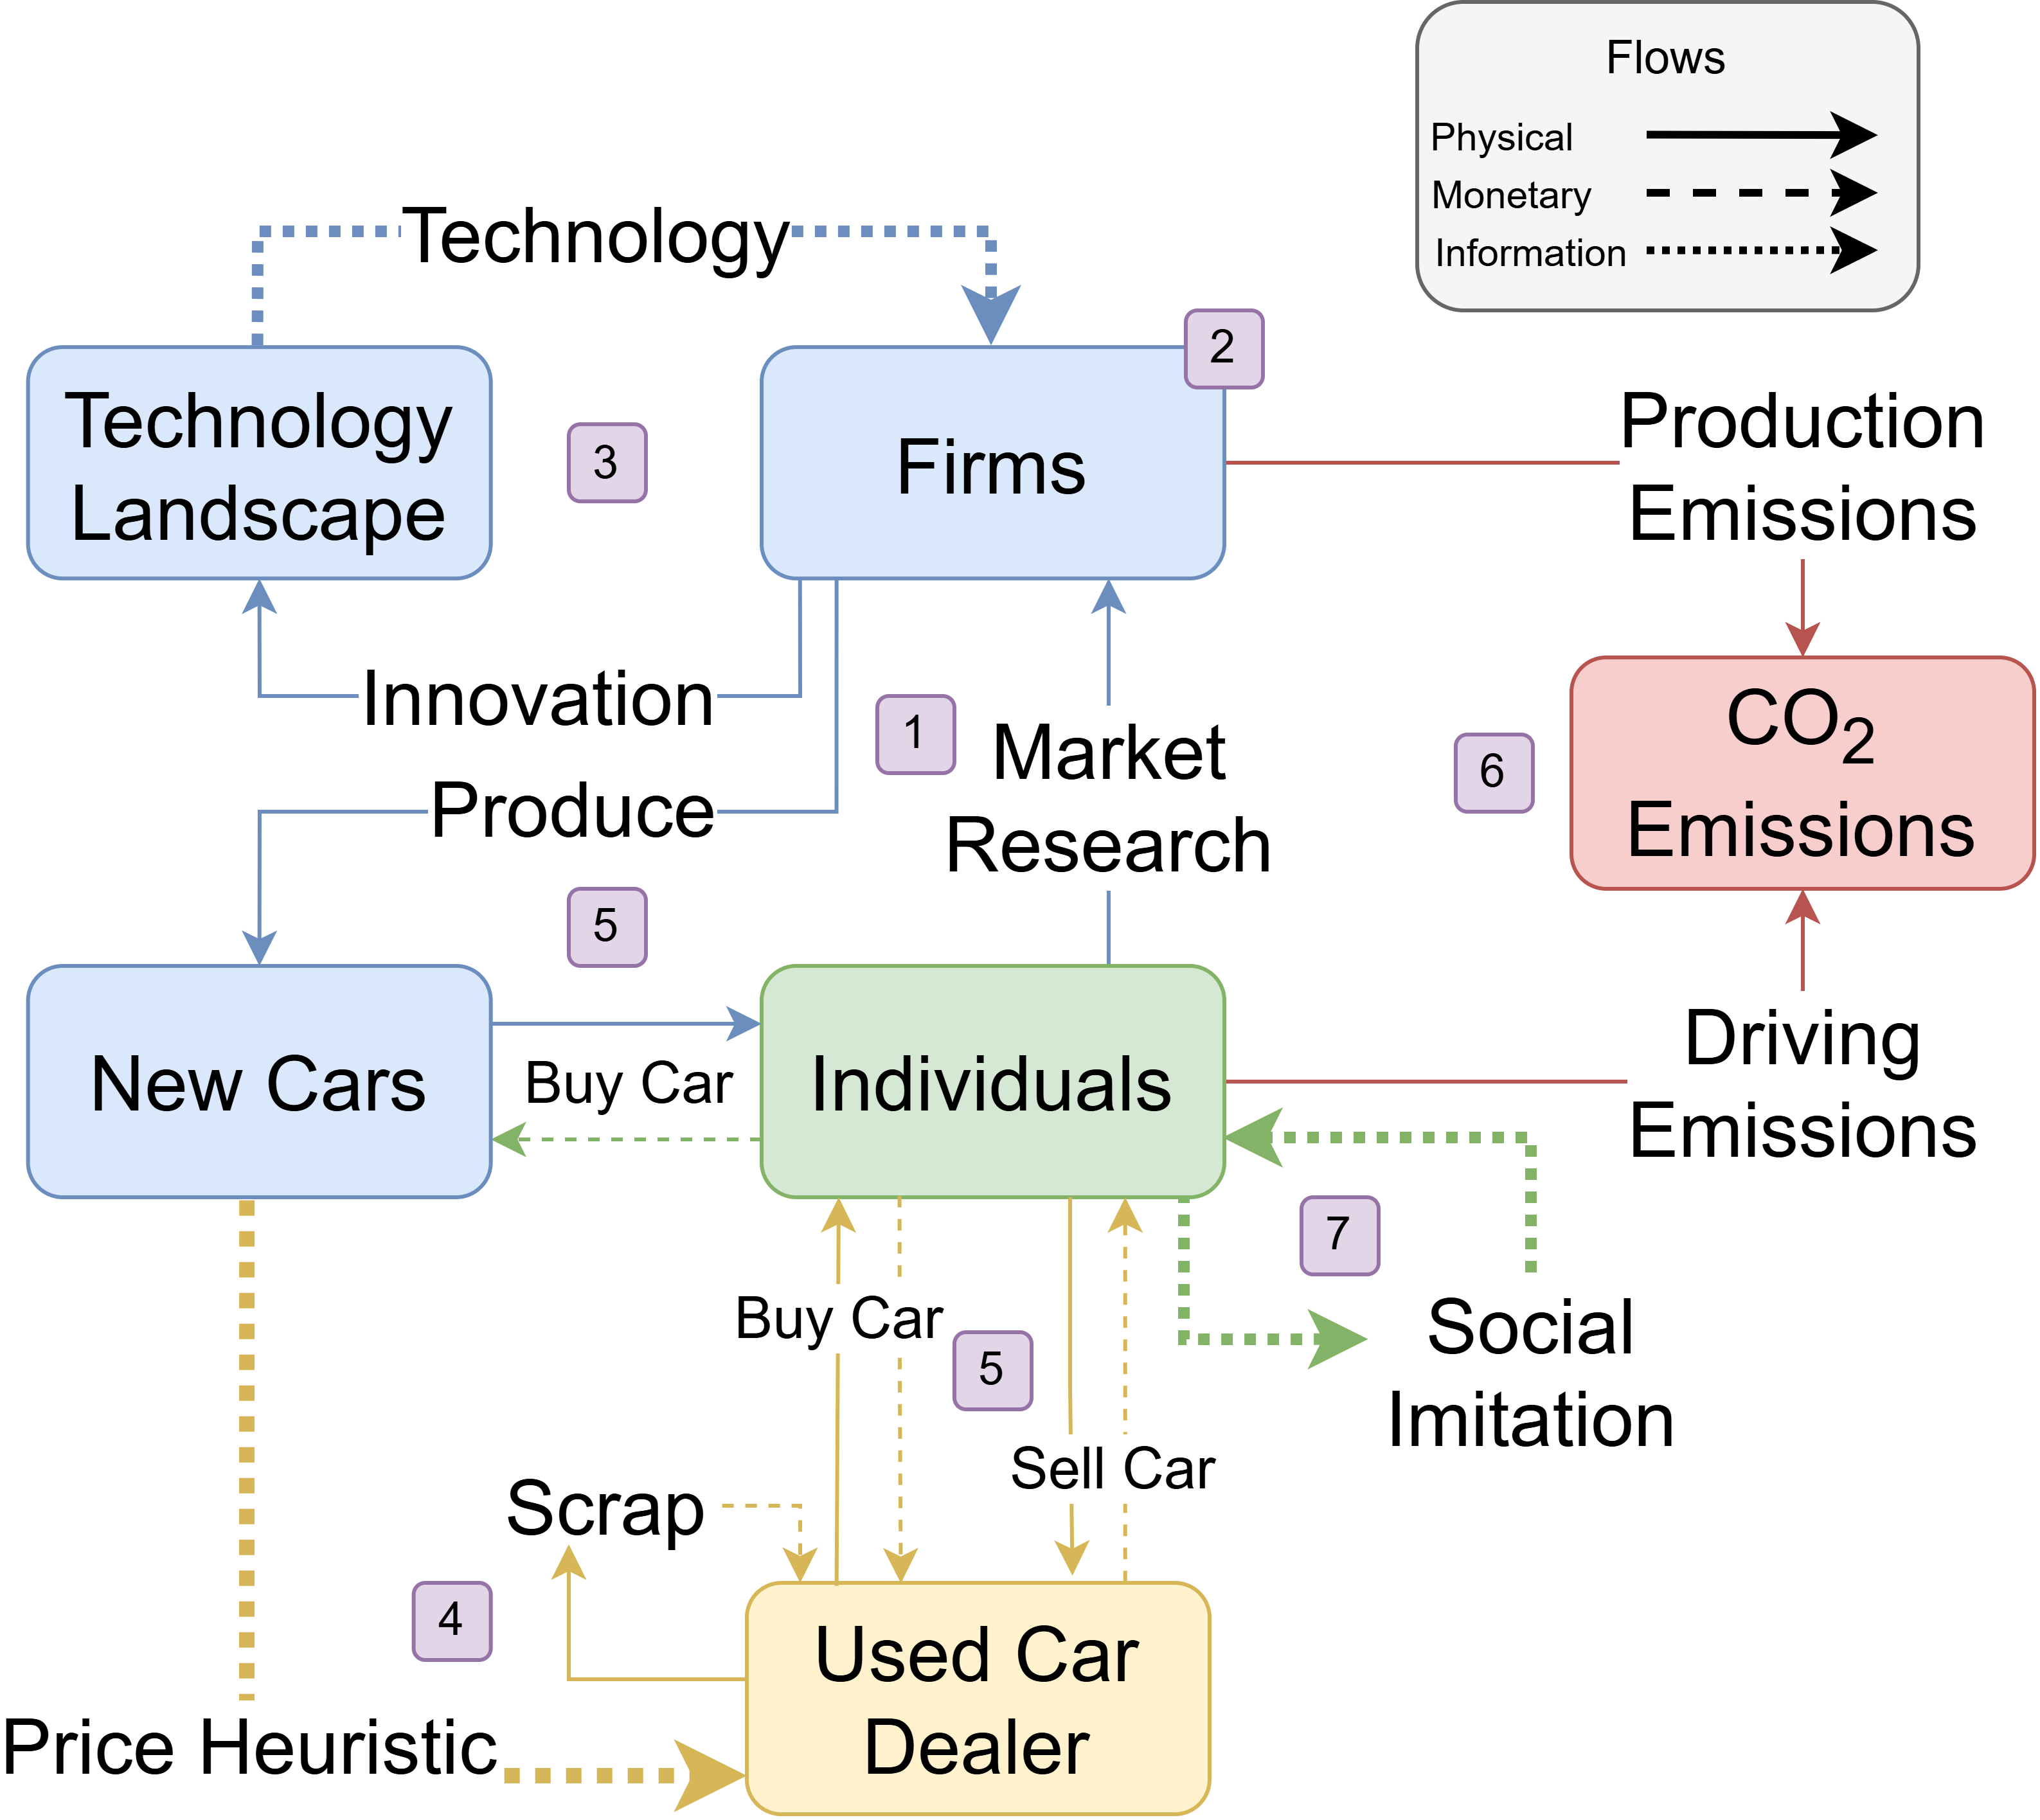
\includegraphics[width=0.75\linewidth]{Figure_1.png}
		\caption{Model structure. Numbered labels indicate sequence in model update (exogenous variables update not included).}
		\label{fig:diagram}
	\end{figure}

    The following steps describe the model update sequence within a single one-month time step:
    
        \begin{enumerate}
            \setcounter{enumi}{-1} % Starts the numbering at 0
            \item Current month's exogenous variables, including gasoline prices, electricity 
            prices, grid carbon intensity, and policy instruments are updated.
            \item Firms receive updated information on user EV consideration and vehicle 
            purchase, and observe the product mix and prices of competitors from the previous period.
            \item Firms are activated stochastically to update product mix and prices.
            \item Firms are activated stochastically to innovate.
            \item Cars on the used market are updated through the scrapping of old vehicles and prices are recalculated.
            \item Car users select from updates vehicles: either keeping current, buying a new or buying a used car. In the latter two cases also selling their car.
            \item Production and driving emissions are calculated.
            \item Social parameters, such as EV acceptance, are updated in anticipation of 
            the next step.
        \end{enumerate}

	\subsection{Car users} \label{Model_Users}
	Car users drive a fixed and heterogeneous distance each month \citep{zhang2025effect}. They are activated upon stochastic sequential activation to replace their car for a new or used car available on the market. Following the social imitation model, the willingness to consider buying an EV is updated at the end of the period. The model assumes each driver only has one car, as the US car-to-driver ratio has remained stable at $1.15$ from 2012 to 2023 (\hyperlink{https://www.bts.gov/browse-statistical-products-and-data/state-transportation-statistics/state-highway-travel}{Bureau of Transportation Statistics}). %From 2001 to 2009, only 30\% of U.S. adults were monomodal car users \citep{buehler2013trends}. 

    The literature on the determinants of EV choice highlights four classes of influencing factors \citep{singh_review_2020,pandita2024electrifying}: demographic factors (individual-intrinsic), situational factors (car features), contextual factors (infrastructure and policy), and psychological factors (societal dynamics). Demographic factors are embedded in the parametrized preference heterogeneity in our population. The charging infrastructure, an element within situational factors, is a given in this model. This section of the model description addresses the remaining two determinants. First, car choice depends on the situational factors of the considered alternatives, including quality and costs \citep{neves_technological_2019,hulshof2020willingness,pandita2024electrifying} and emissions \citep{hidrue2011willingness, biresselioglu_electric_2018,chen_assessing_2019}. Second, social influence is a crucial psychological factor \citep{sovacool2017experts,peng2024identifying}. Other factors such as marketing or habit \citep{singh_review_2020} are out of the scope of this study.
	
	\subsubsection{Car choice} \label{Users_Choice}
    
    Car users compare the lifecycle utility of their own car with that of the available used and new cars the user is willing to consider. The utility of a car is given by the willingness to pay for its quality and range, each of them with diminishing returns, minus its lifecycle costs and emissions \citep[p.4]{ipcc2022transport} (see Equation \ref{EQ_Utility} in Appendix \ref{model_equations}).    

    The lifecycle costs are given by the sum of the purchase price, net of the sale of the user's current car, and the discounted sum of the expected cost per kilometre (see Equation \ref{EQ_Lifecycle_Cost} in Appendix \ref{model_equations}). The lifecycle emissions are given by the manufacturing emissions if the car is new and the discounted sum of the expected emissions per kilometre (see Equation \ref{EQ_Lifecycle_Emissions} in Appendix \ref{model_equations}). When estimating future costs and emissions related to driving, car users factor in the depreciation of fuel efficiency taking place at the end of each time-step at a fixed rate. Given the uncertainty in gasoline and electricity markets, car users assume the future prices and emissions of gasoline and electricity to be the same as in the present period, as supported in the literature \citep{Anderson2013}.
	
	Comparing the utility for each of the alternative car choices (including their own), car users select one using a logit model \citep{McFadden1974} where the probability of selecting a car is proportional to its assigned utility (see Equation \ref{EQ_Probability_Choose_Car} in Appendix \ref{model_equations}). %The logit model includes an intensity of choice $\kappa>0$ such that a value of $\kappa = \inf$ indicates car users are utility maximising, whilst on the other extreme, for $\kappa = 0$, they choose cars randomly with equal probability.
	
	\subsubsection{Social imitation} \label{Users_SocialImitation}
	
	To represent the influence of peers on the choice of car type, we build on the threshold models of EV adoption \citep{eppstein2011agent, mccoy2014consumer, wang2023exploring}. We consider a fixed social network in which car users observe the proportion of EV owned by their neighbours. They consider buying an EV in the next period only if such a ratio is greater than or equal to their innovativeness threshold. This threshold is heterogeneous amongst car users, with a low threshold representing "innovators" who are willing to adopt new technologies, whilst a high threshold corresponds to "laggards" who will only consider moving away from the established technology once it is very common in their network neighbourhood (see Equation \ref{EQ_ConsiderBuy} in Appendix \ref{model_equations}).
	
	The result of the threshold model is that car users may not adopt EVs even if they have high utility. This structure captures the gap between behaviour and attitudes or beliefs in which car users may have sufficient desire (high utility) to pursue pro-environmental behaviours but do not do so due to other limiting factors \citep{kollmuss2002mind}, such as the lack of an established social norm. Thus, it is possible for car users to have a high willingness to pay for reducing emissions while being responsible for high emissions due to driving an ICEV. On the other hand, with policy intervention, social imitation dynamics can amplify the policy effect by increasing the visibility of EVs \citep{konc2021social}.    
	
	Social interaction is structured using a small-world network \citep{watts1998collective} to replicate word-of-mouth social interactions in highly clustered social circles where neighbours are also likely to become friends. This network is formed by first arranging car users in a ring, with each person connected to a homogeneous number of nearest neighbours, a fixed number of connections each to their nearest neighbours. Then the symmetry of the network is broken up by introducing long-range weak ties across the network through probabilistic re-wiring of connections.
	
	\subsection{Car supply}
	Manufacturers sell multiple car designs that are produced on demand. Upon stochastic activation, they update the car types on sale and their respective prices in line with profit maximisation. For tractability, we assume that car manufacturers face constant marginal production costs and are not subject to binding capacity or financial constraints. We acknowledge that factors such as carbon lock-in \citep{unruh2000understanding,unruh2002escaping} and the availability of venture capital for risky innovation \citep{mazzucato2013financing,mazzucato2017public} can shape technological transitions. However, we argue that these constraints are unlikely to be binding in developed urbanisations with an established charging infrastructure. In such settings, the relevant manufacturers are multinational firms integrated into global supply chains, with access to capital markets and the ability to source physical inputs on global markets. As long as EV production remains profitable at prevailing prices, neither financial liquidity nor short-term production bottlenecks constitutes a structural barrier to the transition trajectories we simulate.
	
	Following the Segmentation, Targeting and Positioning framework \citep{kotler1989mass}, manufacturers supply car designs targeting a specific consumer segment. A consumer segment is defined as a relatively homogeneous group of customers with particular needs and preferences \citep{lynn2012segmenting}. Consumer segments are formed on the basis of EV acceptance, willingness to pay for quality and willingness to pay for emissions reduction, covering the most relevant determinants of car choice after controlling for socio-demographic attributes \citep{axsen2013vehicles,keyes2018vehicles,jang2021vehicles}. For example, the Tesla Model S might appeal to a segment characterised by rich individuals who have high willingness to pay for emissions and are willing to buy an EV. 
	
	\subsubsection{Technology choice and pricing}\label{Supply:Choice_Pricing}
	Manufacturers evaluate the expected profit at each consumer segment of each car type using known technologies. The expected profit is given by the marginal profit, the size of the segment population, and the expected market share within the segment (see Equation \ref{EQ_Estimated_Profit_Segment} in Appendix \ref{model_equations}). This expected in-segment market share depends on the attributes of the car and the state of competition in that segment (over the last 12 months) (see Equation \ref{EQ_Competition_Segment} in Appendix \ref{model_equations}). Such that a less competitive car within a given segment receives a lower expected market share and thus is less attractive for production by a firm. Crucially, it is also consistent with the discrete choice consumption model, where the price is defined to maximise expected profits (see Equation \ref{EQ_Optimal_Price_Segment} in Appendix \ref{model_equations}).
	
	The choice of car types being supplied is resolved heuristically. Manufacturers include in their supply line the most profitable car targeted at a specific segment. Once the segment is satisfied, the selected price is locked in. The remaining segments are satisfied by sequentially selecting the most profitable car. Note that already selected cars cannot change their price for a different, potentially poorer, segment, meaning that they may be less competitive relative to unselected cars (see subsection \ref{Supply:Choice_Pricing} in Appendix \ref{model_equations} for a full description). As a result, a car may be produced to satisfy multiple segments at a single price if it outperforms other designs. %   where the expected profits of unselected cars targeted at their most profitable remaining segment are compared to that of the selected cars with the profit-maximizing price for the selected segments 
	
	By assuming that all manufacturers target all segments, we abstract from brand-reputation considerations. This simplification allows us to focus on the interaction between innovation and adoption, especially in the context of transition policies in the car industry. However, to encourage specialisation into specific segments, we limit the number of cars that may be produced by a single manufacturer to the total number of segments and limit the number of technologies a manufacturer can retain in its memory. This assumption follows from the strategic consideration that firms avoid cannibalising their earnings by supplying new products.  
	
	\subsubsection{Innovation} \label{Supply:Innovation}
	Car manufacturers innovate and learn technology to produce a new car type with unique characteristics. We use NK models to conceptualise innovation \citep{levinthal1997adaptation,rivkin_2000,baumann_siggelkow_2013}. In this framework, technologies are distributed on a map where local movements lead to changes in product attributes. NK models enable the representation of complex technological landscapes with multiple local solutions, accounting for the path-dependent nature of innovation. This assumption allows the capture of heterogeneous abilities to adopt technologies, or absorptive capacity \citep{cohen1990absorptive}, which are gained with path-dependent experience \citep{nelson1977search}.
	
	Manufacturers are engaged in a parallel search in the landscapes for ICEVs and EVs. These landscapes map for each combination of inputs the vector of attributes that define a technology. These attributes are quality, unit production cost, and fuel efficiency. Additionally, we add the battery size as an extra dimension in the EV landscape, accounting for potential innovations in the battery sector \citep{yao2025critically}. Thus, firms cannot easily produce EVs with high battery capacity for a low-cost consumer market due to additional innovation complexity.
    
    We limit innovation to the development of one single car, thus making the choice to develop ICEVs or EVs exclusive. We capture the probability of failed innovations by activating each firm's innovation submodule stochastically \citep{nelson1977search}. From an array of observed new car vintages, given by local improvements from past search (see Equation \ref{EQ_NeighborTechnologies} in Appendix \ref{model_equations}), firms observe the attributes of the alternative new vintages and strategically decide the next innovation based on profit expectations. Mirroring consumer car choice, firms use a logit model to choose which innovative design to pursue, with an intensity of choice parameter that determines the balance of exploration and exploitation \citep{Puranam2015} (see Equation \ref{EQ_SearchedTechnology} in Appendix \ref{model_equations}). A lower intensity of choice value means that firms will be more willing to consider alternative designs that currently may not be market leaders, but after additional innovation might.
	
	As in previous studies \citep{jain2014memory,bassart2026mixing}, manufacturers discard previously searched solutions when forming the set of candidate technologies to explore. This set contains all the unexplored neighbouring technologies with respect to the past search location on each landscape. We include the past search location, allowing the possibility of not searching if there are no attractive alternatives. Once a new design has been researched and the memory capacity is exceeded, the oldest car design not in production is forgotten. The limited memory capacity is a cognitive limitation whereby the searching agent economises cognitive power by forgetting unused solutions (see Equation \ref{EQ_MemoryUpdate} in Appendix \ref{model_equations}).  %Memory constraints are used in search algorithms inspired by animal behaviour as a form of escaping local solutions \citep{Tang_2012}. 
	
	\subsubsection{Used cars} \label{Model:Used_Cars}
    The used car market represents the majority of car purchases in the US\footnote{\href{https://www.statista.com/statistics/183713/value-of-us-passenger-cas-sales-and-leases-since-1990/}{Statista}}, providing an affordable alternative for low-income users. This model chooses a parsimonious approach for the representation of the market for used cars, where dealers are consolidated into a single entity that sets the purchase and sale prices of used cars.
	
	The sale price of a used car is a fraction of the price of its most similar car on the market for new cars (see Equation \ref{EQ:Reference_Price} in Appendix \ref{model_equations}). The fraction is inversely proportional to the used car age, where the price depreciation rate of EVs is larger than that of ICEVs \citep{SCHLOTER20222Depreciation} (see Equation \ref{EQ:Sale_Price_Used} in Appendix \ref{model_equations}). The used car purchase price is a fraction of its sale price, given by a fixed target mark-up that serves as a proxy for the degree of monopsony in the market for used cars (see Equation \ref{EQ_Purchase_Price_Used} in Appendix \ref{model_equations}). Sale and purchase prices have an exogenous lower bound representing the car's scrap value. Cars with prices lower than their scrap value are removed from circulation (see Equation \ref{EQ_Active_Cars} in Appendix \ref{model_equations}). 
	
	\section{Data and calibration} \label{Sec_Cal_Val}
	We set the parameters of the model to the data for the state of California 2001 to 2023, where each simulated time step represents a month. Table \ref{model_parameters} contains a summary of the model parameters and their sources (for a full documentation, see Section 1 of the Supplementary Material), with the monetary units expressed in 2020 US dollars. 
    
    When available, we retrieve from official or survey data. This is the case for the price and emissions per kilowatt hour of gasoline and electricity, and the distribution of monthly distance driven. We extrapolate secondary data from previous studies to calibrate the willingness to pay for range increases and emissions reductions, the car attribute boundaries in the NK landscape (except for the abstract quality), the car scrap value, the discount rate, and the price depreciation rate of used cars.

    We set non-observable parameters at values within a reasonable order of magnitude, testing the relevance of a selection of them in a Sobol global sensitivity analysis (see Section 2 in the Supplementary Material). This applies to the parameter governing technological complexity, the research intensity of choice, the mark-up applied in the used car market, and the diminishing returns to utility with respect to quality. 
    
	We follow past history-friendly models \citep{MALERBA2008355,herrmann2017optimal} in limiting calibration to a small selection of key non-observable parameters: the consumer intensity of choice, the fuel efficiency depreciation rate, the distribution of consumer willingness to pay for quality, and the distribution of the innovativeness threshold. These parameters are indirectly calibrated to replicate the trend of EV uptake and percentage of EV sales in California (see \href{https://www.energy.ca.gov/files/zev-and-infrastructure-stats-data}{California Energy Commission} data). Additionally, our indirect calibration keeps output variables such as prices, market concentration or average car age within the observed ranges described in Table \ref{tab:replicate}.
	
	\begin{table}[!ht]
		\caption{Target variable ranges}
		\centering
		\label{tab:replicate}
		\begin{tabularx}{\textwidth}{c c X}
			\hline
			\textbf{Variable} & \textbf{Range} & \textbf{Source} \\
			\hline
			Price for new cars & 25th \%: $\$32,359.41$, 75th \%:\$$57,784.66$ & \citep[Figure II]{Grieco2024MarketPower} \\
			Herfindahl-Hirshman index & ($.11$-$.18$) & \citep[Figure II]{Grieco2024MarketPower} \\
			Average car age between & ($10$-$12$) years & \href{https://www.bts.gov/content/average-age-automobiles-and-trucks-operation-united-states}{Bureau of Transportation Statistics} \\
			\hline
		\end{tabularx}
	\end{table}
	
	Since the willingness to pay for the quality parameter mostly affects the price level, we determine its median value analytically in such a way that the optimal price of an ICEV with average features targeted at a consumer with average willingness to pay equals the observed average price. Then, we distribute this value according to the Californian income distribution, assigning a higher willingness to pay to richer agents.  
	
	For the users' intensity of choice and the depreciation rate of car efficiency, we perform a grid search to match the stylised facts of car price range and age, iteratively narrowing the search space until matching the trends for EV uptake while keeping the other target variables within their observed ranges. Lastly, a beta distribution is used to define the heterogeneous values of car users' EV consideration thresholds.
    
    Given the high computation cost, we use simulation-based Bayesian inference \citep{papamakarios2016fast,cranmer2020frontier, dyer2024black} to calibrate the beta distribution values to match EV uptake between 2010-23 (see Figure \ref{fig:preferences} in Appendix \ref{Appendix:Additional_Figures}, for a representative distribution of the willingness-to-pay parameters, distances and innovativeness values). %Implementing a multi-round Neural Posterior Estimation (NPE) from the $\textit{sbi}$ \citep{tejero-cantero2020sbi} Python package, the EV adoption output from many model runs is used to train a mixture density network to approximate the posterior distribution over the beta parameters that determine the threshold distribution.
	
	We simulate a population of $3,000$ car users and $16$ car manufacturers \citep{Grieco2024MarketPower}. The model simulates a burn-in period of 15 years (180 time-steps) before the calibration period. The model is initialised with car manufacturers being placed at one Hamming distance from the worst technology when evaluated at the median segment, and car users owning a random car among those manufacturers can produce. During the burn-in period, manufacturers improve and sell ICEVs, while EV search and production are not permitted until the calibration period starts.   
	
	In order to account for existing EV support policies, we feature a simplified version of the federal and state rebate assigned to EVs \citep{CARB1990LEV, CARB1990hearing,CARB1990proposed} from 2010-23, discounting a flat amount of $\$10,000$ to new EVs and $\$1,000$ to used EVs. In addition, the implemented carbon taxes are already included in the imported prices for gasoline and electricity. We do not model the existing fuel efficiency standards or the EV sale mandates stipulated in the ZEV Californian plan, as regulatory measures are out of the scope of the present research and, consequently, the model does not capture side effects of regulation such as firm relocation, political influence, and compliance flexibility \citep{Wesseling2014Political,wesseling2015exploring}.   
	
	Figure \ref{fig:validation_plots} shows the model projections for the EV uptake and percentage of EV sales (top left), prices of new and used EVs and ICEVs (top right), market concentration (bottom right), and average car age (bottom left). The simulated values are the average over $64$ Monte Carlo simulations. These plots validate our indirect calibration exercise, given that the projections of EV uptake and sales closely match the real data and that prices, market concentration, and average car age are mostly within the ranges described in Table \ref{tab:replicate}. 
	
	\begin{figure}[!ht]
		\centering
		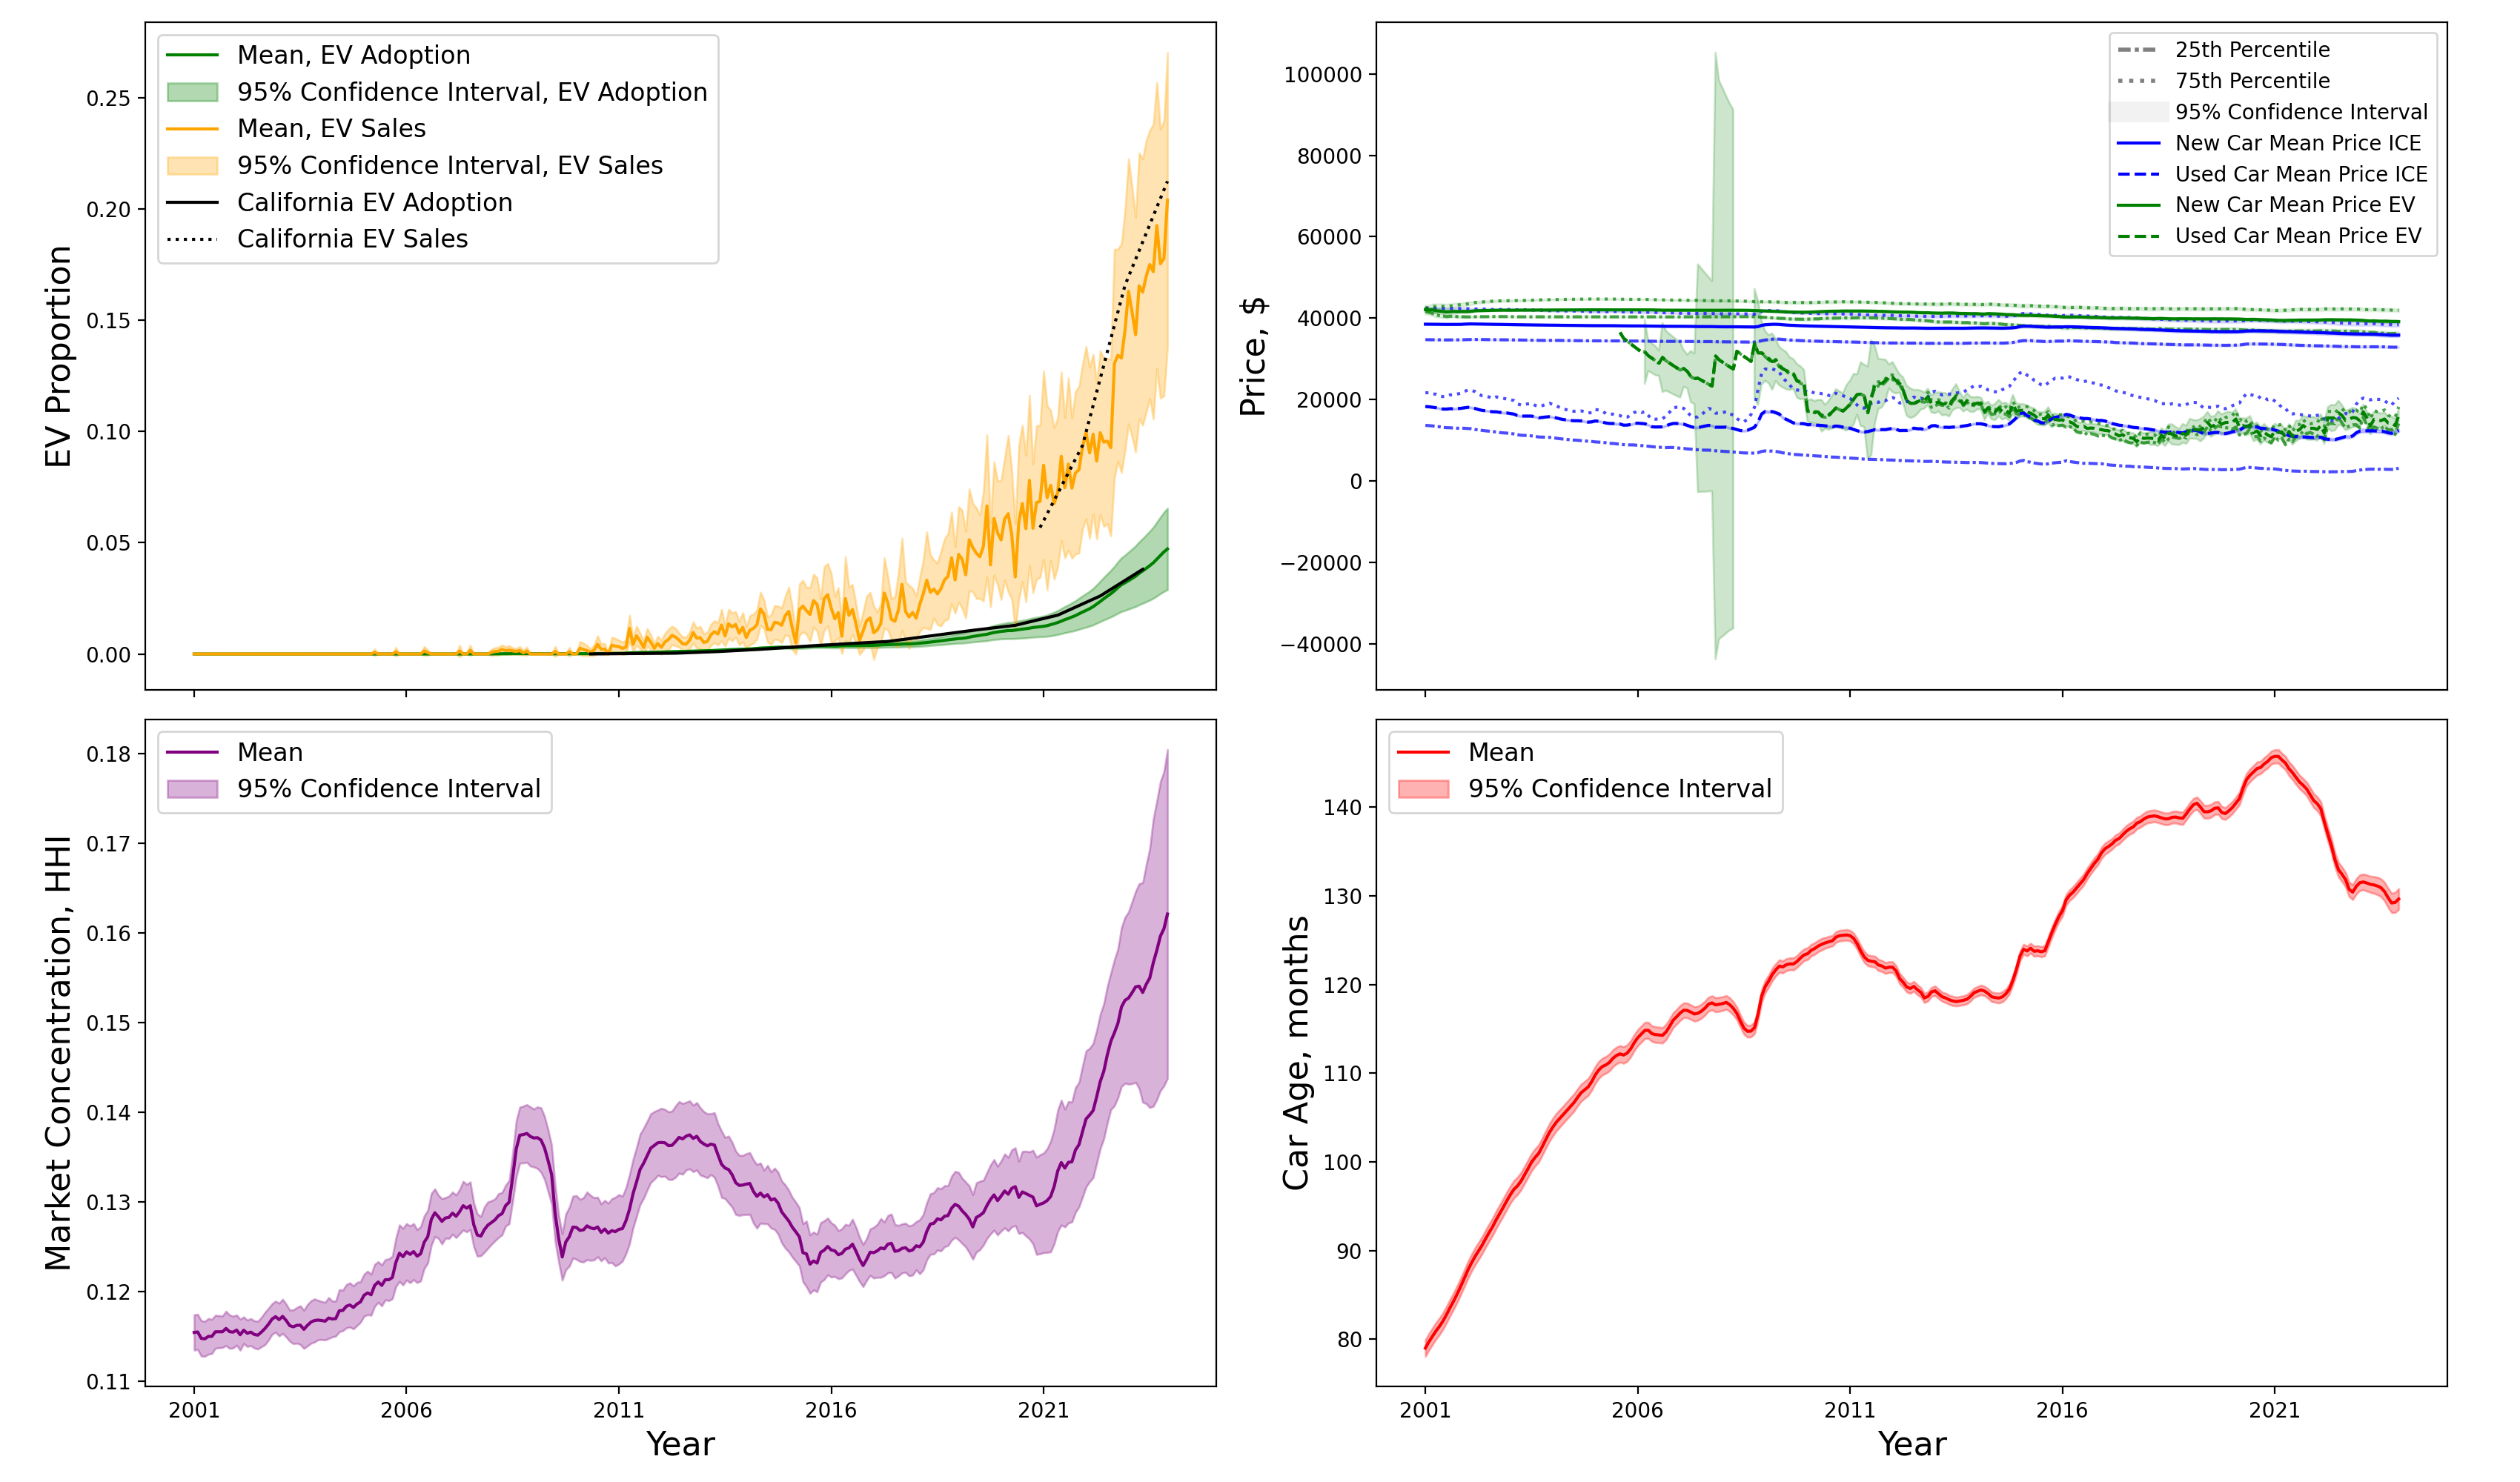
\includegraphics[width=0.9\linewidth]{Figure_2.png}
		\caption{Simulation of key model outputs from 2001 to 2023. EV uptake and EV sales, in percent (top left); Retail prices for new and used ICEVs and EVs, in dollars (top right); Herfindahl-Hirschman Index, in percent (bottom left); and, average car age, in months (bottom right).}
		\label{fig:validation_plots}
	\end{figure}

    To assess the role of the used car market on EV uptake during the calibration and policy period we varying the total market size, see Appendix Figure \ref{fig:used_car}. In the case where the used-car market is disregarded, EV uptake is much higher as those price-sensitive individuals who would previously have bought cheap ICEVs no longer have the option. Instead, these individuals purchase EVs that are competitive through their low-per kilometre cost. This result highlights the importance of including used car markets in models of transport decarbonisation to avoid overestimating future EV adoption. However, up to a certain capacity, adding more used car capacity has little additional impact on EV uptake. Thus, we argue that by setting fleet size to \textcolor{red}{10} \textcolor{yellow}{50}\% of population, we capture key dynamics and reduce computational cost per simulation. Nonetheless, the market size remains an order of magnitude larger than the number of used cars sold per time step, ensuring ample selection choices. 
	
	\section{Policy experiments} \label{Sec_res} 
	\subsection{Experimental setup}\label{Res_Setup}
	In this study, we focus exclusively on market-based policies. While other policy instruments, such as regulations, standards, information provision, or additional charging infrastructure, are relevant \citep{guven2026assessing,Juntunen2026}, our analysis is focused on market-based policies due to their compatibility with long-run incentives \citep{Gebhardt2026} and easy calculation of net costs. 
	
	Policies are treated as exogenous, and car manufacturers and users immediately incorporate the price signals into their behaviour when making choices. However, we disregard the role of expectations regarding policy stringency \citep{helm2003credible,aghion2019path}, with agents assuming that policies will be permanent. Note that the rebate on new and used cars implemented during the calibration period is removed to avoid interference with other policies. Policies are applied from January 2024 at the their full intensity and are then constant over the policy period (2024-35).
	
	We consider the interventions listed below:
	
	\begin{itemize}
		\item \textbf{Carbon price}: The gasoline and electricity cost per kilowatt hour increases by $\$\tau_1$ for each kilogram of $CO_2$. This policy aims to increase the attractiveness of EVs relative to ICEVs based on their lower emissions per kilometre while increasing the public budget \citep{Hardman2019Understanding}.
		\item \textbf{Subsidy on EV charging electricity}: The electricity cost per kilowatt hour is subsidized by $\tau_2\%$. This policy aims to increase the attractiveness of EVs by decreasing the cost per kilometre. This subsidy can be envisioned as applying to public or private EV charging stations \citep{Kwon2018Evaluation}. 
		\item \textbf{Rebate for new EVs}: The purchase price of new EVs decreases by $\$\tau_3$, with a zero-lower bound. This policy aims to increase EV adoption by reducing its sale cost while increasing producers' profits who incorporate the subsidy into their price-setting function \citep{Lodhia2024Assessment}. 
		\item \textbf{Rebate for used EVs}: The purchase price of used EVs decreases by $\$\tau_4$, with a zero-lower bound. This policy aims to increase EV sales among more price-sensitive car users, and as a consequence, reduce total $CO_2$ emissions by minimising the production of new cars \citep{Lodhia2024Assessment}. 
		\item \textbf{Production subsidy}: The production cost for manufacturing EVs decreases by $\$\tau_5$, with a zero-lower bound. Like the new car rebate, this policy is expected to increase EV adoption and producers' profits, thus motivating EV innovation. However, this policy is expected to induce a lower reduction in prices due to rent seeking \citep{OECD2025Subsidies}.
	\end{itemize}

    Note that the zero-lower bound, found in the rebate for new EVs, the rebate for used EVs and the production subsidy, applies to the final purchase price of the vehicle after applying the subsidy. This prevents the price of cars from becoming negative.

	The policy experiments are evaluated for the period 2024-2035 ($144$ time steps), according to the ZEV mandate timeline. In accordance with the Californian ZEV Plan, we assume a linear decarbonisation of the electricity grid, such that by the end of the policy period, emissions per kilowatt-hour of electricity are reduced by 90\% by 2035. The prices for electricity and gasoline before the policy implementation are fixed at the last observed data point \citep{Anderson2013}. To assess the sensitivity of the BAU scenario in the Supplementary Material Section 2.4 we consider differing degrees of grid decarbonisation and changes in electricity prices.
    
    First, we individually simulate each policy instrument using grid search to vary the policy stringency. The grid search simulates $100$ policy values for each instrument, ranging from $0$ to the maximum values shown in Table \ref{Tab:Policy_Intensity}. The maximum values were chosen to represent an extreme value in order to test the limits of each individual policy.   
	\begin{table}[h]
		\centering
		\caption{Maximum policy intensity evaluated in the single-instrument scenario.}
		\begin{tabular}{cc}  \hline
			\textbf{Instrument} &  \textbf{Maximum intensity} \\
			\hline
			Carbon price &  $1500\$/TCO_2$ \\
			Subsidy on electricity & $100\%$ \\
			New car rebates & $\$50,000$ \\
			Used car rebates & $\$50,000$ \\
			Manufacturing cost subsidy & $\$50,000$ \\
			\hline
		\end{tabular}
		\label{Tab:Policy_Intensity}
	\end{table}
	
	Having evaluated the effect of the policy stringency on multiple measures, we calculate the intensity of the policy required to achieve a target 95\% EV uptake on average across simulations, allowing for a 1\% discrepancy. We employ a Bayesian optimisation model \citep{head_2021_5565057} using a Gaussian process to build a surrogate model that predicts how EV uptake responds to the intensity of the policy. The uncertainty about expected EV uptake decreases with the number of simulation runs, where the selected policy intensity value is chosen by maximising the expected improvement acquisition function. In doing so, exploration and exploitation are balanced by prioritising large uncertainty and a better fit simultaneously.
	
	The values obtained are used as boundaries to find policy mixes that achieve the target uptake. For each pair of policies, the intensity of one instrument is fixed at $10$ equally distributed partitions of the optimal intensity. Using the same Bayesian optimisation method, we evaluated the intensity of the policy required by the pairing policy to achieve the target uptake. This analysis excludes pairs that do not include policies that can trigger a transition when implemented in isolation.
	
	Finally, we show the transition path of each policy pair. The intensity chosen for each combination is set to minimise the maximum intensity of the two, relative to its maximal value detailed in Table \ref{Tab:Policy_Intensity}. This approach is followed by the consideration that large policy instrument intensities can be politically unfeasible or cause limit dynamics in the real world that our model cannot address. Furthermore, some combination of policies can produce positive synergistic effects \citep{van2021designing} that we aim to explore. In order to test the stability of the transition, we remove the policy instruments after December 2035 and continue the simulation until December 2050.
	
	\subsection{Policy results}
	\subsubsection{Individual policies}
	Figure \ref{fig:individual_policy_multiintensity1} shows the effect of each individual policy on EV uptake, net policy cost, \textcolor{green}{cumulative emissions}, cumulative utility, and profits.
	
	\begin{figure}[!ht]
		\centering
		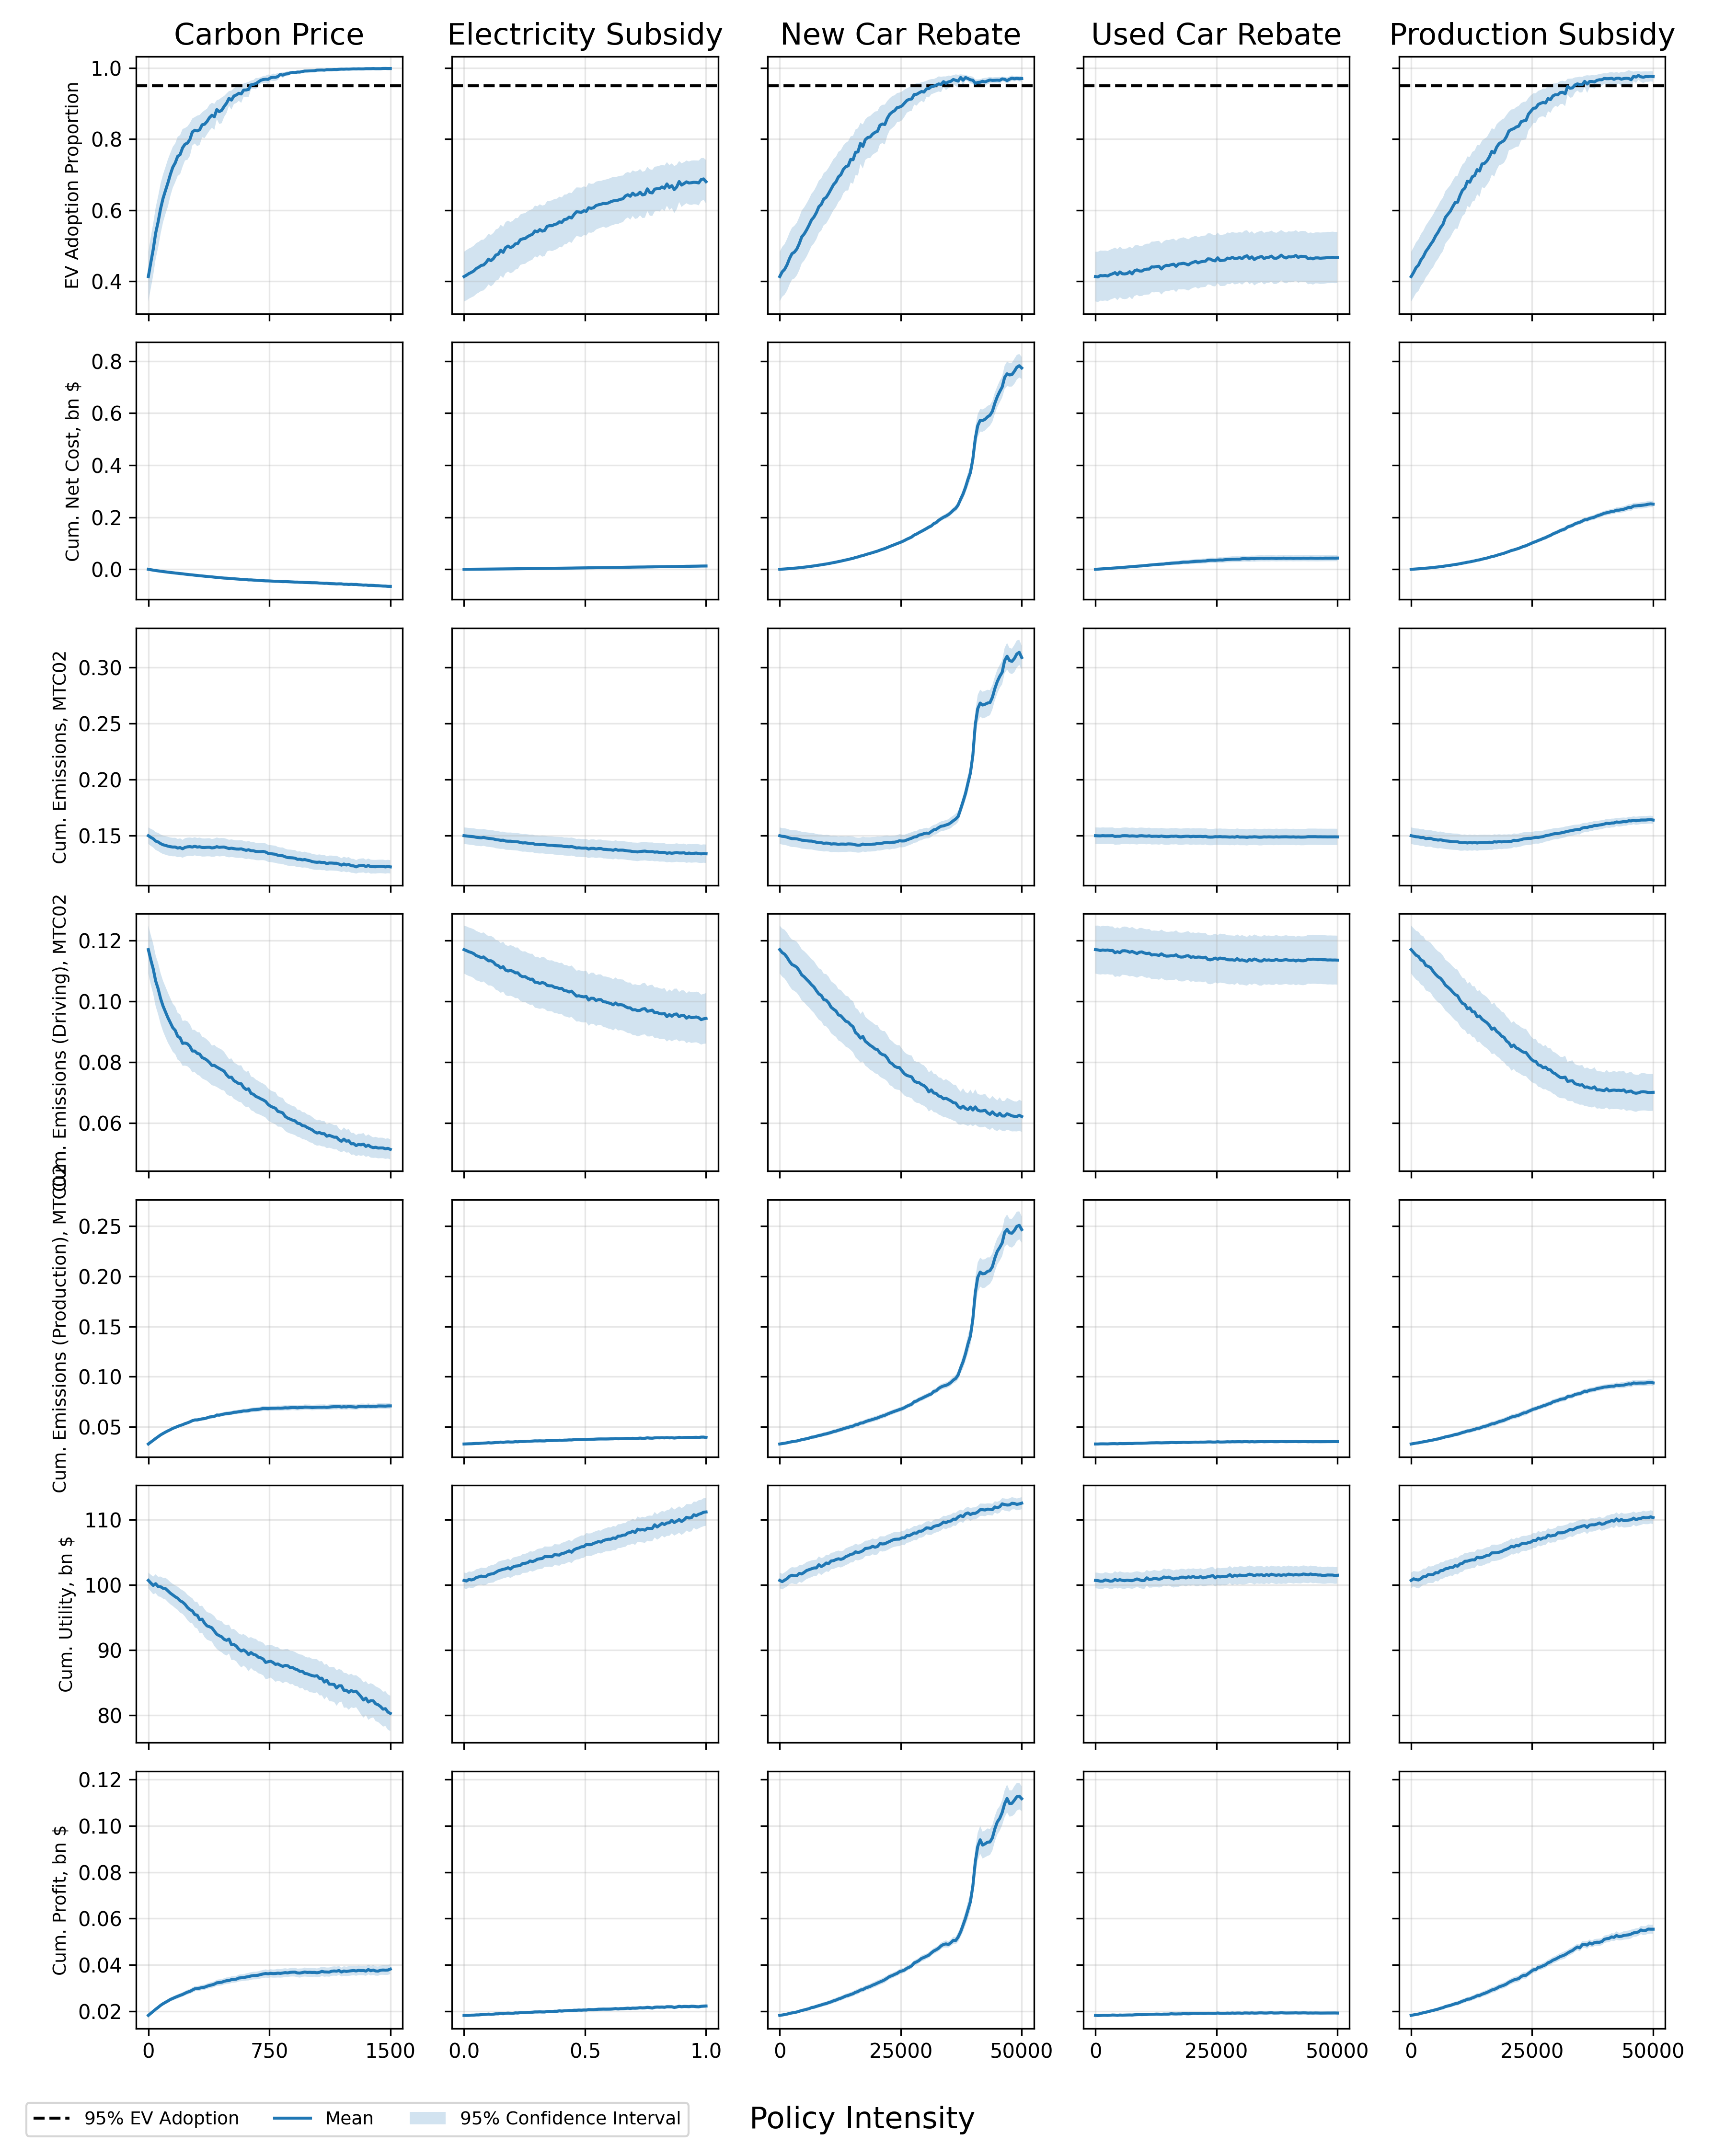
\includegraphics[width=0.8\linewidth]{Figure_3.png}
		\caption{Key model outputs for single policies.}
		\label{fig:individual_policy_multiintensity1}
	\end{figure}
	
	At low values of the carbon price, the proportion of EV adoption increases rapidly with a lower marginal increase from approximately \textcolor{yellow}{$\$200$} / T $CO_2$. Since the carbon price has unbounded effects with respect to intensity increases, it can achieve a complete transition at its extreme value, unlike the other policies. Government revenue increases with the carbon price, but with diminishing returns as a result of higher EV uptake. The manufacturing of new EVs is necessary to reach higher uptake and responds positively to the stringency of the carbon price, yet with diminishing returns. The diminishing effect of the carbon price is due to the heterogeneity among users, where those with low price and carbon sensitivity require a higher tax to change their behaviour. The production of new EVs increases manufacturers' profits and manufacturing carbon emissions, both cumulative over the period \textcolor{yellow}{2025}-2035. \textcolor{red}{The increase in manufacturing emissions compensates for the reductions in gasoline use, leading to higher total cumulative emissions in the medium-term. However, as shown in Section \ref{transition_stabilty}, this transitional spike reverses in the long run once the fleet has turned over.} \textcolor{green}{The reductions in gasoline use compensates for the increase in manufacturing emissions, leading to lower total cumulative emissions in the medium-term.} \textcolor{red}{Furthermore} \textcolor{green}{However}, consumer utility, cumulative over the \textcolor{yellow}{2025}-2035 period, decreases linearly with respect to the value of the carbon price. This is due to the strong negative effects of higher gasoline prices on non-EV-adopters. As a result, despite being the most effective instrument, the carbon price faces \textcolor{green}{a} severe political feasibility risk\textcolor{red}{s}, as reported in the literature \citep{maestre-andres_perceived_2019,savin2024carbon,mayol_analysis_2025}. \textcolor{green}{Finally, manufacturers' profits increase proportionally with EV adoption, which stems from an early replacement of the car fleet.}
	
	The electricity subsidy does not achieve 95\% EV uptake for any value. However, EV uptake increases linearly with the electricity subsidy, achieving an uptake of \textcolor{red}{60}\textcolor{green}{75}\% with free charging electricity. The budgetary impact of the policy is less than that of other policies due to the high fuel efficiency of EVs and the smaller policy impact on uptake. \textcolor{red}{Given that the policy is insufficient to trigger a substantial production of new EVs, cumulative $CO_2$ emissions decrease with the size of the subsidy. In this case, the larger manufacturing emissions do not offset the $CO_2$ savings from lower gasoline use.} \textcolor{green}{Cumulative emissions decrease with the subsidy intensity as a result of the higher adoption rates that result in a reduction of driving emissions.} Furthermore, both cumulative utility and profits linearly increase with the subsidy, the former being more reactive than the latter. 
	
	In the case of both the carbon price and the electricity subsidy, the policies affect all car users at all time steps, increasing the impact on utility relative to at-sale policies such as rebates or production subsidies. However, this is counteracted by the high annual discount rate used of 5\% \citep{busse2013consumers, greene2010consumers}, which limits the utility gains EVs have in their long-term behaviour caused by their high efficiency and lower operating costs. 
	
	The rebate for new cars \textcolor{red}{increases EV uptake linearly before reaching 95\% EV adoption} \textcolor{green}{achieves the 95\% adoption target at nearly its maximum level}. \textcolor{red}{However, high rebate values cause users to purchase new EVs more often as their price approaches zero. As a result, the total cumulative policy cost, the manufacturing emissions, and manufacturers' profits increase more than linearly with respect to the rebate size. In contrast, consumer utility increases linearly and reaches a maximum at the point where the rebate covers the full price of new EVs. These outcomes challenge the feasibility and usefulness of the policy.} \textcolor{green}{However, the policy costs increase more than linearly with respect to the subsidy size. As in the previous policies, the final cumulative emissions decrease with the subsidy size, with reductions in driving emissions compensating for increases in manufacturing emissions. Consumer utility and profits increase, with profits increasing exponentially with respect to the rebate size due to manufacturers' increased ability to capture rent.}
	
	In the case of the rebate for used cars, the lack of a pre-existing sizeable stock of used EVs makes the policy highly ineffective, having a negligible impact on any of the outcomes. 
	
	The production subsidy has similar effects to the rebate for new cars, since both policies directly affect the price of new EVs. However, its effects are milder as manufacturers are more able to capture rent. Due to higher retail prices, EV uptake does not reach 95\% for any production subsidy value. However, the policy-induced uptake at high subsidy values exceeds 90\%. The subsidies on manufacturing costs lead to lower turnover of EVs compared to the rebate for new cars, resulting in lower policy-induced increases in cumulative policy costs, $CO_2$ emissions \textcolor{green}{reductions}, users' utility, and manufacturers' profits.
	
	%Using Bayesian optimization methods, 
	We calculate the required policy stringency to achieve the uptake target of 95\% on average in different stochastic seed simulations. Table \ref{tab:policy_outcomes} shows the key outputs from the policy intensities compared to the business-as-usual (BAU) scenario.

    \textcolor{red}{
    \begin{table}[h!]
        \centering
        \caption{Outcomes of single policies at minimum intensity achieving a 95\% EV fleet}
        \label{tab:policy_outcomes}
        \begin{adjustbox}{width=\textwidth}
            \begin{tabular}{lccc}
                \toprule
                & \textbf{BAU} & \textbf{Carbon Price} & \textbf{New Car Rebate} \\
                \midrule
                \textbf{EV Adoption Proportion, ($\sigma$)} & 0.282 (0.247) & 0.951 (0.040) & 0.951 (0.064) \\
                \textbf{Intensity} & - & 674 $\$/TCO_2$ & $\$41479.30$ \\
                \textbf{Cumulative Net Cost, bn USD} & 0.000 & -0.038 & 0.160 \\
                \textbf{Cumulative Emissions, MT$CO_2$} & 144.74 & 126.40 & 123.78 \\
                \textbf{Cumulative Emissions (Driving), MT$CO_2$} & 117.26 & 62.67 & 63.48 \\
                \textbf{Cumulative Emissions (Production), MT$CO_2$} & 27.48 & 63.74 & 60.31 \\
                \textbf{Cumulative Profit, bn USD} & 0.020 & 0.044 & 0.040 \\
                \textbf{Cumulative Utility (2030), bn USD} & 4.997 & 3.735 & 5.331 \\
                \textbf{Cumulative Utility (2035), bn USD} & 10.009 & 8.985 & 11.024 \\
                \bottomrule
            \end{tabular}
        \end{adjustbox}
    \end{table}}

\textcolor{green}{
    \begin{table}[h!]
	\centering
	\caption{Outcomes of single policies at minimum intensity achieving a 95\% EV fleet}
	\label{tab:policy_outcomes}
	\begin{adjustbox}{width=\textwidth}
		\begin{tabular}{lccc}
			\toprule
			& \textbf{BAU} & \textbf{Carbon Price} & \textbf{New Car Rebate} \\
			\midrule
			\textbf{EV Adoption Proportion, ($\sigma$)} & 0.282 (0.247) & 0.951 (0.040) & 0.951 (0.064) \\
			\textbf{Intensity} & - & 674 $\$/TCO_2$ & $\$41479.30$ \\
			\textbf{Cumulative Net Cost, bn USD} & 0.000 & -0.038 & 0.160 \\
			\textbf{Cumulative Emissions, MT$CO_2$} & 144.74 & 126.40 & 123.78 \\
			\textbf{Cumulative Emissions (Driving), MT$CO_2$} & 117.26 & 62.67 & 63.48 \\
			\textbf{Cumulative Emissions (Production), MT$CO_2$} & 27.48 & 63.74 & 60.31 \\
			\textbf{Cumulative Profit, bn USD} & 0.020 & 0.044 & 0.040 \\
			\textbf{Cumulative Utility (2030), bn USD} & 4.997 & 3.735 & 5.331 \\
			\textbf{Cumulative Utility (2035), bn USD} & 10.009 & 8.985 & 11.024 \\
			\bottomrule
		\end{tabular}
	\end{adjustbox}
\end{table}}

	Our model demonstrates that a 95\% EV uptake by 2035 is possible with a carbon price near \textcolor{red}{$910\$/TCO_2$} \textcolor{green}{$674\$/TCO_2$} or with a rebate for new EVs near \textcolor{red}{$\$36875.57$} \textcolor{green}{\$41{,}479}. The suggested value for the carbon price is high relative to some estimates of the social cost of carbon (SCC) but not unheard of \citep{moore2024synthesis, bilal2024macroeconomic}. Likewise, that of the rebate for new cars is substantially larger than the currently implemented rebates worldwide, usually ranging between US\$2500 to US\$20,000 \cite{HARDMAN2017EVRebate}.

    \textcolor{green}{In terms of emissions reductions and cumulative manufacturing profits, both policies improve the BAU scenario with analogous magnitude. However,} beyond the difficulty of undergoing a highly stringent intervention, each of the policies face political feasibility challenges. Mainly, the carbon price induces lower cumulative consumer utility \textcolor{red}{with respect to the BAU scenario}, both in the short and in the medium run, while the rebate for new EVs leads to large policy costs. \textcolor{red}{Furthermore, both policies result in a net increase in cumulative emissions due to the transitional large-scale deployment of EVs. This effect is almost double with the EV rebate. However, the fact that the driving emissions in both cases are lower than in the BAU scenario indicates that the increase in overall emissions is transitional (see Section \ref{transition_stabilty}).}

    The single-policy simulations presented above yield required policy intensities that are extreme by any practical standard. We emphasise that these values should not be interpreted as policy prescriptions. Rather, they signal that, when accounting for the co-dependence of directed innovation and social imitation together with the used car market, relying on a single market-based instrument to overcome the coordination failure inherent in EV transitions is economically inefficient and politically unfeasible. This finding aligns with a broad consensus in the policy evaluation literature \citep{Bakker2013Policy,mccollum_interaction_2018,fan2025unfolding}. 
	
	\subsubsection{Policy pairs}
	As a consequence of the sizeable transitional costs and extreme policy intensity values, we now consider how policy mixes of two instruments may fare better in negating their individual weaknesses and reducing their values to more politically palpable levels. To this end, we compare the cumulative emissions resulting from each policy combination with their respective cumulative utility and net policy cost in the scatter plots shown in Figure \ref{fig:policy_pair}.
	
	\begin{figure}[!ht]
		\centering
		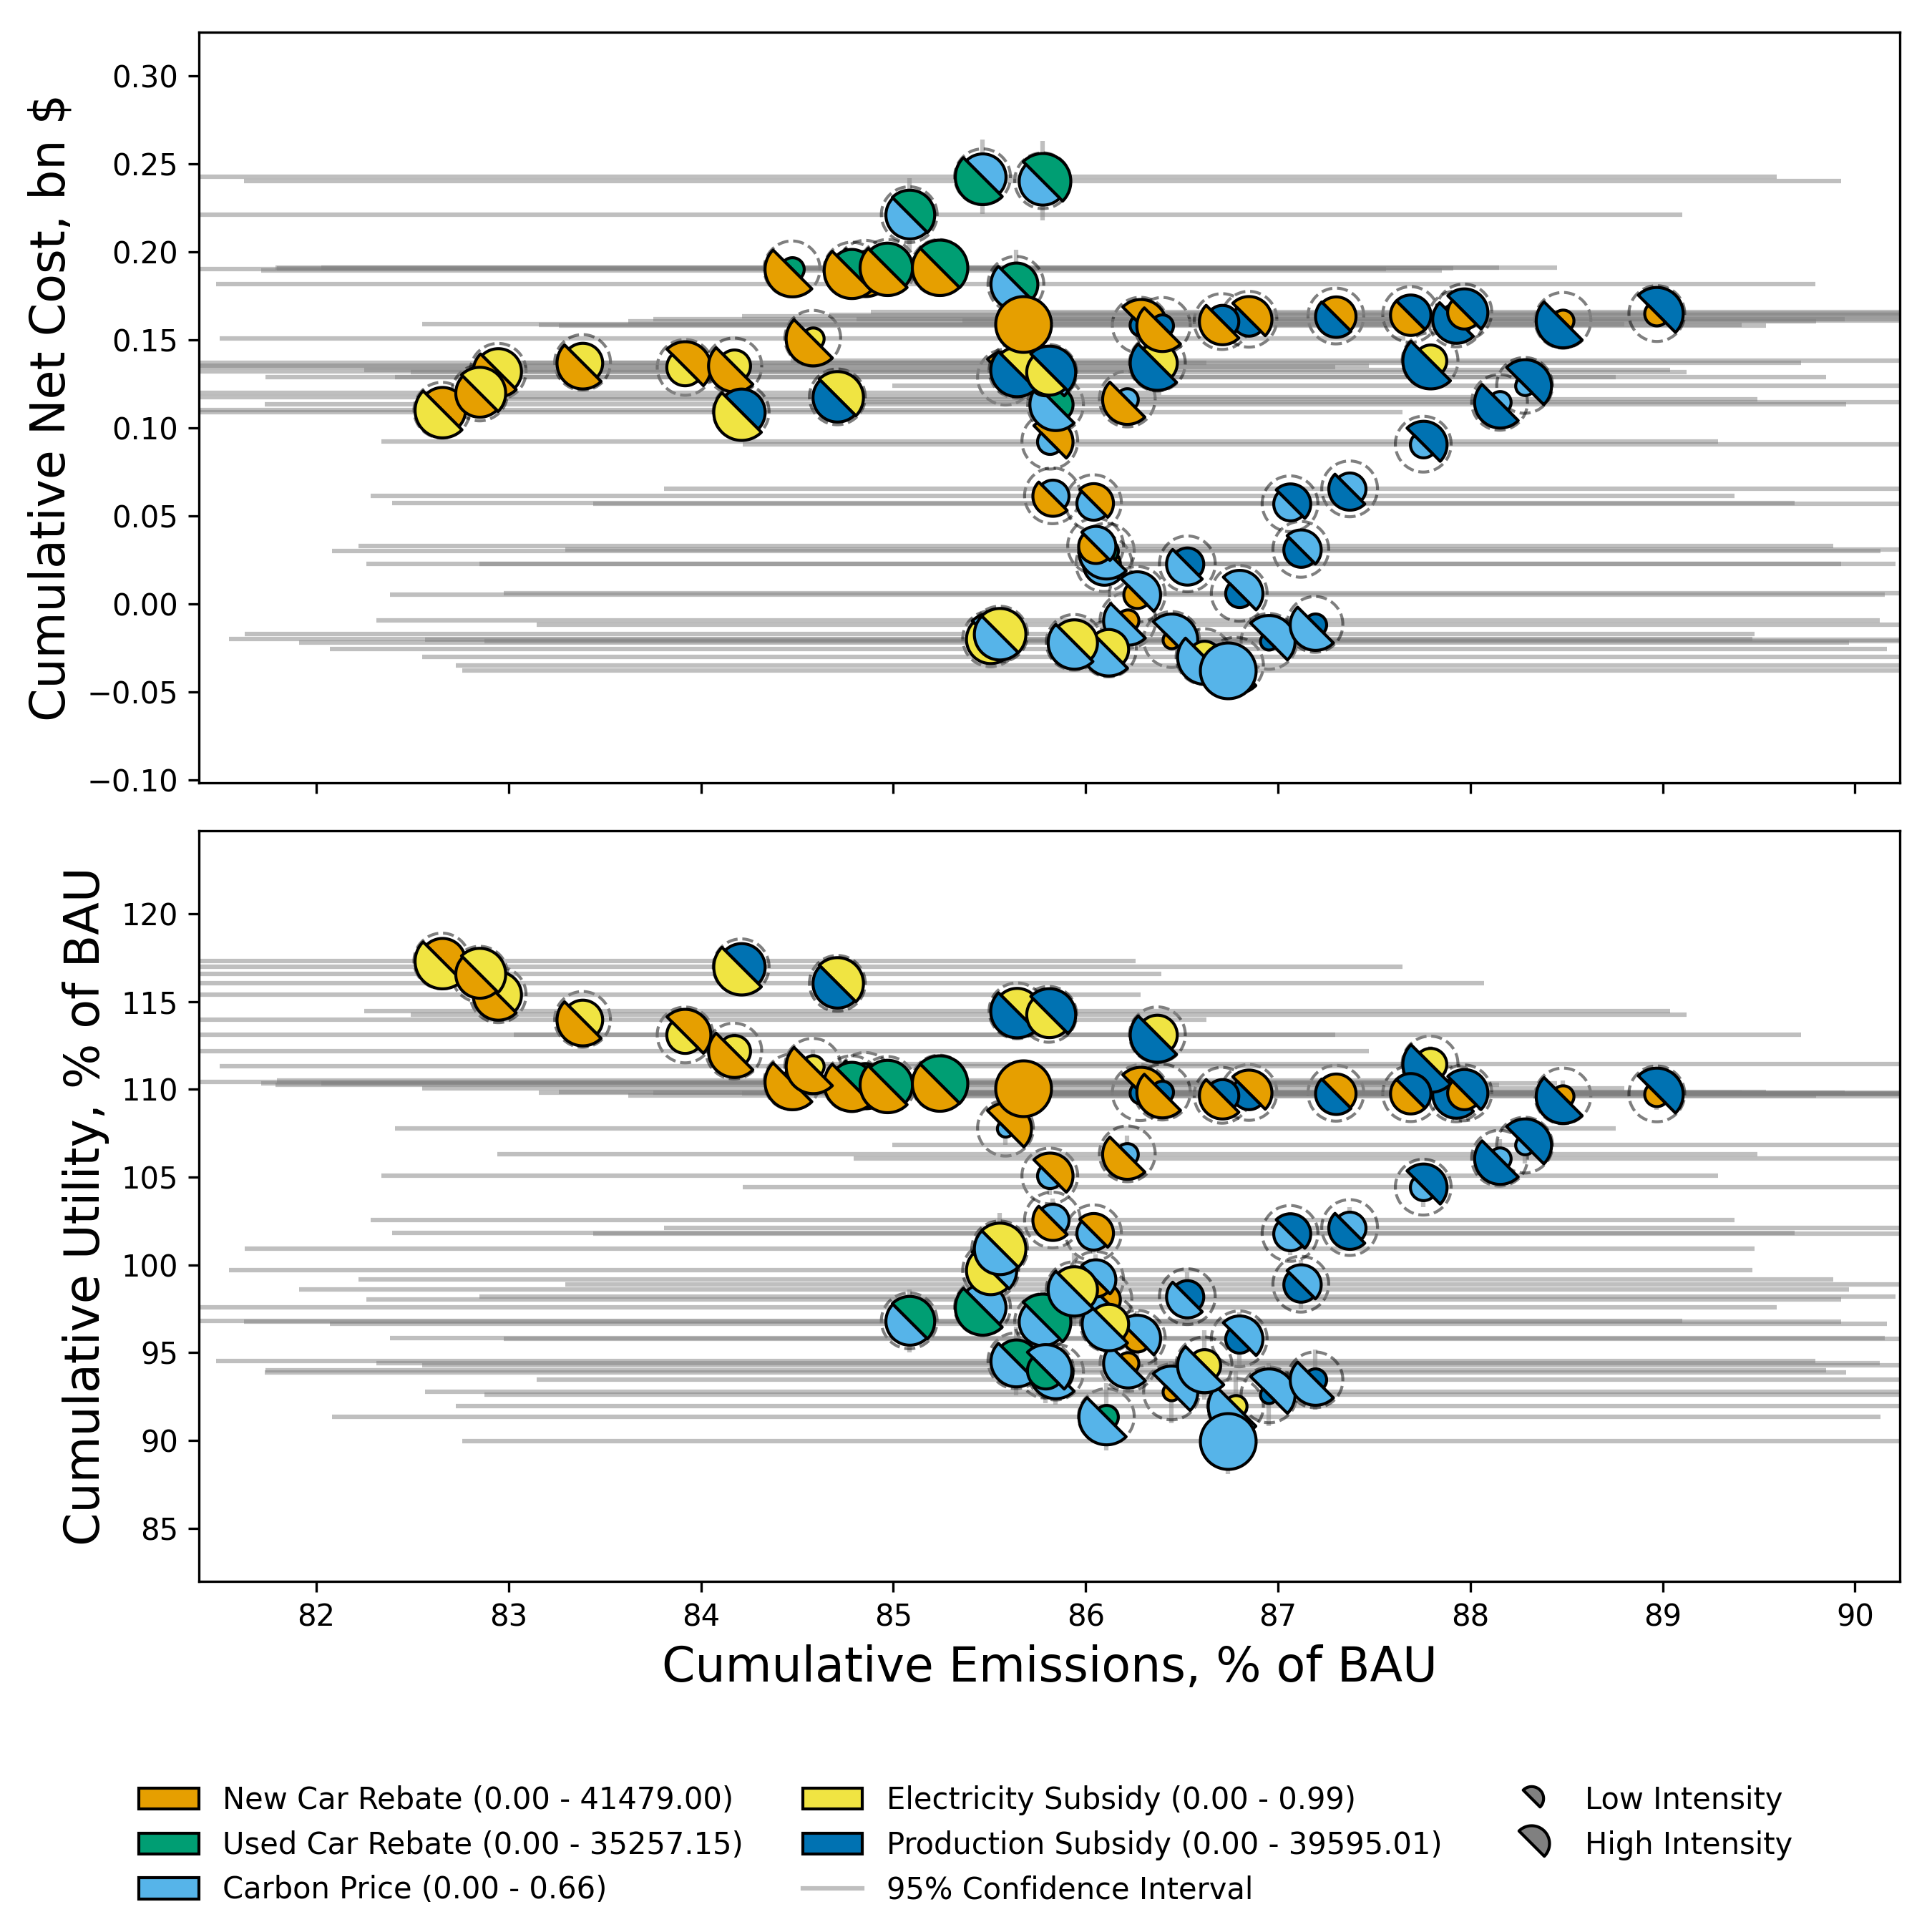
\includegraphics[width=0.75\linewidth]{Figure_4.png}
		\caption{Policy pairs outcomes that achieve 94-6\% EV adoption proportion, cumulative from \textcolor{yellow}{2024} to 2035. Policy intensity is indicated in half-circle size, where the full circle indicates the maximum intensity. Single instrument policies are shown as a full circle. BAU is shown in black as a reference.}
		\label{fig:policy_pair}
	\end{figure}  
	
	Figure \ref{fig:policy_pair} shows how instruments interact with one another in minimising the implied trade-offs exposed in Table \ref{tab:policy_outcomes}. Furthermore, it shows that policy combinations achieve substantial reductions in the policy intensity of both instruments, thereby improving the political acceptability of the transition. \textcolor{red}{This is particularly true with policy pairs involving a carbon price, a rebate for new EVs, or a production subsidy.} \textcolor{green}{Finally, all policies that lead to meet the 95\% adoption target result in a nearly 14\% reduction of cumulative emissions, with no statistically significant differences among the emission reduction levels of each policy.}
    
    Adding an electricity subsidy to the carbon price (yellow and \textcolor{red}{green} \textcolor{green}{light blue}) can substantially mitigate its costs in terms of utility\textcolor{green}{, improving that of the BAU scenario when the electricity subsidy is implemented at its maximum intensity}. The mechanism that allows this is two-fold. First, electricity subsidies reduce the lifecycle costs of EVs, compensating for the dissatisfaction of users who hold ICEVs. Second, electricity subsidies allow for reducing the carbon price to achieve the same uptake target, thus minimising its negative effects on utility. \textcolor{red}{This combination also minimises the medium-term transitional spike in emissions. On the one hand, the carbon price motivates innovation in ICEV fuel efficiency, as supported by the empirical literature \citep{Gebhardt2026}. On the other hand, electricity subsidies have a smaller effect on the sale price of EVs, relative to the new car rebate, and thus, induce fewer sale price reductions of EVs and thus do not incentivise premature vehicle replacement with its associated transitional spike in production emissions.} In terms of net cost, this combination results in a net surplus for all pairs of intensities, near budget neutrality. The revenues from the carbon price dissipate as users switch to EVs, while the costs of electricity subsidies decrease as EVs improve on fuel efficiency. 
    	
	Combining a carbon price with a rebate for used EVs (green and light blue) has similar, yet weaker effects \textcolor{green}{on consumer utility.}. \textcolor{red}{Supporting the market for used cars leads to reductions in total emissions, relative to solely the carbon price, as it decreases the turnover of new EVs. Furthermore, it leads to higher utility for the users who buy these cars, often being lower-income users. With a low intensity of the rebate for used EVs, the cumulative emissions and the net policy cost are minimised due to the higher used car turnover and higher weight on the carbon price. However, compared to the combination with the electricity subsidy, the impact of the rebate on used EVs is worse in all three dimensions evaluated.} The inferior results are caused by two factors. First, the novelty of electric vehicles implies that their stock in the used car market is limited and, therefore, so is the effect of the policy. Second, purchase rebates have a one-time boost in utility, as opposed to the electricity subsidy that rewards users throughout the lifecycle of the car. \textcolor{green}{Furthermore, supporting the market of used EVs carries a sizeable policy cost (the highest among the studied pairs), given the large turnover of used cars within a limited sector of the population.}

    A carbon price combined with a new EV rebate (\textcolor{red}{green} \textcolor{green}{light blue} and orange) or a production subsidy (\textcolor{red}{green} \textcolor{green}{light blue} and dark blue) leads to substantial decreases in policy intensities \textcolor{red}{, mitigates or overcomes utility losses, and leads to moderately low transitional costs in terms of policy budget and emissions} \textcolor{green}{and balances utility and net policy cost, the individual weaknesses of each policy}. In addition to the one-time effect on utility, both subsidies improve utility by reducing the carbon price due to their effectiveness in inducing EV uptake \textcolor{green}{and by directing } \textcolor{red}{. This effectiveness is the result of directed }technological change: \textcolor{green}{adoption and} production subsidies level the playing field in terms of costs and leave room to innovate in the other attributes, closing the initial advantage gap of ICEVs. \textcolor{red}{The induced production emissions spike and net policy cost are smaller when using a rebate for new EVs than when using a production subsidy. This is counter-intuitive because, when used at the same intensity, the rebate for new EVs leads to a stronger price reduction than the production subsidy. However, because the effect of the policy on prices is stronger, it allows for a lower intensity of both policies. Therefore, the over-production of efficient ICEVs and new EVs is mitigated. As Figure \ref{fig:individual_policy_multiintensity1} suggests, the differences of new EV rebates and production subsidies are distributional.} \textcolor{green}{We observe no significant differences between the rebate for new cars and the production subsidy in their ability to minimise the utility loses from the carbon price. In fact, the combination of both subsidies is displayed in an horizontal line (within the 95\% confidence interval of cumulative emissions) on both panels, indicating perfect substitutability between both policies.}
			
	\textcolor{red}{While the described policy pair examples show how instruments can mitigate the undesired outcomes of the transition by exploiting complementarities, the case of the production subsidy combined with the new EV rebate (dark blue and orange) demonstrates that this is not always the case. When combined, both the cumulative emissions and policy costs substantially increase without improving consumer utility compared to the case where only the new EV rebate is being used. This is because the price for EVs reaches a zero-lower bound, and additional subsidies only boost manufacturers' profits.}

    \textcolor{green}{Adding an electricity subsidy (yellow) to a rebate for new EVs (orange) or to a production subsidy (dark blue), leads to an absolute improvement of policy outcomes. The cumulative cost is lower, given that the electricity subsidy decreases the required policy intensity of the adoption or production subsidies. Consumer utility is the highest of all combinations, as the effects of the electricity subsidy improve consumer utility throughout the lifecycle of the car. Furthermore, the combination of both policies facilitate that the innovation in EVs prioritises quality and battery size, as costs are supported by the policy while efficiency becomes less relevant for consumers due to the subsidised electricity costs. On the other hand, electricity subsidies are a more budget effective way to induce adoption due to the high efficiency of EVs and the resulting decrease in the subsidy size. It is worth noting that, neither the electricity subsidy nor the production subsidy met the 95\% adoption target when implemented as a single instrument, but they do when combined, indicating strong complementarities.}

    \textcolor{green}{Adding a rebate for used EVs (green) to a rebate for new EVs (orange), does not lead to significant changes on either the required intensity of the adoption subsidy, nor the resulting utility or costs. Despite of being striking, this result is intuitive, given that a strong adoption subsidy eliminates the incentives to search cars in the used car market. In this case, these two policies interact with negative synergies.}
    
	\textcolor{red}{The pair of rebates for new EVs combined with electricity subsidies (orange and yellow) or the rebate for used EVs (orange and light blue) reduces emissions and policy costs, without a significant effect on utility. On the one hand, the inclusion of electricity subsidies reduces the intensity of new car rebates required to meet adoption targets. On the other hand, the inclusion of used car rebates mitigates production emissions by offering competing alternatives to new EVs in the used car market. Both effects result in fewer cars being produced, which achieves lower manufacturing emissions and rebates paid.}
	
	\textcolor{red}{By allowing for policy pairs, the combination of electricity and production cost subsidies (yellow and dark blue) can meet the target uptake, despite not doing so when implemented in isolation. This combination achieves the highest cumulative consumer utility, with cumulative emission and policy cost levels similar to those obtained with carbon prices combined with new EV rebates or production subsidies. This strong effect on utility stems from both policies redirecting innovation away from cost reduction and towards quality and battery size, attributes that directly raise consumer welfare. The performance of this combination is improved in all three dimensions when the intensity of the electricity subsidy is stronger than that of the production subsidy. This is because a lower intensity of the production subsidy mitigates the over-production of EVs, thereby leading to lower manufacturing emissions and subsidies paid. The costs associated with electricity subsidies are lower due to the high efficiency of EVs.}

    \textcolor{red}{While this analysis demonstrates that pairs of policies minimise transition costs and policy intensities, it should be noted that there are medium-term (2024-2035) transition risks carried on either the public administration or consumers. Furthermore, achieving a 95\% target entails a transitional emissions spike led by the production of new EVs, which offsets the emissions reduction from lower gasoline use. The remainder of the paper addresses the long-term implications of the EV transition after removing the policy instruments.}  

    \textcolor{green}{This analysis provides a strong case for some policy combinations, given their ability to negate the medium-term (\textcolor{yellow}{2024}-35) transitional risks of single policies and bringing the policy intensities to politically accepted levels. Notably, the electricity subsidy induces positive synergies with the carbon price, resulting in utility improves while maintaining budget surplus, and with adoption or production subsidies, resulting in improvements in both utility and policy costs. This analysis also finds perfect substitutability between adoption and production subsidies. Finally, we conclude that supporting the used EV market is a costly and ineffective approach due to the lack of stock of existing EVs and their limited population extent. 
    The remainder of the results section addresses the long-term implications of the EV transition after removing the policy instruments.}

    \subsubsection{Transition stability}
    \label{transition_stabilty}
    
	Finally, for each of the $8$ policy pairs that achieve the EV adoption target, we identify the transition path corresponding to the intensity combination that minimises the maximum relative intensity of the two instruments. Specifically, this combination ensures that the highest relative intensity (as a proportion of its maximum value) between the two instruments is minimised. In Figure \ref{fig:policy_low_intensity}, we show the time series of each selected policy for the EV share (top left), the new and used car prices (top right), the flow and cumulative emissions (second row), consumer utility (third row), the average car age (bottom left), and the cumulative net policy cost (bottom right).
	
	\begin{figure}[!ht]
		\centering
		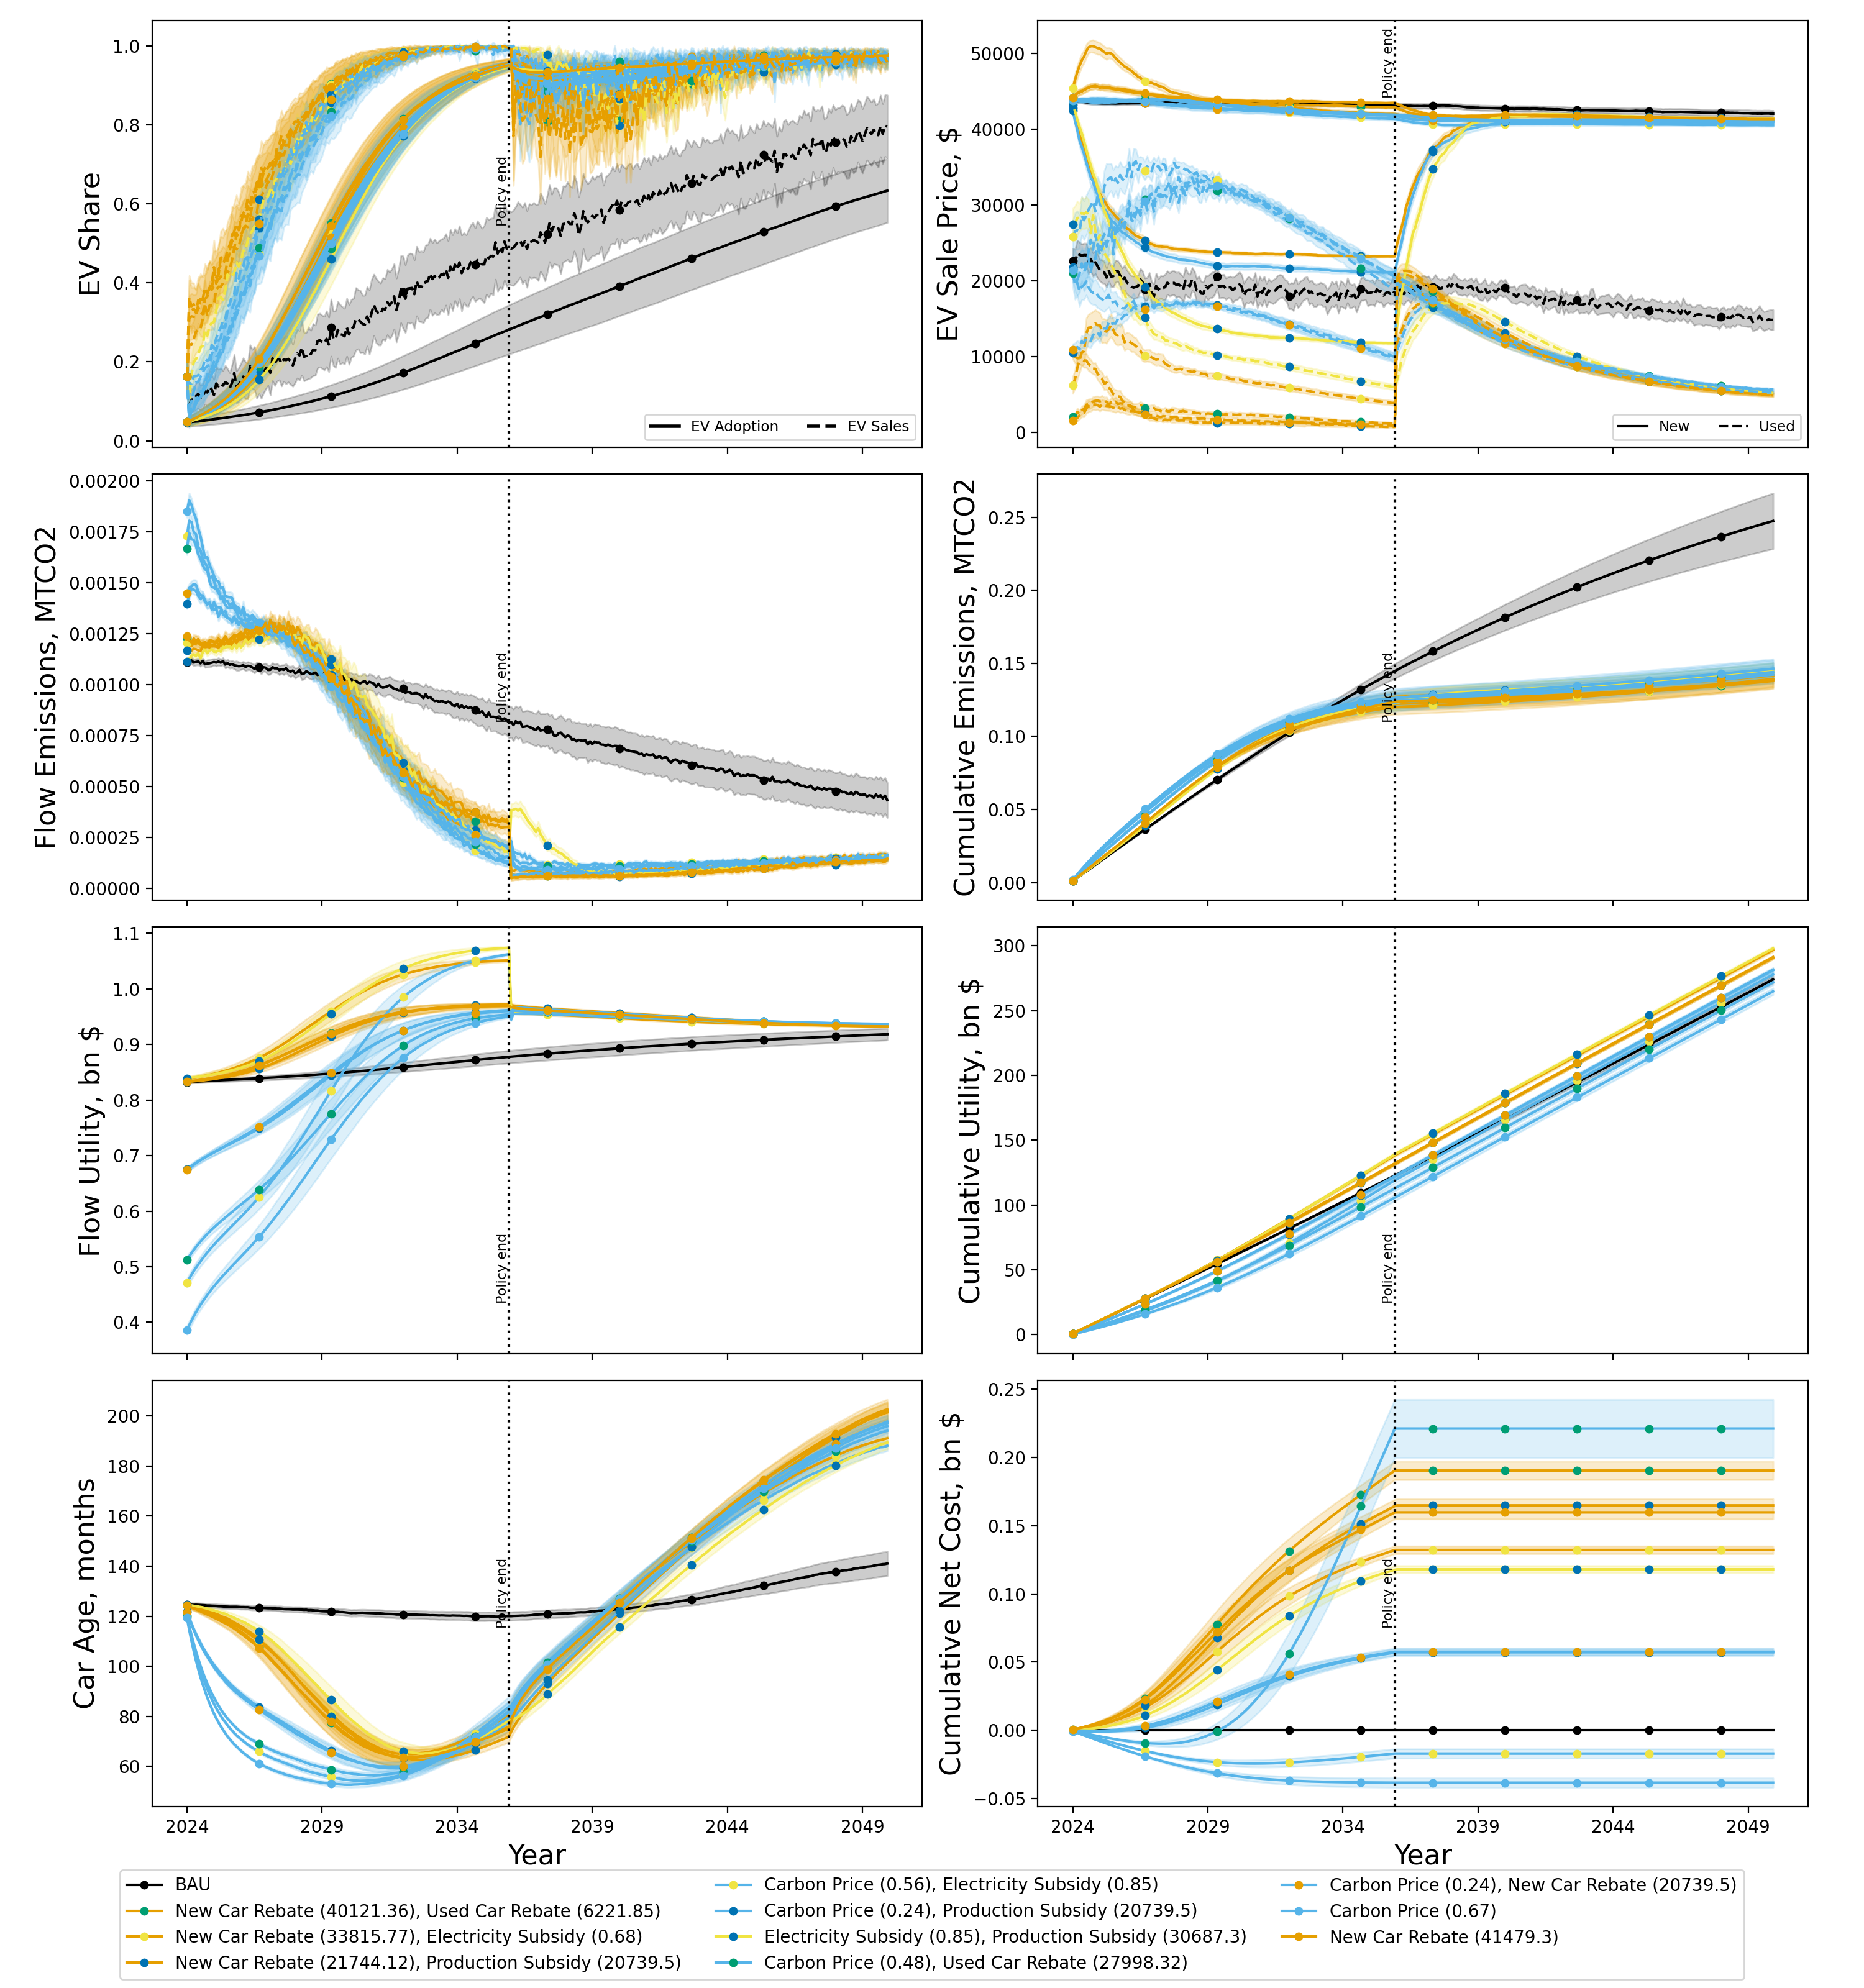
\includegraphics[width=0.9\linewidth]{Figure_5.png}
		\caption{Policy mix trajectories to 2050 with confidence intervals obtained over 64 Monte Carlo simulations.}
		\label{fig:policy_low_intensity}
	\end{figure}
    
	We remove the policy instruments in 2035 and run the projection until 2050 in order to verify that the policy-induced transition remains stable. The top left panel shows that, regardless of the policy used, EVs remain the preferred option after public intervention stops \textcolor{green}{after a short period of re-adjustment}. Furthermore, under the BAU scenario, uptake \textcolor{red}{slightly exceeds 40} \textcolor{green}{is near $60$}\% and the proportion of total sales \textcolor{red}{are 60} \textcolor{green}{is near 80}\% by 2050. This motivates the need for present-day bold policy interventions as a necessary transitional boost.
	
	The average retail price of EVs converges to a stable value once the policies are removed. The top right panel shows that the long-run average price of new and used EVs is lower than the BAU scenario for all transition policies. This is caused by two factors. First, the accelerated transition enables more research in EVs, leading to superior technologies. Second, because the entire population uses EVs, firms offer cheaper designs to satisfy low-income customers, whereas in the BAU scenario, EVs are targeted at high-spending segments. \textcolor{red}{Interestingly, in the case where the production subsidy and rebates for new EVs are implemented (dark blue and orange), the EV price is higher than in the other policy pairs after the incentives are removed. As indicated in the policy pairs analysis, rebates and production subsidies direct innovation towards other attributes than cost, thus creating a gap with respect to other policies after the instruments are removed.}   
	
	In the long-term, all emission flows converge to below the BAU due to the high EV uptake (see second row to the left of Figure \ref{fig:policy_low_intensity}). The removal of the incentives reduces the turnover of new cars and stabilises the production of new EVs. We observe a short-term bump in the transition led by electricity and production subsidies (yellow line and dark blue dots) after the incentives are removed. This is due to the combination of two policy-induced effects. First, the price adjustment after removing production subsidies is sluggish (top right panel), resulting in a post-policy transition period where EVs remain relatively cheap. Second, as discussed in the analysis of policy pairs, this combination directs technological change towards quality and battery size. After removing the electricity subsidy, users with large distance travelled switch to EVs with higher efficiency during the time-lapse of price adjustment, thus causing a transitional increase in production emissions.  
    
    \textcolor{red}{Except for the new EV rebates alone (orange) or combined with production subsidies (orange and dark blue), a} \textcolor{green}{A}ll policies achieve lower cumulative emissions than the BAU before \textcolor{red}{2044} \textcolor{green}{2035} (see second row to the right of Figure \ref{fig:policy_low_intensity}). \textcolor{green}{All transitions achieve statistically indistinguishable emission reduction levels accumulating about half than the emissions acrued in the BAU scenario.} {Table \ref{tab:emissions} displays the percentage change in emissions of each policy scenario in 2050 with respect to the BAU scenario in the same year. It can be observed that "carrot and stick" approaches (i.e. carbon price and a subsidy) achieve the highest reductions.    

    \begin{table}[h]
        \centering
        \caption{Cumulative Emissions Change Relative to BAU at Final Time Step}
        \label{tab:emissions}
        \begin{tabular}{lc}
            \toprule
            \textbf{Policy Combination} & \textbf{Change (\%)} \\
            \midrule
            New Car Rebate + Used Car Rebate & $-$44.23 \\
            New Car Rebate & $-$43.85 \\
            New Car Rebate + Electricity Subsidy & $-$43.71 \\
            New Car Rebate + Production Subsidy & $-$42.71 \\
            Carbon Price + New Car Rebate & $-$42.48 \\
            Carbon Price + Used Car Rebate & $-$41.78 \\
            Carbon Price + Production Subsidy & $-$41.69 \\
            Electricity Subsidy + Production Subsidy & $-$41.36 \\
            Carbon Price & $-$40.88 \\
            Carbon Price + Electricity Subsidy & $-$40.87 \\
            \bottomrule
        \end{tabular}
    \end{table}
}	
	During the \textcolor{red}{early policy period} \textcolor{green}{the first five years of the policy period}, the flow of utility of policy pairs including a carbon price (\textcolor{red}{green} \textcolor{green}{light blue lines}) is much lower than that of either the BAU or subsidy-only policies (see third row to the left of Figure \ref{fig:policy_low_intensity})\textcolor{red}{. Even in the best-case scenario, the yearly utility does not catch up to the BAU until 2031}, which may result in a period of sustained political pressure to roll back the carbon price due to its perceived economic burden. After 2035, consumer utility gradually declines \textcolor{green}{in all scenarios} due to the increasing age of the car fleet\textcolor{green}{,while in policies including an electricity subsidy there is a sizeable drop in utility after the policy is removed}. However, EVs remain a preferred alternative that yields higher consumer satisfaction, provided that the post-policy utility of transition scenarios exhibits higher yearly utility than the BAU scenario. In terms of cumulative utility (see third row to the right of Figure \ref{fig:policy_low_intensity}), only the carbon price (\textcolor{red}{green} \textcolor{green}{light blue lines and dots}) \textcolor{red}{and its combination with the used car rebate (green and light blue) do} \textcolor{green}{does} not surpass the BAU by 2050.
	
	The car age drops substantially with respect to the BAU scenario due to the renewal of the car fleet (see bottom left panel of Figure \ref{fig:policy_low_intensity}). However, after removing the policies, the average car age exceeds that of the BAU in all cases. This lower replacement rate is due to fact that EVs have higher efficiencies than their ICEVs counterparts. Thus, car users have little reason to buy new cars when used cars are of a high calibre. In addition to indicating higher satisfaction for EVs, the fact that EVs are kept for longer contributes to sustainability by lowering the manufacturing emissions. 
	
	\textcolor{red}{Policies including a carbon price (green) have a moderate net cost, having only the carbon price and its combination with electricity subsidies (green and yellow) with a net surplus (see bottom right panel of Figure \ref{fig:policy_low_intensity}). Conversely, the rebate to new EVs and its combination with a production subsidy (orange and dark blue) lead to substantial increases in policy costs due to overproduction and over-replacement of EVs. %Intermediate costs are found in all other combinations.} 
    \textcolor{green}{In analysing the cumulative net policy cost (bottom right panel), we identify two clusters of policy costs. Firstly, policies including a carbon price (light blue line), except when combined with a used car rebate (green dots), feature the lowest costs. When combined with an electricity subsidy (yellow dots) or used as a single policy (light blue dots) the tax revenues result in a net cumulative revenue. The carbon price reduces the cumulative cost of the adoption subsidy by two thirds. The rest of the policies range two to five times the cost of the carbon tax combined with the production subsidy.}
	
	From our simulation experiments, we derive several key results. First, policy combinations can improve the political feasibility of the EV transition by reducing the intensity of policies and minimising their induced negative impacts. \textcolor{red}{Counter-intuitively, the addition of supplementary policies to a carbon price can lower the temporary overshoot in production emissions whilst mitigating utility losses in the medium run at a relatively low cost. In the case of the rebate for new cars, some combinations reduce emissions with respect to the single policy and policy costs without substantially affecting utility. Furthermore, the pairing of production and electricity subsidies appears as a suitable alternative despite the fact that neither of the instruments can achieve a 95\% EV transition when applied in isolation.} \textcolor{green}{The inclusion of electricity subsidies, despite not meeting the 95\% target when implemented as a single policy, minimises, or fully mitigates, the transition risks of single policies. The highest emission reductions are achieved with the combination of a carbon price and electricity subsidy without incurring a net policy cost. The highest cumulative utility is achieved with the combination of a production and an electricity subsidy, while the net policy cost is reduced in comparison with the production subsidy alone.}
	
	A second takeaway we obtain from our results is that, before \textcolor{red}{2035} \textcolor{green}{2030}, all transition policies entail drawbacks. The required large-scale deployment of EVs causes an increase in manufacturing emissions that exceeds the savings in gasoline use. Furthermore, all policies lead to either losses in cumulative utility or net policy costs. Therefore, policymakers must allocate a budget to the EV transition or face political pushback on implemented policies.
	
	As a third point, in the long run and after removing the incentives, successful transitions remain stable, and the flows of each variable converge. In the aftermath, the transition to EVs leads to a scenario where EVs are cheaper and are kept for longer, consumers are more satisfied, and mobility is less polluting. 	
	
	\section{Conclusions} \label{Sec_concl}
	In the pursuit of light transportation decarbonization, this paper proposes an agent-based model (ABM) to examine the complex interplay between consumer adoption, firm innovation, and policy incentives in the transition to electric vehicles (EVs). We build upon previous literature studying EV transitions by analysing policy mixes in an ABM integrating discrete choice models, social influence dynamics, a used car market, endogenous pricing, and directed innovation through an NK framework. By integrating these submodules, we replicate the complex dynamics between car users and manufacturers that are key in the diffusion of innovations. The model is calibrated on the time frame of 2001-2023 in California, with a policy road map considered until 2035. Our study addresses the following research questions: 1) Can a combination of market-based policies lead to a medium-term technological transition in the automotive sector? 2) What policy-mix minimises transition costs in terms of public budget, consumer utility, and carbon emissions? 3) Can EV uptake be sustained after removing the policy incentives that caused it? 
	
	To answer these questions, we simulate a battery of policy instruments to fuel EV adoption, including a carbon price, an electricity and production subsidy, and a rebate for new and used EVs. When implementing single-policy packages, only the carbon price and the rebate for new EVs achieve the 95\% target uptake by 2035. However, each policy faces severe feasibility challenges due to the high policy intensities required. We identify the following policy trade-offs: the carbon price generates a surplus but causes a collapse in consumer utility, whilst the rebate for new EVs leads to large policy costs \textcolor{red}{and induces an overshoot in emissions due to the overproduction of new EVs}.
	
	In order to mitigate these downsides, we explore policy combinations involving two instruments. By introducing pairs of policies, the intensity and negative outcomes of the carbon price \textcolor{red}{or the new EV rebate} \textcolor{green}{the rebate for new EVs and the production subsidies} can be minimised. \textcolor{red}{Furthermore, the combination of production and electricity subsidies becomes an alternative to meet the uptake target despite their ineffectiveness when implemented in isolation.} These results highlight the importance of exploiting instrument complementarity when formulating policy packages in order to reduce policy trade-offs. Additionally, we find that \textcolor{red}{not all policy pairs produce positive synergies. In the case of a rebate for new cars and production subsidies, the results are simply greater policy costs and larger emissions with no increase in consumer utility} \textcolor{green}{some policy pairs lead to an absolute improvement in the three evaluated dimensions, indicating strong synergies}.
	
	To test the stability of the EV transition, we simulate the projections until 2050 after removing the incentives in 2035. Once the transition is consolidated, the system converges to a lower flow of emissions and higher utility regardless of the policies implemented to achieve the desired uptake. Ultimately, the widespread diffusion of EVs leads to lower car costs, longer lifespans, increased consumer satisfaction, and reduced pollution from mobility. Notably, combinations of carbon price and subsidies yield \textcolor{yellow}{30}\% reductions in cumulative emissions with respect to the BAU scenario.
    
	%%%%%%%%%%%%%%%%%%%%%%%%%%%%%%%%%%%%%%%%%%%%
    
	Looking ahead, the limitations of the model provide key areas for future research. A key shortcoming of the scaleability of this research is the lack of financial and physical constraints. Financial markets are a crucial institution for the large-scale adoption in EVs as they determine the ability of manufacturers to invest in R\&D and the required capital for EV production. Physical constraints also play an important role as they limit the speed of EV deployment due to the necessary build-up of productive infrastructure and car stocks. Future research should incorporate capital costs of switching production and a supply model with an explicit representation of production planning and inventory management.

    Incorporating more sophisticated forecasting techniques and factoring in expected regulation can crucially modify investment and purchase decisions. By doing so, policies such as standards and regulations could be assessed. Additionally, this would enable the study of more realistic time-varying carbon price implementations such as the EU-ETS.
    
    To better represent the role of pro-environmental attitudes or conspicuous consumption in purchasing behaviours. For example by expanding the representation of social learning beyond a threshold model to enrich car users with social norms and behavioural control such as in the Theory of Planned Behaviour \citep{ajzen1991theory}. This would facilitate the inclusion of policies such as information provision, media \citep{eppstein2011agent} or marketing that may affect purchasing behaviour by changing personal norms towards EVs. 
    
    The model contributes valuable insights into relative trends in policy mix effectiveness. However, translating these results into concrete recommendations would benefit from moving beyond calibration to validation. Achieving this requires a larger car user population to reduce noise in outputs and avoid overfitting of model parameters. Future research could support this through model parallelisation, enabling time-series data on EV fleet size or sales to be split into training, validation, and test sets.
    
    % Further positive synergies can be found by studying policy mixes including more than two instruments. In addition, other policies may be included in the analysis by improving upon limitations in the model where simplifications have been made. 
    

		
	%Future research could also incorporate the implications that EV production has on material dependence by endongeneizing the cost and emissions associated to the inputs required for EV production. This would allow studying the implications of innovation on material use efficiency as well as the inclusion of a carbon-border adjustment mechanism to price in imported production emissions.

    %%%%%%%%%%%%%%%%%%%%%%%%%%%%%%%%%%%%%%%%%%%%%%%%%%%
    
	%Given that the results of our simulations indicate that emission reductions, relative to the BAU scenario, are only achieved in the long-run, we endorse the study and implementation of alternative policies to minimise car dependence, in both use and ownership. This includes the promotion and improvement of public transport infrastructure, urban re-design aimed at reducing mobility needs, or car sharing schemes to lower car ownership. Moreover, future research should address the price responsiveness car users have in their driving choices. The simultaneous study of urban design to reduce car dependence and price responsiveness in mileage is a promising research avenue as the distance driven becomes more elastic when car mobility needs are minimised. 
	
	%The absence of sophisticated expectation formation, financial constraints, and supply chain dynamics means that our analysis does not fully capture real world barriers to rapid EV deployment. Crucially, our findings reinforce that a singular focus on replacing internal combustion engine vehicles with electric vehicles is insufficient to achieve deep decarbonization of transport due to persistent production emissions. Policies must also target the root of the problem: an over-reliance on private car ownership and use.
	
	As a final note, policymakers must apply more stringent policies in order to achieve a quick transition to EVs with cleaner mobility. We strongly encourage exploiting positive synergies between policy instruments to improve the political acceptability of the policy and minimise transitional costs. Critically, our study highlights the relevance of system co-evolution when evaluating policies to anticipate the multi-dimensional risks embedded in technological change.  %However, our study demonstrates that a fast and ambitious reduction in carbon emissions requires tackling the root of the problem: an over-reliance on private car ownership and use.   
	

	\section*{Declaration of Interest Statement}
	This work has received funding from the European Union’s Horizon 2020 research and innovation programme under the Marie Skłodowska-Curie grant agreement No 956107, "Economic Policy in Complex Environments (EPOC)". We thank Herbert David, Jeroen van den Bergh and Ivan Savin for their insightful and constructive critisim of early versions of the manuscript. We are grateful to the reviewers for their comments and suggestions that greatly improved the quality of the manuscript.
	
	\section*{Code availability statement}
	The model code, data and documentation are available at \href{https://github.com/danielTorren/Driving-in-the-wrong-direction.git}{github.com/danielTorren/Driving-in-the-wrong-direction.git}.

	%%%%%%%%%%%%%%%%%%%%%%%%%%%%%%%%%%%%%%%%%%%%%%%%%%%%%%%%%%%%%%%%%%%%%
	%\printbibliography
	\begin{thebibliography}{}

\bibitem[{360 Research Reports}, 2026]{360ResearchReports2026UsedCars}
{360 Research Reports} (2026).
\newblock Used cars market size, share, growth, and industry analysis, by type
  (commercial vehicles, passenger cars), by application (online transactions,
  offline transactions), regional insights and forecast to 2035.
\newblock Market research report, 360 Research Reports.
\newblock Accessed: 2026-04-01.

\bibitem[Abas and Tan, 2024]{abas2024modeling}
Abas, P.~E. and Tan, B. (2024).
\newblock Modeling the impact of different policies on electric vehicle
  adoption: An investigative study.
\newblock {\em World Electric Vehicle Journal}, 15(2):52.
\newblock Open access.

\bibitem[Aghion, 2019]{aghion2019path}
Aghion, P. (2019).
\newblock Path dependence, innovation and the economics of climate change.
\newblock In Fouquet, R., editor, {\em Handbook on Green Growth}, pages 67--83.
  Edward Elgar Publishing, Cheltenham, UK.

\bibitem[Ajzen, 1991]{ajzen1991theory}
Ajzen, I. (1991).
\newblock The theory of planned behavior.
\newblock {\em Organizational behavior and human decision processes},
  50(2):179--211.

\bibitem[Anderson et~al., 2013]{Anderson2013}
Anderson, S.~T., Kellogg, R., and Sallee, J.~M. (2013).
\newblock What do consumers believe about future gasoline prices?
\newblock {\em Journal of Environmental Economics and Management},
  66(3):383--403.

\bibitem[Axsen and Kurani, 2013]{axsen2013vehicles}
Axsen, J. and Kurani, K.~S. (2013).
\newblock Hybrid, plug-in hybrid, or electric---{What} do car buyers want?
\newblock {\em Energy Policy}, 61:532--543.

\bibitem[Bakker and Trip, 2013]{Bakker2013Policy}
Bakker, S. and Trip, J.~J. (2013).
\newblock Policy options to support the adoption of electric vehicles in the
  urban environment.
\newblock {\em Transportation Research Part D: Transport and Environment},
  25:18--23.

\bibitem[Bassart-i Loré, 2026]{bassart2026mixing}
Bassart-i Loré, M. (2026).
\newblock Mixing innovation policies for low-carbon transitions? an agent-based
  approach.
\newblock {\em Technological Forecasting and Social Change}, 222:124372.

\bibitem[Baumann and Siggelkow, 2013]{baumann_siggelkow_2013}
Baumann, O. and Siggelkow, N. (2013).
\newblock Dealing with complexity: Integrated vs. chunky search processes.
\newblock {\em Organization Science}, 24(1):116--132.

\bibitem[Beiser-McGrath et~al., 2023]{Beiser-McGrath2023}
Beiser-McGrath, L.~F., Bernauer, T., and Prakash, A. (2023).
\newblock Command and control or market-based instruments? public support for
  policies to address vehicular pollution in beijing and new delhi.
\newblock {\em Environmental Politics}, 32(4):586--618.

\bibitem[Bilal and K{\"a}nzig, 2024]{bilal2024macroeconomic}
Bilal, A. and K{\"a}nzig, D.~R. (2024).
\newblock The macroeconomic impact of climate change: Global vs. local
  temperature.
\newblock Technical report, National Bureau of Economic Research.

\bibitem[Biresselioglu et~al., 2018]{biresselioglu_electric_2018}
Biresselioglu, M., Kaplan, M., and Yilmaz, B. (2018).
\newblock Electric mobility in europe: A comprehensive review of motivators and
  barriers in decision making processes.
\newblock {\em Transportation Research Part A: Policy and Practice}, 109:1--13.

\bibitem[Borlaug et~al., 2023]{borlaug_public_2023}
Borlaug, B., Yang, F., Pritchard, E., Wood, E., and Gonder, J. (2023).
\newblock Public electric vehicle charging station utilization in the united
  states.
\newblock {\em Transportation Research Part D: Transport and Environment},
  114:103564.

\bibitem[Bouma et~al., 2019]{bouma2019policy}
Bouma, J.~A., Verbraak, M., Dietz, F., and Brouwer, R. (2019).
\newblock Policy mix: mess or merit?
\newblock {\em Journal of Environmental Economics and Policy}, 8(1):32--47.

\bibitem[Broadbent et~al., 2022]{Broadbent2022Accelerating}
Broadbent, G.~H., Allen, C.~I., Wiedmann, T., and Metternicht, G.~I. (2022).
\newblock Accelerating electric vehicle uptake: Modelling public policy options
  on prices and infrastructure.
\newblock {\em Transportation Research Part A: Policy and Practice},
  162:155--174.

\bibitem[Burra et~al., 2024]{burra_free-ridership_2024}
Burra, L.~T., Sommer, S., and Vance, C. (2024).
\newblock Free-ridership in subsidies for company- and private electric
  vehicles.
\newblock {\em Energy Economics}, 131:107333.

\bibitem[Busse et~al., 2013]{busse2013consumers}
Busse, M.~R., Knittel, C.~R., and Zettelmeyer, F. (2013).
\newblock Are consumers myopic? evidence from new and used car purchases.
\newblock {\em American Economic Review}, 103(1):220--256.

\bibitem[{California Air Resources Board}, 1990a]{CARB1990LEV}
{California Air Resources Board} (1990a).
\newblock Final regulation order. low-emission vehicles and clean fuels.
  california exhaust emission standards and test procedures for 1988 and
  subsequent model passenger cars, light-duty trucks, and medium-duty vehicles.
\newblock Technical report, California Air Resources Board.

\bibitem[{California Air Resources Board}, 1990b]{CARB1990proposed}
{California Air Resources Board} (1990b).
\newblock Proposed regulations for low-emission vehicles and clean fuels: Final
  statement of reasons.
\newblock Technical report, California Air Resources Board.

\bibitem[{California Air Resources Board}, 1990c]{CARB1990hearing}
{California Air Resources Board} (1990c).
\newblock Transcripts of public hearing, september 27 and 28.

\bibitem[Cannavacciuolo et~al., 2025]{cannavacciuolo_agent-based_2025}
Cannavacciuolo, L., Maione, V., Ponsiglione, C., and Primario, S. (2025).
\newblock Agent-based modelling of electric vehicle adoption: A
  multidimensional perspective assessment.
\newblock {\em Research in Transportation Business \& Management}, 61:101407.

\bibitem[Cohen and Levinthal, 1990]{cohen1990absorptive}
Cohen, W.~M. and Levinthal, D.~A. (1990).
\newblock Absorptive capacity: A new perspective on learning and innovation.
\newblock {\em Administrative Science Quarterly}, 35:128--152.

\bibitem[Cranmer et~al., 2020]{cranmer2020frontier}
Cranmer, K., Brehmer, J., and Louppe, G. (2020).
\newblock The frontier of simulation-based inference.
\newblock {\em Proceedings of the National Academy of Sciences},
  117(48):30055--30062.

\bibitem[Destek et~al., 2025]{destek_market-based_2025}
Destek, M.~A., {\"O}zkan, O., and Tiwari, S. (2025).
\newblock Market-based and non-market-based policies: A quantile approach to
  environmental technology innovation in g-7 countries.
\newblock {\em Technological Forecasting and Social Change}, 217:124173.

\bibitem[Dijk et~al., 2013]{dijk2013incorporating}
Dijk, M., Kemp, R., and Valkering, P. (2013).
\newblock Incorporating social context and co-evolution in an innovation
  diffusion model—with an application to cleaner vehicles.
\newblock {\em Journal of Evolutionary Economics}, 23(2):295--329.

\bibitem[Domarchi and Cherchi, 2023]{domarchi2023electric}
Domarchi, C. and Cherchi, E. (2023).
\newblock Electric vehicle forecasts: a review of models and methods including
  diffusion and substitution effects.
\newblock {\em Transport reviews}, 43(6):1118--1143.

\bibitem[Dosi et~al., 2010]{Dosi2010}
Dosi, G., Fagiolo, G., and Roventini, A. (2010).
\newblock Schumpeter meeting keynes: A policy-friendly model of endogenous
  growth and business cycles.
\newblock {\em Journal of Economic Dynamics and Control}, 34(9):1748--1767.

\bibitem[Dyer et~al., 2024]{dyer2024black}
Dyer, J., Cannon, P., Farmer, J.~D., and Schmon, S.~M. (2024).
\newblock Black-box bayesian inference for agent-based models.
\newblock {\em Journal of Economic Dynamics and Control}, 161:104827.

\bibitem[Eggers and Eggers, 2011]{EGGERS201151}
Eggers, F. and Eggers, F. (2011).
\newblock Where have all the flowers gone? forecasting green trends in the
  automobile industry with a choice-based conjoint adoption model.
\newblock {\em Technological Forecasting and Social Change}, 78(1):51--62.

\bibitem[Eppstein et~al., 2011]{eppstein2011agent}
Eppstein, M.~J., Grover, D.~K., Marshall, J.~S., and Rizzo, D.~M. (2011).
\newblock An agent-based model to study market penetration of plug-in hybrid
  electric vehicles.
\newblock {\em Energy Policy}, 39(6):3789--3802.

\bibitem[Fadiran et~al., 2020]{Fadiran2020Review}
Fadiran, G., Rogan, F., Mulholland, E., and O'Gallachoir, B. (2020).
\newblock Agent based models to understand diffusion of low carbon road
  transport technologies: a review of application and approaches.
\newblock {\em SSRN}, (3702784).

\bibitem[Fan and Li, 2025]{fan2025unfolding}
Fan, X. and Li, C. (2025).
\newblock "to be unfolding" or "be on its last legs"—preferential tax
  policies between supply and demand and the development of the new energy
  vehicle industry based on an abm model.
\newblock {\em Energy Policy}, 200:114552.

\bibitem[fei Chen et~al., 2019]{chen_assessing_2019}
fei Chen, C., de~Rubens, G.~Z., Noel, L., Kester, J., and Sovacool, B.~K.
  (2019).
\newblock Assessing the socio-demographic, technical, economic and behavioral
  factors of nordic electric vehicle adoption and the influence of
  vehicle-to-grid preferences.
\newblock {\em Renewable and Sustainable Energy Reviews}, 121:109692.

\bibitem[Feng et~al., 2019]{FENG2019196}
Feng, B., Ye, Q., and Collins, B.~J. (2019).
\newblock A dynamic model of electric vehicle adoption: The role of social
  commerce in new transportation.
\newblock {\em Information \& Management}, 56(2):196--212.
\newblock Social Commerce and Social Media: Behaviors in the New Service
  Economy.

\bibitem[Ferguson et~al., 2018]{FERGUSON2018208}
Ferguson, M., Mohamed, M., Higgins, C.~D., Abotalebi, E., and Kanaroglou, P.
  (2018).
\newblock How open are canadian households to electric vehicles? a national
  latent class choice analysis with willingness-to-pay and metropolitan
  characterization.
\newblock {\em Transportation Research Part D: Transport and Environment},
  58:208--224.

\bibitem[Gebhardt et~al., 2026]{Gebhardt2026}
Gebhardt, S., Hou, Y., and Yarime, M. (2026).
\newblock Directing environmental innovation toward radical clean technologies
  for sustainable transitions: Market-based vs. command-and-control policies.
\newblock {\em Research Policy}, 55(4):105446.

\bibitem[Givoni et~al., 2013]{givoni_policy_2013}
Givoni, M., Macmillen, J., Banister, D., and Feitelson, E. (2013).
\newblock From policy measures to policy packages.
\newblock {\em Transport Reviews}, 33(1):1--20.

\bibitem[Greene, 2010]{greene2010consumers}
Greene, D.~L. (2010).
\newblock How consumers value fuel economy: A literature review.

\bibitem[Greene et~al., 2014]{greene2014public}
Greene, D.~L., Park, S., and Liu, C. (2014).
\newblock Public policy and the transition to electric drive vehicles in the
  us: The role of the zero emission vehicles mandates.
\newblock {\em Energy Strategy Reviews}, 5:66--77.

\bibitem[Grieco et~al., 2024]{Grieco2024MarketPower}
Grieco, P. L.~E., Murry, C., and Yurukoglu, A. (2024).
\newblock The evolution of market power in the u.s. automobile industry.
\newblock {\em The Quarterly Journal of Economics}, 139(2):1201--1253.

\bibitem[Guven et~al., 2026]{guven2026assessing}
Guven, D., Kayalica, M.~O., and Bozdag, C.~E. (2026).
\newblock Assessing policy interventions for electric vehicle adoption through
  an agent-based environmental framework.
\newblock {\em Applied Energy}, 407:127338.

\bibitem[Hardman, 2019]{Hardman2019Understanding}
Hardman, S. (2019).
\newblock Understanding the impact of reoccurring and non-financial incentives
  on plug-in electric vehicle adoption---a review.
\newblock {\em Transportation Research Part A: Policy and Practice}, 119:1--14.

\bibitem[Hardman et~al., 2017]{HARDMAN2017EVRebate}
Hardman, S., Chandan, A., Tal, G., and Turrentine, T. (2017).
\newblock The effectiveness of financial purchase incentives for battery
  electric vehicles – a review of the evidence.
\newblock {\em Renewable and Sustainable Energy Reviews}, 80:1100--1111.

\bibitem[He et~al., 2020]{he2020integration}
He, B.-J., Zhao, D., and Gou, Z. (2020).
\newblock Integration of low-carbon eco-city, green campus and green building
  in china.
\newblock In Gou, Z., editor, {\em Green Building in Developing Countries},
  pages 49--78. Springer, Cham, Switzerland.

\bibitem[Head et~al., 2021]{head_2021_5565057}
Head, T., Kumar, M., Nahrstaedt, H., Louppe, G., and Shcherbatyi, I. (2021).
\newblock scikit-optimize/scikit-optimize.

\bibitem[Helm et~al., 2003]{helm2003credible}
Helm, D., Hepburn, C., and Mash, R. (2003).
\newblock Credible carbon policy.
\newblock {\em Oxford Review of Economic Policy}, 19(3):438--450.

\bibitem[Herrmann and Savin, 2017]{herrmann2017optimal}
Herrmann, J. and Savin, I. (2017).
\newblock Optimal policy identification: Insights from the german electricity
  market.
\newblock {\em Technological Forecasting \& Social Change}, 122:71--90.

\bibitem[Hidrue et~al., 2011]{hidrue2011willingness}
Hidrue, M.~K., Parsons, G.~R., Kempton, W., and Gardner, M.~P. (2011).
\newblock Willingness to pay for electric vehicles and their attributes.
\newblock {\em Resource and energy economics}, 33(3):686--705.

\bibitem[Hulshof and Mulder, 2020]{hulshof2020willingness}
Hulshof, D. and Mulder, M. (2020).
\newblock Willingness to pay for {CO2} emission reductions in passenger car
  transport.
\newblock {\em Environmental and Resource Economics}, 75:899--929.

\bibitem[Jaffe and Palmer, 1997]{jaffe_environmental_1997}
Jaffe, A.~B. and Palmer, K. (1997).
\newblock Environmental regulation and innovation: A panel data study.
\newblock {\em The Review of Economics and Statistics}, 79(4):610--619.

\bibitem[Jain and Kogut, 2014]{jain2014memory}
Jain, A. and Kogut, B. (2014).
\newblock Memory and organizational evolvability in a neutral landscape.
\newblock {\em Organization Science}, 25(2):479--493.

\bibitem[Jang and Choi, 2021]{jang2021vehicles}
Jang, S. and Choi, J.~Y. (2021).
\newblock Which consumer attributes will act crucial roles for the fast market
  adoption of electric vehicles?: {Estimation} on the asymmetrical \&
  heterogeneous consumer preferences on the {EVs}.
\newblock {\em Energy Policy}, 156:112469.

\bibitem[Jaramillo et~al., 2022]{ipcc2022transport}
Jaramillo, P., Kahn~Ribeiro, S., Newman, P., Dhar, S., Diemuodeke, O.~E.,
  Kajino, T., Lee, D.~S., Nugroho, S.~B., Ou, X., Hammer~Strømman, A., and
  Whitehead, J. (2022).
\newblock Transport.
\newblock In Shukla, P.~R., Skea, J., Slade, R., Al~Khourdajie, A., van Diemen,
  R., McCollum, D., Pathak, M., Some, S., Vyas, P., Fradera, R., Belkacemi, M.,
  Hasija, A., Lisboa, G., Luz, S., and Malley, J., editors, {\em Climate Change
  2022: Mitigation of Climate Change}, Contribution of Working Group III to the
  Sixth Assessment Report of the Intergovernmental Panel on Climate Change,
  chapter~10. Cambridge University Press, Cambridge, UK and New York, NY, USA.

\bibitem[Juntunen and Shakeel, 2026]{Juntunen2026}
Juntunen, J.~K. and Shakeel, S.~R. (2026).
\newblock Contextualizing policy mixes – a configurational study on rapid
  transitions.
\newblock {\em Research Policy}, 55(1):105359.

\bibitem[Kauffman, 1993]{kauffman1993origins}
Kauffman, S.~A. (1993).
\newblock {\em The Origins of Order: Self-Organization and Selection in
  Evolution}.
\newblock Oxford University Press, New York.

\bibitem[Keyes and Crawford-Brown, 2018]{keyes2018vehicles}
Keyes, A.~K. and Crawford-Brown, D. (2018).
\newblock The changing influences on commuting mode choice in urban {England}
  under {Peak Car}: {A} discrete choice modelling approach.
\newblock {\em Transportation Research Part F: Traffic Psychology and
  Behaviour}, 58:167--176.

\bibitem[Kiesling et~al., 2012]{Kiesling2012}
Kiesling, E., G{\"u}nther, M., Stummer, C., and Wakolbinger, L.~M. (2012).
\newblock Agent-based simulation of innovation diffusion: a review.
\newblock {\em Central European Journal of Operations Research},
  20(2):183--230.

\bibitem[Kollmuss and Agyeman, 2002]{kollmuss2002mind}
Kollmuss, A. and Agyeman, J. (2002).
\newblock Mind the gap: why do people act environmentally and what are the
  barriers to pro-environmental behavior?
\newblock {\em Environmental education research}, 8(3):239--260.

\bibitem[Konc et~al., 2021]{konc2021social}
Konc, T., Savin, I., and van~den Bergh, J.~C. (2021).
\newblock The social multiplier of environmental policy: Application to carbon
  taxation.
\newblock {\em Journal of Environmental Economics and Management}, 105:102396.

\bibitem[K{\"o}nig et~al., 2021]{konig2021overview}
K{\"o}nig, A., Nicoletti, L., Schr{\"o}der, D., Wolff, S., Waclaw, A., and
  Lienkamp, M. (2021).
\newblock An overview of parameter and cost for battery electric vehicles.
\newblock {\em World Electric Vehicle Journal}, 12(1):21.

\bibitem[Kotler, 1989]{kotler1989mass}
Kotler, P. (1989).
\newblock From mass marketing to mass customization.
\newblock {\em Planning Review}, 17(5):10--47.

\bibitem[Kwon et~al., 2018]{Kwon2018Evaluation}
Kwon, Y., Son, S., and Jang, K. (2018).
\newblock Evaluation of incentive policies for electric vehicles: An
  experimental study on jeju island.
\newblock {\em Transportation Research Part A: Policy and Practice},
  116:404--412.

\bibitem[Langbroek et~al., 2016]{langbroek_effect_2016}
Langbroek, J.~H., Franklin, J.~P., and Susilo, Y.~O. (2016).
\newblock The effect of policy incentives on electric vehicle adoption.
\newblock {\em Energy Policy}, 94:94--103.

\bibitem[Ledna et~al., 2022]{ledna2022support}
Ledna, C., Muratori, M., Brooker, A., Wood, E., and Greene, D. (2022).
\newblock How to support ev adoption: Tradeoffs between charging infrastructure
  investments and vehicle subsidies in california.
\newblock {\em Energy Policy}, 165:112931.

\bibitem[Lee and Brown, 2021]{lee2021evaluating}
Lee, R. and Brown, S. (2021).
\newblock Evaluating the role of behavior and social class in electric vehicle
  adoption and charging demands.
\newblock {\em Iscience}, 24(8).

\bibitem[Levinthal, 1997]{levinthal1997adaptation}
Levinthal, D.~A. (1997).
\newblock Adaptation on rugged landscapes.
\newblock {\em Management Science}, 43(7):934--950.

\bibitem[Li et~al., 2019]{li2019evolutionary}
Li, J., Jiao, J., and Tang, Y. (2019).
\newblock An evolutionary analysis on the effect of government policies on
  electric vehicle diffusion in complex network.
\newblock {\em Energy policy}, 129:1--12.

\bibitem[Lodhia et~al., 2024]{Lodhia2024Assessment}
Lodhia, S.~K., Rice, J., Rice, B., and Martin, N. (2024).
\newblock Assessment of electric vehicle adoption policies and practices in
  australia: Stakeholder perspectives.
\newblock {\em Journal of Cleaner Production}, 446:141300.

\bibitem[Lynn, 2012]{lynn2012segmenting}
Lynn, M. (2012).
\newblock Segmenting and targeting your market: Strategies and limitations.
\newblock In {\em The Cornell School of Hotel Administration on Hospitality:
  Cutting Edge Thinking and Practice}, pages 351--369. John Wiley \& Sons.

\bibitem[Maestre-Andr{\'e}s et~al., 2019]{maestre-andres_perceived_2019}
Maestre-Andr{\'e}s, S., Drews, S., and Bergh, J. V.~D. (2019).
\newblock Perceived fairness and public acceptability of carbon pricing: a
  review of the literature.
\newblock {\em Climate Policy}, 19(9):1186--1204.

\bibitem[Malerba et~al., 2008]{MALERBA2008355}
Malerba, F., Nelson, R., Orsenigo, L., and Winter, S. (2008).
\newblock Public policies and changing boundaries of firms in a
  "history-friendly" model of the co-evolution of the computer and
  semiconductor industries.
\newblock {\em Journal of Economic Behavior \& Organization}, 67(2):355--380.
\newblock Agent-based models for economic policy design.

\bibitem[Maybury et~al., 2022]{Maybury2022ReviewEV}
Maybury, L., Corcoran, P., and Cipcigan, L. (2022).
\newblock Mathematical modelling of electric vehicle adoption: A systematic
  literature review.
\newblock {\em Transportation Research Part D: Transport and Environment},
  107:103278.

\bibitem[Mayol and Porcher, 2025]{mayol_analysis_2025}
Mayol, A. and Porcher, S. (2025).
\newblock Analysis of the determinants of support and participation in carbon
  tax riots in france.
\newblock {\em Applied Economics}, 57(15):1784--1802.

\bibitem[Mazzucato, 2013]{mazzucato2013financing}
Mazzucato, M. (2013).
\newblock Financing innovation: creative destruction vs. destructive creation.
\newblock {\em Industrial and Corporate Change}, 22(4):851--867.

\bibitem[Mazzucato and Semieniuk, 2017]{mazzucato2017public}
Mazzucato, M. and Semieniuk, G. (2017).
\newblock Public financing of innovation: New questions.
\newblock {\em Oxford Review of Economic Policy}, 33(1):24--48.

\bibitem[McCollum et~al., 2018]{mccollum_interaction_2018}
McCollum, D.~L., Wilson, C., Bevione, M., Carrara, S., Edelenbosch, O.~Y.,
  Emmerling, J., Guivarch, C., Karkatsoulis, P., Krey, V., Lin, Z., Broin, E.,
  Soim, S., van Vuuren, D.~P., Wicke, B., and Riahi, K. (2018).
\newblock Interaction of consumer preferences and climate policies in the
  global transition to low-carbon vehicles.
\newblock {\em Nature Energy}, 3:664--673.

\bibitem[McCoy and Lyons, 2014]{mccoy2014consumer}
McCoy, D. and Lyons, S. (2014).
\newblock Consumer preferences and the influence of networks in electric
  vehicle diffusion: An agent-based microsimulation in ireland.
\newblock {\em Energy Research \& Social Science}, 3:89--101.

\bibitem[McFadden, 1974]{McFadden1974}
McFadden, D. (1974).
\newblock Conditional logit analysis of qualitative choice behavior.
\newblock In Zarembka, P., editor, {\em Economic Theory and Mathematical
  Economics}, pages 105--142. Academic Press, New York, NY.

\bibitem[Mehdizadeh et~al., 2022]{mehdizadeh2022systematic}
Mehdizadeh, M., Nordfjaern, T., and Kl{\"o}ckner, C.~A. (2022).
\newblock A systematic review of the agent-based modelling/simulation paradigm
  in mobility transition.
\newblock {\em Technological Forecasting and Social Change}, 184:122011.

\bibitem[Metcalf, 2009]{metcalf_market-based_2009}
Metcalf, G.~E. (2009).
\newblock Market-based policy options to control {US} greenhouse gas emissions.
\newblock {\em Journal of Economic Perspectives}, 23(2):5--27.

\bibitem[Moore et~al., 2024]{moore2024synthesis}
Moore, F.~C., Drupp, M.~A., Rising, J., Dietz, S., Rudik, I., and Wagner, G.
  (2024).
\newblock Synthesis of evidence yields high social cost of carbon due to
  structural model variation and uncertainties.
\newblock {\em Proceedings of the National Academy of Sciences},
  121(52):e2410733121.

\bibitem[Muehlegger and Rapson, 2019]{Muehlegger2018Understanding}
Muehlegger, E. and Rapson, D. (2019).
\newblock Understanding the distributional impacts of vehicle policy: Who buys
  new and used alternative vehicles?
\newblock Technical report, National Center for Sustainable Transportation, UC
  Davis.

\bibitem[Nelson and Winter, 1977]{nelson1977search}
Nelson, R.~R. and Winter, S.~G. (1977).
\newblock In search of useful theory of innovation.
\newblock {\em Research Policy}, 6(1):36--76.

\bibitem[Neves et~al., 2019]{neves_technological_2019}
Neves, S., Marques, A., and Fuinhas, J. (2019).
\newblock Technological progress and other factors behind the adoption of
  electric vehicles: Empirical evidence for eu countries.
\newblock {\em Research in Transportation Economics}, 74:28--39.

\bibitem[Ning et~al., 2020]{ning2020incorporating}
Ning, W., Guo, J., Liu, X., and Pan, H. (2020).
\newblock Incorporating individual preference and network influence on choice
  behavior of electric vehicle sharing using agent-based model.
\newblock {\em International Journal of Sustainable Transportation},
  14(12):917--931.

\bibitem[Nuñez-Jimenez et~al., 2022]{nunez2022beyond}
Nuñez-Jimenez, A., Knoeri, C., Hoppmann, J., and Hoffmann, V.~H. (2022).
\newblock Beyond innovation and deployment: Modeling the impact of
  technology-push and demand-pull policies in germany's solar policy mix.
\newblock {\em Research Policy}, 51:104585.

\bibitem[{OECD}, 2025]{OECD2025Subsidies}
{OECD} (2025).
\newblock How subsidies shape global car and ev production.
\newblock Technical Report~14, OECD Publishing, Paris.

\bibitem[Ojeda-Diaz et~al., 2026]{ojeda-diaz_un-intended_2026}
Ojeda-Diaz, A.~J., Krueger, R., Jensen, A.~F., and Haustein, S. (2026).
\newblock The (un-)intended consequences of transport electrification: a
  scoping review of rebound and spillover effects.
\newblock {\em Transport Reviews}, 46(1):77--108.

\bibitem[{\O}stli et~al., 2017]{ostli2017generic}
{\O}stli, V., Fridstr{\o}m, L., Johansen, K.~W., and Tseng, Y.-Y. (2017).
\newblock A generic discrete choice model of automobile purchase.
\newblock {\em European Transport Research Review}, 9(1):16.

\bibitem[Pandita et~al., 2024]{pandita2024electrifying}
Pandita, D., Bhatt, V., Kumar, V., Fatma, A., and Vapiwala, F. (2024).
\newblock Electrifying the future: analysing the determinants of electric
  vehicle adoption.
\newblock {\em International Journal of Energy Sector Management},
  18(6):1767--1786.

\bibitem[Papamakarios and Murray, 2016]{papamakarios2016fast}
Papamakarios, G. and Murray, I. (2016).
\newblock Fast $\varepsilon$-free inference of simulation models with bayesian
  conditional density estimation.
\newblock {\em Advances in neural information processing systems}, 29.

\bibitem[Park et~al., 2018]{park_understanding_2018}
Park, E., Lim, J., and Cho, Y. (2018).
\newblock Understanding the emergence and social acceptance of electric
  vehicles as next-generation models for the automobile industry.
\newblock {\em Sustainability}, 10(3):662.

\bibitem[Peng and Bai, 2024]{peng2024identifying}
Peng, Y. and Bai, X. (2024).
\newblock Identifying social tipping point through perceived peer effect.
\newblock {\em Environmental Innovation and Societal Transitions}, 51:100847.
\newblock Volume 51, June 2024, 100847.

\bibitem[Piñas et~al., 2025]{moralejo_pinas_electric_2025}
Piñas, J.~M., Martinez-Gil, F., Santacruz, M.~S., and Fernández, F. (2025).
\newblock Electric vehicle market dynamics: A multi-agent approach to policy,
  infrastructure, and consumer behavior.
\newblock {\em Energy Policy}, 206:114800.

\bibitem[Puranam et~al., 2015]{Puranam2015}
Puranam, P., Stieglitz, N., Osman, M., and Pillutla, M.~M. (2015).
\newblock Modelling bounded rationality in organizations: Progress and
  prospects.
\newblock {\em Acad. Manag. Ann.}, 9(1):337--392.

\bibitem[Rasouli and Timmermans, 2016]{rasouli_influence_2016}
Rasouli, S. and Timmermans, H. (2016).
\newblock Influence of social networks on latent choice of electric cars: a
  mixed logit specification using experimental design data.
\newblock {\em Networks and Spatial Economics}, 16(1):99--130.

\bibitem[Rivkin, 2000]{rivkin_2000}
Rivkin, J.~W. (2000).
\newblock Imitation of complex strategies.
\newblock {\em Management Science}, 46(6):824--844.

\bibitem[Rogers, 2003]{rogers2003diffusion}
Rogers, E.~M. (2003).
\newblock {\em Diffusion of Innovations}.
\newblock Free Press, New York, 5 edition.

\bibitem[Savin et~al., 2022]{savin2022agent}
Savin, I., Creutzig, F., Filatova, T., Foramitti, J., Konc, T., Niamir, L.,
  Safarzynska, K., and van~den Bergh, J. (2022).
\newblock Agent-based modeling to integrate elements from different disciplines
  for ambitious climate policy.
\newblock {\em Wiley Interdisciplinary Reviews: Climate Change}, page e811.

\bibitem[Savin et~al., 2024]{savin2024carbon}
Savin, I., Drews, S., and van~den Bergh, J. (2024).
\newblock Carbon pricing--perceived strengths, weaknesses and knowledge gaps
  according to a global expert survey.
\newblock {\em Environmental Research Letters}, 19(2):024014.

\bibitem[Schloter, 2022]{SCHLOTER20222Depreciation}
Schloter, L. (2022).
\newblock Empirical analysis of the depreciation of electric vehicles compared
  to gasoline vehicles.
\newblock {\em Transport Policy}, 126:268--279.

\bibitem[Schmuch et~al., 2018]{Schmuch2018}
Schmuch, R., Wagner, R., H\"{o}rpel, G., Placke, T., and Winter, M. (2018).
\newblock Performance and cost of materials for lithium-based rechargeable
  automotive batteries.
\newblock {\em Nature Energy}, 3:267--278.

\bibitem[Shafiei et~al., 2012]{shafiei2012agent}
Shafiei, E., Thorkelsson, H., Ásgeirsson, E.~I., Davidsdottir, B., Raberto,
  M., and Stefansson, H. (2012).
\newblock An agent-based modeling approach to predict the evolution of market
  share of electric vehicles: a case study from iceland.
\newblock {\em Technological Forecasting and Social Change}, 79(9):1638--1653.

\bibitem[Shang et~al., 2024]{Shang2024Subsidy}
Shang, W.-L., Zhang, J., Wang, K., Yang, H., and Ochieng, W. (2024).
\newblock Can financial subsidy increase electric vehicle (ev)
  penetration---evidence from a quasi-natural experiment.
\newblock {\em Renewable and Sustainable Energy Reviews}, 190:114021.

\bibitem[Sheldon, 2022]{Sheldon2022Evaluating}
Sheldon, T.~L. (2022).
\newblock Evaluating electric vehicle policy effectiveness and equity.
\newblock {\em Annual Review of Resource Economics}, 14:669--688.

\bibitem[Silvia and Krause, 2016]{Silvia2016EVABM}
Silvia, C. and Krause, R.~M. (2016).
\newblock Assessing the impact of policy interventions on the adoption of
  plug-in electric vehicles: An agent-based model.
\newblock {\em Energy Policy}, 96:105--118.

\bibitem[Singh et~al., 2020]{singh_review_2020}
Singh, V., Singh, V., and Vaibhav, S. (2020).
\newblock A review and simple meta-analysis of factors influencing adoption of
  electric vehicles.
\newblock {\em Transportation Research Part D: Transport and Environment},
  86:102436.

\bibitem[Sovacool, 2017]{sovacool2017experts}
Sovacool, B.~K. (2017).
\newblock Experts, theories, and electric mobility transitions: Toward an
  integrated conceptual framework for the adoption of electric vehicles.
\newblock {\em Energy research \& social science}, 27:78--95.

\bibitem[Springel, 2021]{springel_network_2021}
Springel, K. (2021).
\newblock Network externality and subsidy structure in two-sided markets:
  Evidence from electric vehicle incentives.
\newblock {\em American Economic Journal: Economic Policy}, 13(4):393--432.

\bibitem[Stavins, 2003]{stavins_experience_2003}
Stavins, R.~N. (2003).
\newblock Experience with market-based environmental policy instruments.
\newblock In M{\"a}ler, K.-G. and Vincent, J.~R., editors, {\em Handbook of
  Environmental Economics}, volume~1, pages 355--435. Elsevier.

\bibitem[Sun et~al., 2019]{sun2019effects}
Sun, X., Liu, X., Wang, Y., and Yuan, F. (2019).
\newblock The effects of public subsidies on emerging industry: An agent-based
  model of the electric vehicle industry.
\newblock {\em Technological Forecasting and Social Change}, 140:281--295.

\bibitem[Tang et~al., 2012]{Tang_2012}
Tang, R., Fong, S., Yang, X.-S., and Deb, S. (2012).
\newblock Wolf search algorithm with ephemeral memory.
\newblock In {\em Seventh International Conference on Digital Information
  Management (ICDIM 2012)}, pages 165--172.

\bibitem[Tran et~al., 2012]{tran_realizing_2012}
Tran, M., Banister, D., Bishop, J. D.~K., and McCulloch, M.~D. (2012).
\newblock Realizing the electric-vehicle revolution.
\newblock {\em Nature Climate Change}, 2:328--333.

\bibitem[Unruh, 2000]{unruh2000understanding}
Unruh, G. (2000).
\newblock Understanding carbon lock-in.
\newblock {\em Energy Policy}, 28(12):817--830.

\bibitem[Unruh, 2002]{unruh2002escaping}
Unruh, G. (2002).
\newblock Escaping carbon lock-in.
\newblock {\em Energy Policy}, 30(4):317--325.

\bibitem[{van den Bergh} et~al., 2021]{van2021designing}
{van den Bergh}, J., Castro, J., Drews, S., Exadaktylos, F., Foramitti, J.,
  Klein, F., Konc, T., and Savin, I. (2021).
\newblock Designing an effective climate-policy mix: accounting for instrument
  synergy.
\newblock {\em Climate Policy}, 21(6):745--764.

\bibitem[van~der Ploeg and Venables, 2025]{vanderPloeg2025}
van~der Ploeg, F. and Venables, A.~J. (2025).
\newblock Green transitions: complementarities, multiple equilibria, and
  tipping points.
\newblock {\em Oxford Review of Economic Policy}, 41(2):377--394.

\bibitem[Wang et~al., 2023]{wang2023exploring}
Wang, Y., Fan, R., Du, K., and Bao, X. (2023).
\newblock Exploring incentives to promote electric vehicles diffusion under
  subsidy abolition: An evolutionary analysis on multiplex consumer social
  networks.
\newblock {\em Energy}, 276:127587.

\bibitem[Watts and Strogatz, 1998]{watts1998collective}
Watts, D.~J. and Strogatz, S.~H. (1998).
\newblock Collective dynamics of 'small-world'networks.
\newblock {\em Nature}, 393(6684):440--442.

\bibitem[Wesseling et~al., 2015]{wesseling2015exploring}
Wesseling, J., Farla, J., and Hekkert, M. (2015).
\newblock Exploring car manufacturers' responses to technology-forcing
  regulation: The case of california's zev mandate.
\newblock {\em Environmental Innovation and Societal Transitions}, 16:87--105.

\bibitem[Wesseling et~al., 2014]{Wesseling2014Political}
Wesseling, J., Farla, J., Sperling, D., and Hekkert, M. (2014).
\newblock Car manufacturers' changing political strategies on the zev
  mandate.
\newblock {\em Transportation Research Part D: Transport and Environment},
  33:196--209.

\bibitem[Windrum et~al., 2009]{windrum2009consumer}
Windrum, P., Ciarli, T., and Birchenhall, C. (2009).
\newblock Consumer heterogeneity and the development of environmentally
  friendly technologies.
\newblock {\em Technological Forecasting and Social Change}, 76(4):533--551.

\bibitem[Xu et~al., 2025]{xu2025influence}
Xu, W., Harris, I., Li, J., Wells, P., and Foxall, G. (2025).
\newblock Influence of consumer attitudes and social interactions in electric
  vehicle purchasing: integrating agent-based modelling and machine learning.
\newblock {\em IMA Journal of Management Mathematics}.
\newblock Advance article; dpaf019.

\bibitem[Yang et~al., 2026]{yang_impacts_2026}
Yang, S., Wen, W., and Zhou, P. (2026).
\newblock Impacts of market shocks and policy interventions on electric vehicle
  diffusion: An agent-based model.
\newblock {\em Energy Economics}, 155:109161.

\bibitem[Yao et~al., 2025]{yao2025critically}
Yao, A., Benson, S.~M., and Chueh, W.~C. (2025).
\newblock Critically assessing sodium-ion technology roadmaps and scenarios for
  techno-economic competitiveness against lithium-ion batteries.
\newblock {\em Nature Energy}, 10:404--416.

\bibitem[Zhang and Vorobeychik, 2019]{Zhang2017Empirical}
Zhang, H. and Vorobeychik, Y. (2019).
\newblock Empirically grounded agent-based models of innovation diffusion: a
  critical review.
\newblock {\em Artificial Intelligence Review}, 52:707--741.

\bibitem[Zhang et~al., 2025]{zhang2025effect}
Zhang, L., van Lierop, D., and Ettema, D. (2025).
\newblock The effect of electric vehicle use on trip frequency and vehicle
  kilometers traveled (vkt) in the netherlands.
\newblock {\em Transportation Research Part A: Policy and Practice},
  192:104325.

\bibitem[Zhang et~al., 2018a]{zhang_factors_2018}
Zhang, Q., Li, H., Zhu, L., Campana, P., Lu, H., and Wallin, F. (2018a).
\newblock Factors influencing the economics of public charging infrastructures
  for {EV} -- a review.
\newblock {\em Renewable and Sustainable Energy Reviews}, 94:500--509.

\bibitem[Zhang et~al., 2022]{zhang2022market}
Zhang, Q., Liu, J., Yang, K., Liu, B., and Wang, G. (2022).
\newblock Market adoption simulation of electric vehicle based on social
  network model considering nudge policies.
\newblock {\em Energy}, 259:124984.

\bibitem[Zhang et~al., 2018b]{zhang_is_2018}
Zhang, X., Bai, X., and Shang, J. (2018b).
\newblock Is subsidized electric vehicles adoption sustainable: Consumers'
  perceptions and motivation toward incentive policies, environmental benefits,
  and risks.
\newblock {\em Journal of Cleaner Production}, 192:71--79.

\bibitem[Zhao et~al., 2025]{zhao_electric_2025}
Zhao, X., Li, X., Mao, Y., and Fang, J. (2025).
\newblock Electric vehicle adoption and the energy rebound effect in the
  transportation sector: evidence from china.
\newblock {\em Transport Policy}, 169:227--241.

\end{thebibliography}
	
	
	%%%%%%%%%%%%%%%%%%%%%%%%%%%%%%%%%%%%%%%%%%%%%%%%%%%%%%%%%%%%%%%%%%%%%
	\appendix
	
	\section{Model Equations}
	\label{model_equations}
	
	\subsection{Car users} \label{Model_Users}
	The set $I$ collects all car users, each of them being indexed by $i$. Each car user may have one car. 
    
	\subsubsection{Car choice} \label{Users_Choice}
	With probability $\eta\in(0,1)$, car users are activated to consider replacing their car. Given that cars in the used market can only be bought once, consumers are activated sequentially in a random order to make car choices and the stock of used cars is updated accordingly. 
	
	The alternatives a user considers include: the users' own car, all new and used ICEVs on sale, and all new and used EVs if the user considers them. Equation \ref{EQ_Alternatives_Individual} defines the set of cars a user considers as alternatives ($A_{i,t}$): 
	\begin{equation}
		A_{i,t} = \begin{cases}
			\{v\in{V_t}:\upsilon_{v,t}=i\vee\upsilon_{v,t}=0\}\cup{Y_t}\quad\text{if}\quad{x_{i,t-1}=1}\\
			\{v\in{V_t}:(\upsilon_{v,t}=i\vee\upsilon_{v,t}=0)\wedge{z_{v,t}=0}\}\cup\{y\in{Y_{t}}:{z_{y,t}=0}\}\quad\text{if}\quad{x_{i,t-1}=0}\\
		\end{cases}
		\label{EQ_Alternatives_Individual}
	\end{equation}
	Where the set $V_t$ defines the stock of active cars and the pointer $\upsilon_{v,t}$ returns the car users' ID, or $0$ if the car is in the market for used cars. The set $Y_t$ contains all new car designs on sale at time $t$ by all firms. A crucial difference is that, given that this model assumes production takes place on demand, each new car designs on sale is represented by a vector of attributes and a sale price, but does not represent an actual car. Only when a new car is bought the car of a given design $y\in{Y_t}$ is produced and included in the set of active cars $V_t$ with a unique ID $v$.
	The binary statements $z_{v,t}$ or $z_{y,t}$ respectively indicate that the car $v$ or the design $y$ corresponds to an EV, while the binary statement $x_{i,t}$ indicates that the user $i$ considers EVs. Note that, with probability $1-\eta$, the set of considered alternatives only includes the users' own car.
	
Equation \ref{EQ_Utility} describes the utility that user $i$ derives from evaluating a car alternative $a$ at time $t$:
\begin{equation}
    U_{a,i,t} = \beta_i Q_{a,t}^\alpha + \nu (B_{a,t}\omega_{a,t}(1-\delta_{a,t})^{L_{a,t}})^{\zeta} 
                - \gamma_i LCE_{a,i,t} - LCC_{a,i,t}
    \label{EQ_Utility}
\end{equation}
The parameter $\beta_i$ represents the idiosyncratic willingness to pay, in dollars, for car quality ($Q_{a,t}$), with diminishing returns scaled by $\alpha>0$. A greater willingness to pay for quality captures the scale between richer and poorer individuals. Similarly, $\nu$ denotes the dollar willingness to pay for car range, with diminishing returns scaled by $\zeta>0$. The range of a car is expressed as the product of its fuel tank (ICEV) or battery size (EV), denoted by $B_{a,t}$ and expressed in kWh, and its fuel efficiency, denoted by $\omega_{a,t}$ and expressed in kilometres per kWh. We assume fuel efficiency depreciates at a fixed monthly rate $\delta_{a,t}$, specific to the car type (ICEV or EV). The age of the car in months is denoted by $L_{a,t}$. 

The remaining terms capture the lifecycle emissions ($LCE_{a,i,t}$) and lifecycle costs ($LCC_{a,i,t}$). The lifecycle cost of alternative $a$ for user $i$ at time $t$ is given by:
\begin{equation}
    LCC_{a,i,t} = 
    \begin{cases}
        P_{a,t} - \hat{P}_{i,t} + D_i\frac{(1+r)(1-\delta_{a,t})c_{a,t}}{\omega_{a,t}(r-\delta_{a,t}-r\delta_{a,t})} 
            & \text{if } \upsilon_{a,t} \neq i \\[12pt]
        D_i\frac{(1+r)(1-\delta_{a,t})c_{a,t}}{\omega_{a,t}(r-\delta_{a,t}-r\delta_{a,t})} 
            & \text{if } \upsilon_{a,t} = i
    \end{cases}
    \label{EQ_Lifecycle_Cost}
\end{equation}
The variable $P_{a,t}$ denotes the purchase price of the evaluated car. If the user is considering a car other than their own ($\upsilon_{a,t} \neq i$), they deduct from this purchase price the expected sale price of their currently owned vehicle, denoted by $\hat{P}_{i,t}$. The second term represents the discounted expected cost of gasoline or electricity use over the remaining life of the vehicle. It depends on the user's 
idiosyncratic monthly distance driven, $D_i$ (in kilometres), the car's fuel efficiency $\omega_{a,t}$, and the expected cost per kilowatt hour of the energy source, denoted by $c_{a,t}$. Future energy costs are discounted at a monthly rate $r>0$, and we assume consumers hold naïve expectations that current energy prices will persist indefinitely (see Supplementary Material Section 4 for the full derivation).

Similarly, the lifecycle emissions of alternative $a$ for user $i$ at time $t$ are:
\begin{equation}
    LCE_{a,i,t} = 
    \begin{cases}
        E_{a} + D_i\frac{(1+r)(1-\delta_{a,t})e_{a,t}}{\omega_{a,t}(r-\delta_{a,t}-r\delta_{a,t})} 
            & \text{if } \upsilon_{a,t} \neq i \\[12pt]
        D_i\frac{(1+r)(1-\delta_{a,t})e_{a,t}}{\omega_{a,t}(r-\delta_{a,t}-r\delta_{a,t})} 
            & \text{if } \upsilon_{a,t} = i
    \end{cases}
    \label{EQ_Lifecycle_Emissions}
\end{equation}
The parameter $\gamma_i$ in Equation \ref{EQ_Utility} represents the user's idiosyncratic willingness to pay for carbon emissions reductions, in dollars per kilogram of CO$_2$. In Equation \ref{EQ_Lifecycle_Emissions}, the variable $E_{a}$ captures the one-time manufacturing emissions associated with producing the vehicle, which are incurred only if the evaluated car is purchased new ($\upsilon_{a,t} \neq i$). Note that these production emissions are greater for EV than ICEVs due to large emissions of battery production \cite{konig2021overview}. The second term is the discounted expected emissions from fuel or electricity use over the remaining vehicle lifetime, derived analogously to the energy cost term but using the emissions factor $e_{a,t}$ (in kg CO$_2$ per kWh) of the car's energy source. As with energy costs, consumers form naïve expectations that the current emissions intensity of the energy mix will persist.
	
	The pointer $\psi_{i,t}$ returns the car chosen by a user from its considered set of alternatives. The probability that an alternative is chosen is proportional to its associated derived utility relative to the other alternatives, as described in Equation \ref{EQ_Probability_Choose_Car}:
	\begin{equation}
		Pr(\psi_{i,t}=a'\in{A_{i,t}}) =
		\frac{ \text{exp}(\kappa U_{a',i,t})}{\sum_{a=0}^{A_{i,t}} \text{exp}(\kappa U_{a,i,t})}\quad\text{if}\quad\upsilon_{a',t}\neq{i}
		\label{EQ_Probability_Choose_Car}
	\end{equation}
	Where $\kappa>0$ indicates the intensity of choice. A value of $\kappa = \inf$ indicates users are utility maximising, whilst on the other extreme, for $\kappa = 0$, they choose cars randomly with equal probability. \\
	
	\subsubsection{Social imitation} \label{Users_SocialImitation}
	After all car ownership choices have been made, users re-evaluate their willingness to consider an EV. This is governed by the idiosyncratic imitation threshold $\chi_i\in(0,1)$, expressed as a minimum share of adopter neighbours required for the user to consider adopting. More innovative individuals, with a lower threshold $\chi$ can more easily consider purchasing an EV if a small number of their neighbours own EVs. A small, highly innovative percentage of the population, $0.5\%$ is fixed to have a $\chi = 0$ to ensure that the social contagion can start somewhere in the network. 
    
    The population subset $H_i\subset{I}$ collects user $i$'s neighbours. This set is obtained from a Watts-Strogatz network with the small-world property to replicate word-of-mouth social interactions in highly clustered social circles where individual neighbours are also likely to be connected. We denote with $V^H_{i,t}\subset{V_t}$ the subset of active cars that belong to car users in $i$'s network, as defined in Equation \ref{EQ_Neighbour_Cars}. 
	\begin{equation}
		V^H_{i,t} = \{v \in V_t : \upsilon_{v,t} \in H_i\}
		\label{EQ_Neighbour_Cars}
	\end{equation}
	Equation \ref{EQ_ConsiderBuy} uses this set to determine whether an individual considers buying EVs, as a function of the share of EV users in $i$'s network: 
	\begin{equation}
		x_{i,t} = \begin{cases}
			1\text{ if }\frac{|V^H_{i,t}:z_{v,t}=1\}|}{|H_i|}\geq \chi_{i}\\
			0\text{ otherwise}
		\end{cases}
		\label{EQ_ConsiderBuy}
	\end{equation}
	
	\subsection{Car supply}
	The set $J$ collects all firms, each of them being indexed by $j$.
    
	\subsubsection{Market segmentation}\label{Supply:Segmentation}
	Amid consumer heterogeneity in a multi-attribute market, firms segment the market into groups of representative consumers to effectively choose the features of their products and the optimal prices. They do so by building a representative consumer profile for each segment. Each segment $s\in{S}$ is characterised by preference parameters ($\beta_s,\gamma_s$) and the binary statement indicating that the segment considers buying EVs ($x_s$). The preference parameters correspond to the R-tile value of the population, where the parameters $R^\beta$ and $R^\gamma$ indicate the number of partitions in the parameter space. The population subset $I_{s,t}\subset{I}$ includes the users whose preferences correspond to those defined in segment $s$.  
	
	\subsubsection{Technology choice and pricing}\label{Supply:Choice_Pricing}
	The set of technologies to produce car designs known to a manufacturer is denoted by $M_{j,t}$, which is a subset of all existing technologies $M$ defined by the NK landscapes for ICEVs and EVs ($M=M^{ICE}\cup{M^{EV}}$) (see Supplementary Material Section 3.1). Each technology $m$ is represented by a vector of car attributes and its corresponding coordinates in the NK landscape.
	
	The estimated profit in segment $s$ using a technology $m$ at some price $P$ is denoted by $\Pi_{m,s,t}$ and defined in Equation \ref{EQ_Estimated_Profit_Segment}:
	\begin{equation}
		\Pi(P)_{m,s,t} = \frac{(P-C_{m,t})|I_{s,t}|\text{exp}(\kappa U_{m,s,t})}{\text{exp}(\kappa U_{m,s,t})+W_{s,t}}
		\label{EQ_Estimated_Profit_Segment}
	\end{equation}
	Where $U_{m,s,t}$ is the lifetime utility of the car representative consumer with preferences $\beta_s,\gamma_s$, the unit production costs are denoted by $C_{m,t}>0$ and $W_{s,t}$ indicates the expected state of competition in sector $s$. This indicator equals the moving average over the last $12$ months of the sum of lifetime utilities in the new car market adjusted by the intensity of choice, as described in Equation \ref{EQ_Competition_Segment}:
	\begin{equation}
		W_{s,t} = \begin{cases}
			\sum_{t-13}^{12} \sum_{m \in Y_t : z_{y,t}=0} \exp(\kappa U_{m,s,t})/12\quad\text{if}\quad x_s =0 \\
			\sum_{t-13}^{12} \sum_{m \in Y_t} \exp(\kappa U_{m,s,t})/12\quad\text{if}\quad x_s =1
		\end{cases}
		\label{EQ_Competition_Segment}
	\end{equation}
	Notice that for segments that serve clients who do not consider EVs, only ICE cars are included in this metric. For more details on the derivation of optimal profit and prices, see Supplementary Material Section 5.
	
	For each segment and each known technology, firms define an optimal price ($P^*_{m,s,t}$) that satisfies expected profit maximisation, as defined in Equation \ref{EQ_Optimal_Price_Segment}:
	\begin{equation}
		P^*_{s,m,t} = C_{m,t} + \frac{1}{\kappa } +  \frac{ \mathbb{W}\bigg(\exp \left(\kappa U_{m,s,t}(P=C_{m,t}) )-1\right)/{W_{s,t}}\bigg)}{\kappa } 
		\label{EQ_Optimal_Price_Segment}
	\end{equation}
	Thus, the optimal profit function may be broken down into 3 components: the production cost, a bounded rationality aspect which tends to 0 as car users become perfectly rational ($\kappa\xrightarrow{}\infty$) and a market advantage component which increases with the superiority of a car technology over the state of the past market competition in that segment.
	
	Firms update their supply line and prices with probability $\theta\in(0,1)$, accounting for frictions in production, price rigidities, or delays in obtaining information on the segment population. When making supply decisions, firms use at most one technology per segment, a simplification justified by strategic considerations to avoid intra-firm competition. Choosing the product mix and the target segments that determine prices is a complex problem that firms resolve heuristically. Firms rank potential cars within each segment using a car-segment-specific optimal price. They then iteratively select the most profitable car-segment combination, fixing its price across all relevant segments before moving to the next best option. As a result, a car may be produced for multiple segments at a single price if it outperforms other choices. Formally, define a ${S}\times{|M_{j,t}|}$ matrix containing the expected segment profit for each known technology ($M_{j,t}\subset M$). Car variants are sequentially added into $Y_{j,t}$ and accordingly priced using the algorithm below: 
	\begin{enumerate}
		\item Activate algorithm with probability $\theta$, else end.
		\item Denote with $m'$ and $s'$ the column $m$ and the row $s$ corresponding to the cell with the highest expected profit.
		\item Include an element $y$ in $Y_{j,t}$ with the features of technology $m\in{M_{j,t}}$ and the price $P^*_{s',m',t}$.
		\item Delete the row $s'$.
		\item For the elements in column $m'$, lock the price at $P^*_{s',m',t}$ and update the expected profit values accordingly ($\Pi_{s,m',t}(P_{s',m',t})$).
		\item Repeat steps 2 to 5 until $|Y_{j,t}|=Y^+$ or until the matrix is empty.
	\end{enumerate}
	
	Where $Y^+>0$ is a cap on the number of car variants a manufacturer can simultaneously offer. This cap suggests that manufacturers are constrained in their degree of diversification due to strategic considerations such as brand reputation. 
	
	\subsubsection{Innovation} \label{Supply:Innovation}
	With probability $\iota\in(0,1)$, manufacturers seek innovations to expand the set of known technologies, reflecting that innovation attempts may not be successful in becoming a novel technology \citep{nelson1977search, Dosi2010}. When innovating, manufacturers build a list of candidate technologies to develop ($M^{RD}_{j,t}$). The list of candidate technologies is formed by the unexplored technologies at a local distance (1 Hamming distance from the NK coordinates) with respect to the last explored technology in the ICEV ($m^{ICE}_{j,t}\in{M^{ICE}}$) and the EV ($m^{EV}_{j,t}\in{M^{EV}}$) landscapes. Additionally, the set of candidate technologies includes the current search locations on each landscape to allow firms to not research if the alternative candidate technologies render insufficient profit. Equation \ref{EQ_NeighborTechnologies} formally defines the list of candidate technologies: 
	\begin{equation}
		\begin{aligned}
			M^{RD}_{j,t} &= 
			\big\{ m \in M^{EV} \setminus M_{j,t-1} : \sum_{n=0}^{N} |\phi_{n,m'} - \phi_{n,m}| = 1 \big\} \\
			&\quad \cup \big\{ m \in M^{ICE} \setminus M_{j,t-1} : \sum_{n=0}^{N} |\phi_{n,m''} - \phi_{n,m}| = 1 \big\} \\
			&\quad \cup\{m',m''\}
		\end{aligned}
		\label{EQ_NeighborTechnologies}
	\end{equation}
	Where $\phi_{n,m}$ defines the coordinates of a technology $m$ on each of the $n$ dimensions of the NK landscape.
	
	The probability of selecting a technology from the list of candidate technologies is proportional to its relative expected profit. The variable $\Pi^*_{m,t}$ returns the expected profit assigned to a technology $m$ optimally priced in its most profitable segment. Denoting the selected researched technology with $m^{RD}_{j,t}$, Equation \ref{EQ_SearchedTechnology} defines its selection probability probability, conditional on probability $\iota$:
	\begin{equation}
		Pr(m^{RD}_{j,t}=m'\in{M^{RD}_{j,t}}) =\frac{ \text{exp}(\lambda \Pi^*_{m',j,t})}{\sum_{m=0}^{M^{RD}_{j,t}} \text{exp}(\lambda \Pi^*_{m,j,t})}
		\label{EQ_SearchedTechnology}
	\end{equation}
	Where the parameter $\lambda>0$ indicates the research intensity of choice. The lower the $\lambda$, the less likely a firm is to get stuck in a local solution, but also the less likely a firm is to select the best solution. This method has been widely used in the literature as a way to balance exploration and exploitation, which is a common issue in complex search problems \citep{Puranam2015}. 
	
	Following this step, the search locations in each landscape are updated to the newest car technology researched,
	\begin{equation}
		\begin{aligned}
			m^{EV}_{j,t} = \begin{cases}
				m^{RD}_{j,t}\text{ if } m^{RD}_{j,t} \in M^{EV} \\
				m^{EV}_{j,t-1}\text{ if }m^{RD}_{j,t} \notin M^{EV}
			\end{cases} \\
			m^{ICE}_{j,t} = \begin{cases}
				m^{RD}_{j,t}\text{ if } m^{RD}_{j,t} \in M^{ICE} \\
				m^{ICE}_{j,t-1}\text{ if }m^{RD}_{j,t} \notin M^{ICE}
			\end{cases}
		\end{aligned}
		\label{EQ_SearchLocations}
	\end{equation}
	Finally, the searched technology is added to the set of known technologies. If the firm exceeds its memory capacity ($M^+>0$), the oldest technology to be searched not in production is forgotten. Firm's limited memory capacity is a cognitive limitation whereby the searching agent economises cognitive power by forgetting unused solutions. This limitation has been widely studied in heuristic search algorithms inspired by animal behaviour \citep{Tang_2012}. We define a timer $T_{m,j,t}$ in Equation \ref{EQ_MemoryTimer} for this purpose:
	\begin{equation}
		T_{m,j,t}(m\in{M_{j,t}}) = \begin{cases}
			T_{m,j,t-1} + 1\quad\text{if}\quad{m\notin{Y_{j,t}}}\\
			0\quad\text{if}\quad{m=m^{RD}_{j,t}\vee{y\in{Y_{j,t}}}}
		\end{cases}
		\label{EQ_MemoryTimer}
	\end{equation}
	Hence, the set of known technologies is expressed as in Equation \ref{EQ_MemoryUpdate}:
	\begin{equation}
		M_{j,t}=\begin{cases}
			M_{j,t-1}\quad\text{if}\quad m^{RD}_{j,t}\in  M_{j,t-1}\\
			M_{j,t-1}\cup\{m^{RD}_{j,t}\}\setminus\{\text{argmax}_{m\in{M_{j,t-1}}} T_{m,j,t}\}\quad\text{if}\quad|M_{j,t-1}|=M^+\\
			M_{j,t-1}\cup\{m^{RD}_{j,t}\}\quad\text{if}\quad|M_{j,t-1}|<M^+
		\end{cases}
		\label{EQ_MemoryUpdate}
	\end{equation}
	
	\subsubsection{Used cars} \label{Model:Used_Cars}
	The market for used cars represents the bulk of car purchases in the US\footnote{\href{https://www.statista.com/statistics/183713/value-of-us-passenger-cas-sales-and-leases-since-1990/}{Statista}}, providing an affordable alternative to low-income users.\\
	This model chooses a parsimonious approach for the representation of the market for used cars. Used car dealers are consolidated into a single entity that prices cars based on the market price of the most similar car in the market for new cars, thus implicitly accounting for market segmentation.\\
	When considering buying a car $v\in{V_t}:\upsilon_{v,t}\neq{0}$, the used car dealer targets a markup $\mu>0$. Despite the simplification that used car dealers are consolidated into a single entity, the parameter $\mu$ serves as a proxy for the degree of monopsony in the market. Thus, under perfect competition ($\mu=0$), the used car dealer buys a car at a price equal to its estimated selling price, denoted by $\mathbb{E}({P}_{i,t})$, whereas a perfect monopsony ($\mu=\infty$) buys cars at their scrapping value, which we assume to be a fixed constant $F>0$. If the estimated sale price of a car is lower than its scrapping value ($F$), the buying price becomes the scrapping value. Equation \ref{EQ_Purchase_Price_Used} defines the price the used car merchant offers for a car $v$: 
	\begin{equation}
		\hat{P_{v,t}}=\text{MAX}\left(F,\frac{\mathbb{E}({P}_{i,t})}{(1+\mu)}\right)
		\label{EQ_Purchase_Price_Used}
	\end{equation}
	For the calculation of the expected market price, the used car dealer uses as a reference the price of the car in the new market with the most similar features. The reference price is denoted by $P^T_{v,t}$ and defined as in Equation \ref{EQ:Reference_Price}:
	\begin{equation}
		P^T_{v,t} = P_{y',t}\\
	\end{equation}
	\small{
		\begin{equation}
			y'=\text{argmin}_{y\in{Y_{t-1}}}\left|\frac{\omega_{v,t}-\omega_{y,t-1}}{\text{MAX}(\omega_{y,t-1}:y\in Y_{t-1})}\right|+\left|\frac{Q_{v,t}-Q_{y,t-1}}{\text{MAX}(Q_{y,t-1}:y\in Y_{t-1})}\right|+\left|\frac{B_{v,t}-B_{y,t-1}}{\text{MAX}(B_{y,t-1}:y\in Y_{t-1})}\right| 
			\label{EQ:Reference_Price}
		\end{equation}
	}
	Where car features are normalised to ensure both dimensions are in the same order of magnitude.
	The expected market price of a car owned by an individual $i$ is a fraction of its reference price. This fraction is given by its monthly type-specific price depreciation ($\xi_{v,t}$) \citep{SCHLOTER20222Depreciation}, as Equation \ref{EQ:Expected_Sale_Price_Used}.
	\begin{equation}
		\mathbb{E}({P}_{v,t})\left(\upsilon_{v,t}\neq0\right) = P^T_{i,t}(1-\xi_{v,t})^{L_{v,t}}
		\label{EQ:Expected_Sale_Price_Used}
	\end{equation}
	The quality and price depreciation monthly rates feature different values because price adjustments do not map one-to-one the quality decay. Given our parsimonious representation of the used car market, we parametrise with $\mu$ and $\xi$ the off-model dynamics.\\
	Likewise, Equation \ref{EQ:Sale_Price_Used} defines the actual sale price of a used car:
	\begin{equation}
		{P}_{v,t}\left(\upsilon_{v,t}=0\right) = P^T_{i,t}(1-\xi_{v,t})^{L_{v,t}}
		\label{EQ:Sale_Price_Used}
	\end{equation}
	The used car dealer scraps all cars whose sale price is lower than the scrapping value. Therefore, the set of active cars $V_t$ increases with the purchases of new cars and decreases with the scrapping of old cars, as defined in Equation \ref{EQ_Active_Cars}\footnote{To reduce computational cost we impose a maximum capacity of $V^+$ the used car market, nonetheless the market size remains an order of magnitude larger than the number of used cars sold per time step ensuring ample selection choices, and we scrap all cars that have not been sold after $T^+$ periods}: 
	\begin{equation}
		V_t = V_{t-1} \bigcup_{i=1}^{I} \{ \psi_{i,t} \in Y_t\}\setminus\{v\in{V_{t-1}}:P_{v,t}<F,\upsilon_{v,t}=0\}
		\label{EQ_Active_Cars}
	\end{equation}
	
	\section{Model Parameters and Variables}
	\label{model_parameters}
	\small
	\begin{longtable}{p{0.07\textwidth}p{0.13\textwidth}p{0.22\textwidth}p{0.1\textwidth}p{0.15\textwidth}p{0.15\textwidth}}
		\caption{Parameters}
		\label{tab:exogenous_parameters} \\
		\toprule
		\textbf{Symbol} & \textbf{Name} & \textbf{Description} & \textbf{Value} & \textbf{Units} & \textbf{Source} \\
		\midrule
		\endhead
		\bottomrule
		\endlastfoot
		$\eta$ & Car purchase consideration probability & Probability that a car user considers purchasing a car. On average once a year & 8.3 & Percent & Assumption \\
		\hline
		$r$ & Discount rate & Monthly discount rate used to derive the consumer surplus. This comes out to 5\% per year, near average values of car loan APRs. &  0.407 & Percent & \citep{greene2010consumers,busse2013consumers} \\
		\hline
		$\alpha$ & Quality diminishing returns factor & Factor controlling the diminishing returns to scale for the contribution of car quality to the total willingness to pay. Greater $\alpha$ means quality is more important to utility. & 0.5 & - & Assumption\\
		\hline
		$\zeta$ & Range diminishing returns factor & Factor controlling the diminishing returns to scale for the contribution of car range to the total willingness to pay. Greater $\zeta$  means car range is more important to utility. & 0.296 & - & \citep{FERGUSON2018208} \\
		\hline
		$\beta$ & Willingness to pay for quality & Monetary value an individual assigns to car quality. Represents wealth of individuals, greater $\beta$ is richer car user.  & Median $208,278$ & USD/Quality & Indirect calibration \\
		\hline
		$\nu$ & Willingness to pay for range & Monetary value an individual assigns to car range. Greater $\nu$ means long range cars are more desired. & 1173.65 & USD/km & \citep{FERGUSON2018208} \\
		\hline
		$\gamma$ & Willingness to pay for emissions reduction & Monetary value an individual assigns to $CO_2$ emission reductions. Greater $\gamma$ represents a "greener'' car user. & Median $0.066$ & USD/kg$CO_2$ & \citep{hulshof2020willingness} \\
		\hline
		$D_i$ & Distance driven & User-specific monthly distance driven. Drawn from empirical distribution. & Mean $1119.84$ & km/month & \href{https://www.energy.ca.gov/data-reports/surveys/california-vehicle-survey/vehicle-miles-traveled-fuel-type}{California Energy Commission} \\
		\hline
		$\chi_i$ & EV Imitation threshold & The greater the threshold, the more of an individual's neighbours must adoption an EV before they will consider purchasing one. Set a minimum on $0.5\%$ with $\chi_i = 0$ to ensure social contagion can start. & Beta-distribution ($1.1968,2.6805$) & Percent & Indirectly calibrated \\
		\hline
		$\kappa$ & Consumer intensity of choice & In the logit model, the greater this value the more likely to choose car with maximum utility. & 2.25e-4 & - & Indirectly calibrated \\
		\hline
		$\iota$ & Innovation probability & Probability that a manufacturing firm attempts to innovate. On average innovation occurs once a year. & 8.3 & Percent & Assumption \\
		\hline
		$\theta$ & Production change probability & Probability that a firm updates its supply line and prices. On average update occurs once a year. & 8.3 & Percent & Assumption \\
		\hline
		$\lambda$ & Research intensity of choice & Greater value favours exploitation, lower value favours exploration of technology landscape. & 1e-3 & - &  Assumption  \\
		\hline
		$M^+$ & Technology memory capacity & The maximum number of known technologies a firm can remember. & 30 & Technologies &  Assumption\\
		\hline
		$Y^+$ & Car variant limit & The maximum number of car types a firm can produce. & 10 & Technologies &  Assumption\\
		\hline
		$T^+$ & Used car time limit & Maximum number of months before a car gets scrapped since being on the used car market. & 36 & Months &  Assumption \\
		\hline
		$V^+$ & Used car stock limit & Maximum number cars in the used market. & $300$ & Cars &  Assumption\\
		\hline    
		$\mu$ & Used car dealer markup & Target markup applied by used car dealers when pricing used cars. & 100 & Percent &  Assumption\\
		\hline
		$F$ & Car scrapping value & Scrapping value of a car. If used car is cheaper than this it is scrapped instead of sold to another car user. & 669.80 & USD & \href{https://junkcarsus.com/prices}{JunkCarsUS} \\
		\hline
		$\xi$ & Price depreciation & Monthly type-specific depreciation rate for the price of used cars. & ICEV:0.87 , EV: 1.16 & Percent & \citep{SCHLOTER20222Depreciation} \\
		\hline
		$\delta$ & Fuel efficiency depreciation & Monthly depreciation rate for the car fuel efficiency. Key in determining car lifetime. & 0.18 & Percent & Indirect calibration \\
		\hline
		$N$ & Number of dimensions in NK landscape  & Number of dimensions (components) in the NK landscape representing technologies. & 15 & Number of components & Assumption \\
		\hline
		$K$ & Epistasis & Epistasis in the NK landscape, representing the degree of interdependency between components of the technology. Greater K is a more rugged landscape with harder to reach global maxima. & 3 & Number of components & Assumption \\
		\hline
		$E$ & Manufacturing emissions & Type-specific manufacturing emissions. & ICEV: 10 EV: 14 & Tonnes of $CO_2$ & \citep[1076]{ipcc2022transport} \\
		\hline
		$(C^-,C^+)$ & Manufacturing costs & Maximum and minimum manufacturing costs in the NK landscape. & ($5$,$70$) & Thousand USD & \citep{Grieco2024MarketPower} \\
		\hline
		$(Q^-,Q^+)$ & Car quality & Maximum and minimum quality in the NK landscape. & ($0$,$1$) & Abstract quality measure & Assumption \\
		\hline
		$\rho(C,Q)$ & Correlation cost-quality & Correlation coefficient between manufacturing costs and car quality in the NK landscape. & ($0$) & Correlation coefficient & Assumption \\
		\hline
		$(\omega^-,\omega^+)$ & Fuel efficiency & Maximum and minimum type-specific fuel efficiency in the NK landscape. & ICEV: ($0.79$,$3.09$) EV: ($2.73$,$9.73$) & km/KWh & \citep[Appendix 10.2]{ipcc2022transport} \\
		\hline
		$\rho(C,\omega)$ & Correlation cost-efficiency & Correlation coefficient between manufacturing costs and fuel efficiency in the NK landscape. & ($0$) & Correlation coefficient & Assumption \\
		\hline
		$(B^-,B^+)$ & Fuel tank / Battery size & Maximum and minimum fuel tank (ICEV) or battery size (EV) in the NK landscape. & ICEV: ($469.4$) EV: ($0$,$150$) & KWh & \citep{Schmuch2018} \\
		\hline
		$\rho(C,B)$ & Correlation cost-battery & Correlation coefficient between manufacturing costs and battery size in the NK landscape. Firms cannot easily produce EVs with high battery capacity for a low-cost consumer market due to additional complexity in NK landscape. & $0$.& Correlation coefficient & Assumption, \citep{yao2025critically} \\
		\hline
		$C_{m}$ & Manufacturing costs & Unit production costs of technology \textit{m} at time \textit{t}. & Technology-specific  & USD & NK model \\
		\hline
		$Q_{m}$ & Quality & Catch-all quality measure of car using technology \textit{m}, i.e.. maximum speed, safety or comfort \citep{neves_technological_2019, singh_review_2020}.  & Technology-specific & Abstract quality measure & NK model \\
		\hline
		$B_{m}$ & Battery/fuel tank size & Size of the battery or fuel tank of car using technology \textit{m}. & Technology-specific & kWh & NK model \\
		\hline
		$\omega_{m}$ & Fuel efficiency & Fuel or energy efficiency of car using technology \textit{m}. & Technology-specific & km/kWh & NK model \\
		\hline
		$c_{v,t}$ & Fuel cost & Cost per kilowatt hour of gasoline or electricity & Time-variant & USD/KWh & ICEV: \href{https://www.eia.gov/petroleum/gasdiesel/}{EIA} EV: \href{https://www.eia.gov/opendata/browser/electricity/retail-sales}{EIA}  \\
		\hline
		$e_{v,t}$ & Fuel emissions & $CO_2$ emissions per kilowatt hour of gasoline or electricity & ICEV: 0.331 EV: Time-variant & kg$CO_2$/KWh & ICEV: \citep[Table 10.8]{ipcc2022transport} EV: \href{https://ember-energy.org/data/us-electricity-data-explorer/}{EMBER}  \\
		\hline
		$J$ & Number of firms & Number of firms in the simulation. & 16 & Number of firms & \citep{Grieco2024MarketPower} \\
		\hline
		$I$ & Number of car users & Number of car users in the simulation. & 3000 & Number of car users & \citep{Grieco2024MarketPower} \\
		\hline
		$R^\beta$ & Number of quality-based segments & Number of partitions used to create market segments based on the distribution of $\beta_i$. High segmentation allows for more diversity in car models, reflecting low concentration in real-world markets. & 8 & - & Assumption \\
		\hline
		$R^\gamma$ & Number of environment-based segments & Number of partitions used to create market segments based on the distribution of $\gamma_i$. & 2 & - & Assumption \\
		\hline
		$\rho_{WS}$  & Network density & Density connections between car users in Watts-Strogatz network. A denser network has more links between car users. & 0.05 & - & Assumption \\
		\hline
		$p_{WS}$  & Re-wiring probability & Probability of re-wiring close-range links to long-range links in Watts-Strogatz network. The greater $p_{WS}$ the closer to becoming a random network. & 0.1 & - & Assumption \\
		\hline
	\end{longtable}
	
	\begin{longtable}{p{0.07\textwidth}p{0.23\textwidth}p{0.5\textwidth}p{0.1\textwidth}}
		\caption{Variables}
		\label{tab:endogenous_parameters} \\
		\toprule
		\textbf{Symbol} & \textbf{Name} & \textbf{Description} & \textbf{Units} \\
		\midrule
		\endhead
		\bottomrule
		\endlastfoot
		$Y_t$ & Set of new cars on sale & Set of new cars on sale by all firms at time \textit{t} & - \\
		\hline
		$Y_{j,t}$ & Firm-specific set of new cars on sale  & Set of new cars on sale by firm \textit{j} at time \textit{t} & - \\
		\hline
		$V_t$ & Set of active cars & Set of all active cars owned by users or in the used car market at time \textit{t} & - \\
		\hline
		$A_{i,t}$ & Set of considered alternatives & Set of car alternatives considered by individual \textit{i} at time \textit{t}. & - \\
		\hline
		$z_{v,t}$ & Car type & Binary statement specifying if a car \textit{v} is an electric vehicle. & Binary statement \\
		\hline
		$\upsilon_{v,t}$ & Car Owner ID & Identifier of the owner of car \textit{v} at time \textit{t} (0 if in the used car market). &  User ID  \\
		\hline
		$U_{a,i,t}$ & Consumer utility & Consumer surplus for car alternative \textit{a} for individual \textit{i} at time \textit{t}. & USD \\
		\hline
		$\delta$ & Fuel efficiency depreciation rate & Fuel or energy efficiency monthly depreciation rate. & Percent \\
		\hline
		$L_{a,t}$ & Car age & Age of car \textit{a} at time \textit{t}. & Months \\
		\hline
		$LCE_{a,i,t}$ & Lifecycle emissions & Lifecycle emissions of car \textit{a} for individual \textit{i} at time \textit{t}. & kg$CO_2$ \\
		\hline
		$LCC_{a,i,t}$ & Lifecycle cost & Lifecycle cost of car \textit{a} for individual \textit{i} at time \textit{t}. & USD \\
		\hline
		$P_{a,t}$ & Purchase cost & Purchase cost of new or used car \textit{a} at time \textit{t}. & USD \\
		\hline
		$\hat{P}_{i,t}$ & User car sale price & Sale price of user \textit{i}'s car on the used market at time \textit{t} & USD \\
		\hline
		$\psi_{i,t}$ & Chosen car & ID of individual \textit{i}'s chosen car at time \textit{t}. & Car ID \\
		\hline
		$H_i$ & Individual \textit{i}'s network & Set of car users representing \textit{i}'s network neighbourhood. & - \\
		\hline
		$V^H_{i,t}$ & Network neighbours cars &  Subset of active car that belong to car users in \textit{i}'s network   & - \\
		\hline
		$x_{i,t}$ & EV consideration & Binary variable indicating whether individual \textit{i} considers buying EVs at time \textit{t}. & Binary statement \\
		\hline
		$M_{j,t}$ & Set of known technologies & Set of technologies known to firm \textit{j} at time \textit{t}. & - \\
		\hline
		$\Pi(P)_{m,s,t}$ & Estimated segment-specific profit & Estimated profit a firm expects to make in segment \textit{s} using technology \textit{m} at price \textit{P} at time \textit{t}. & USD \\
		\hline
		$W_{s,t}$ & Expected segment-specific state of competition & Expected aggregate consumer surplus in sector \textit{s} at time \textit{t}. & USD \\
		\hline
		$P^*_{s,m,t}$ & Optimal price & Optimal price of a technology \textit{m} in segment \textit{s} at time \textit{t} & USD \\
		\hline
		$M^{RD}_{j,t}$ & Set of candidate technologies to explore & Set containing all the unexplored neighbouring technologies with respect to the past search locations on each landscape of firm \textit{j} at time of firm \textit{t}. & - \\
		\hline
		$m^{RD}_{j,t}$ & Searched technology & Searched technology by firm \textit{j} at time \textit{t}. & - \\
		\hline
		$m^{EV}_{j,t}$ & Searched location in EV landscape & Searched location in EV landscape by firm \textit{j} at time \textit{t} & - \\
		\hline
		$m^{ICE}_{j,t}$ & Searched location in ICE landscape & Searched location in ICE landscape by firm \textit{j} at time \textit{t} & - \\
		\hline
		$\vec{\phi_{m}}$ & Technology coordinates & Coordinates of technology \textit{m} in the NK landscape. & - \\
		\hline
		$T_{m,j,t}$ & Memory timer & Number of periods at time \textit{t} since the last time a technology \textit{m} has been explored or used by firm \textit{j}. & Months \\
		\hline
		$P^T_{v,t}$ & Reference price & Reference price in the market for new cars to be used as a benchmark when pricing used car \textit{v} at time \textit{t} & USD \\
		\hline
		$I_{s,t}$ & Consumer segment set & Set with users belonging to market segment \textit{s} at time \textit{t}. & - \\
		\hline
	\end{longtable}
	
	\section{Additional Figures} \label{Appendix:Additional_Figures}
	
	\begin{figure}[H]
		\centering
		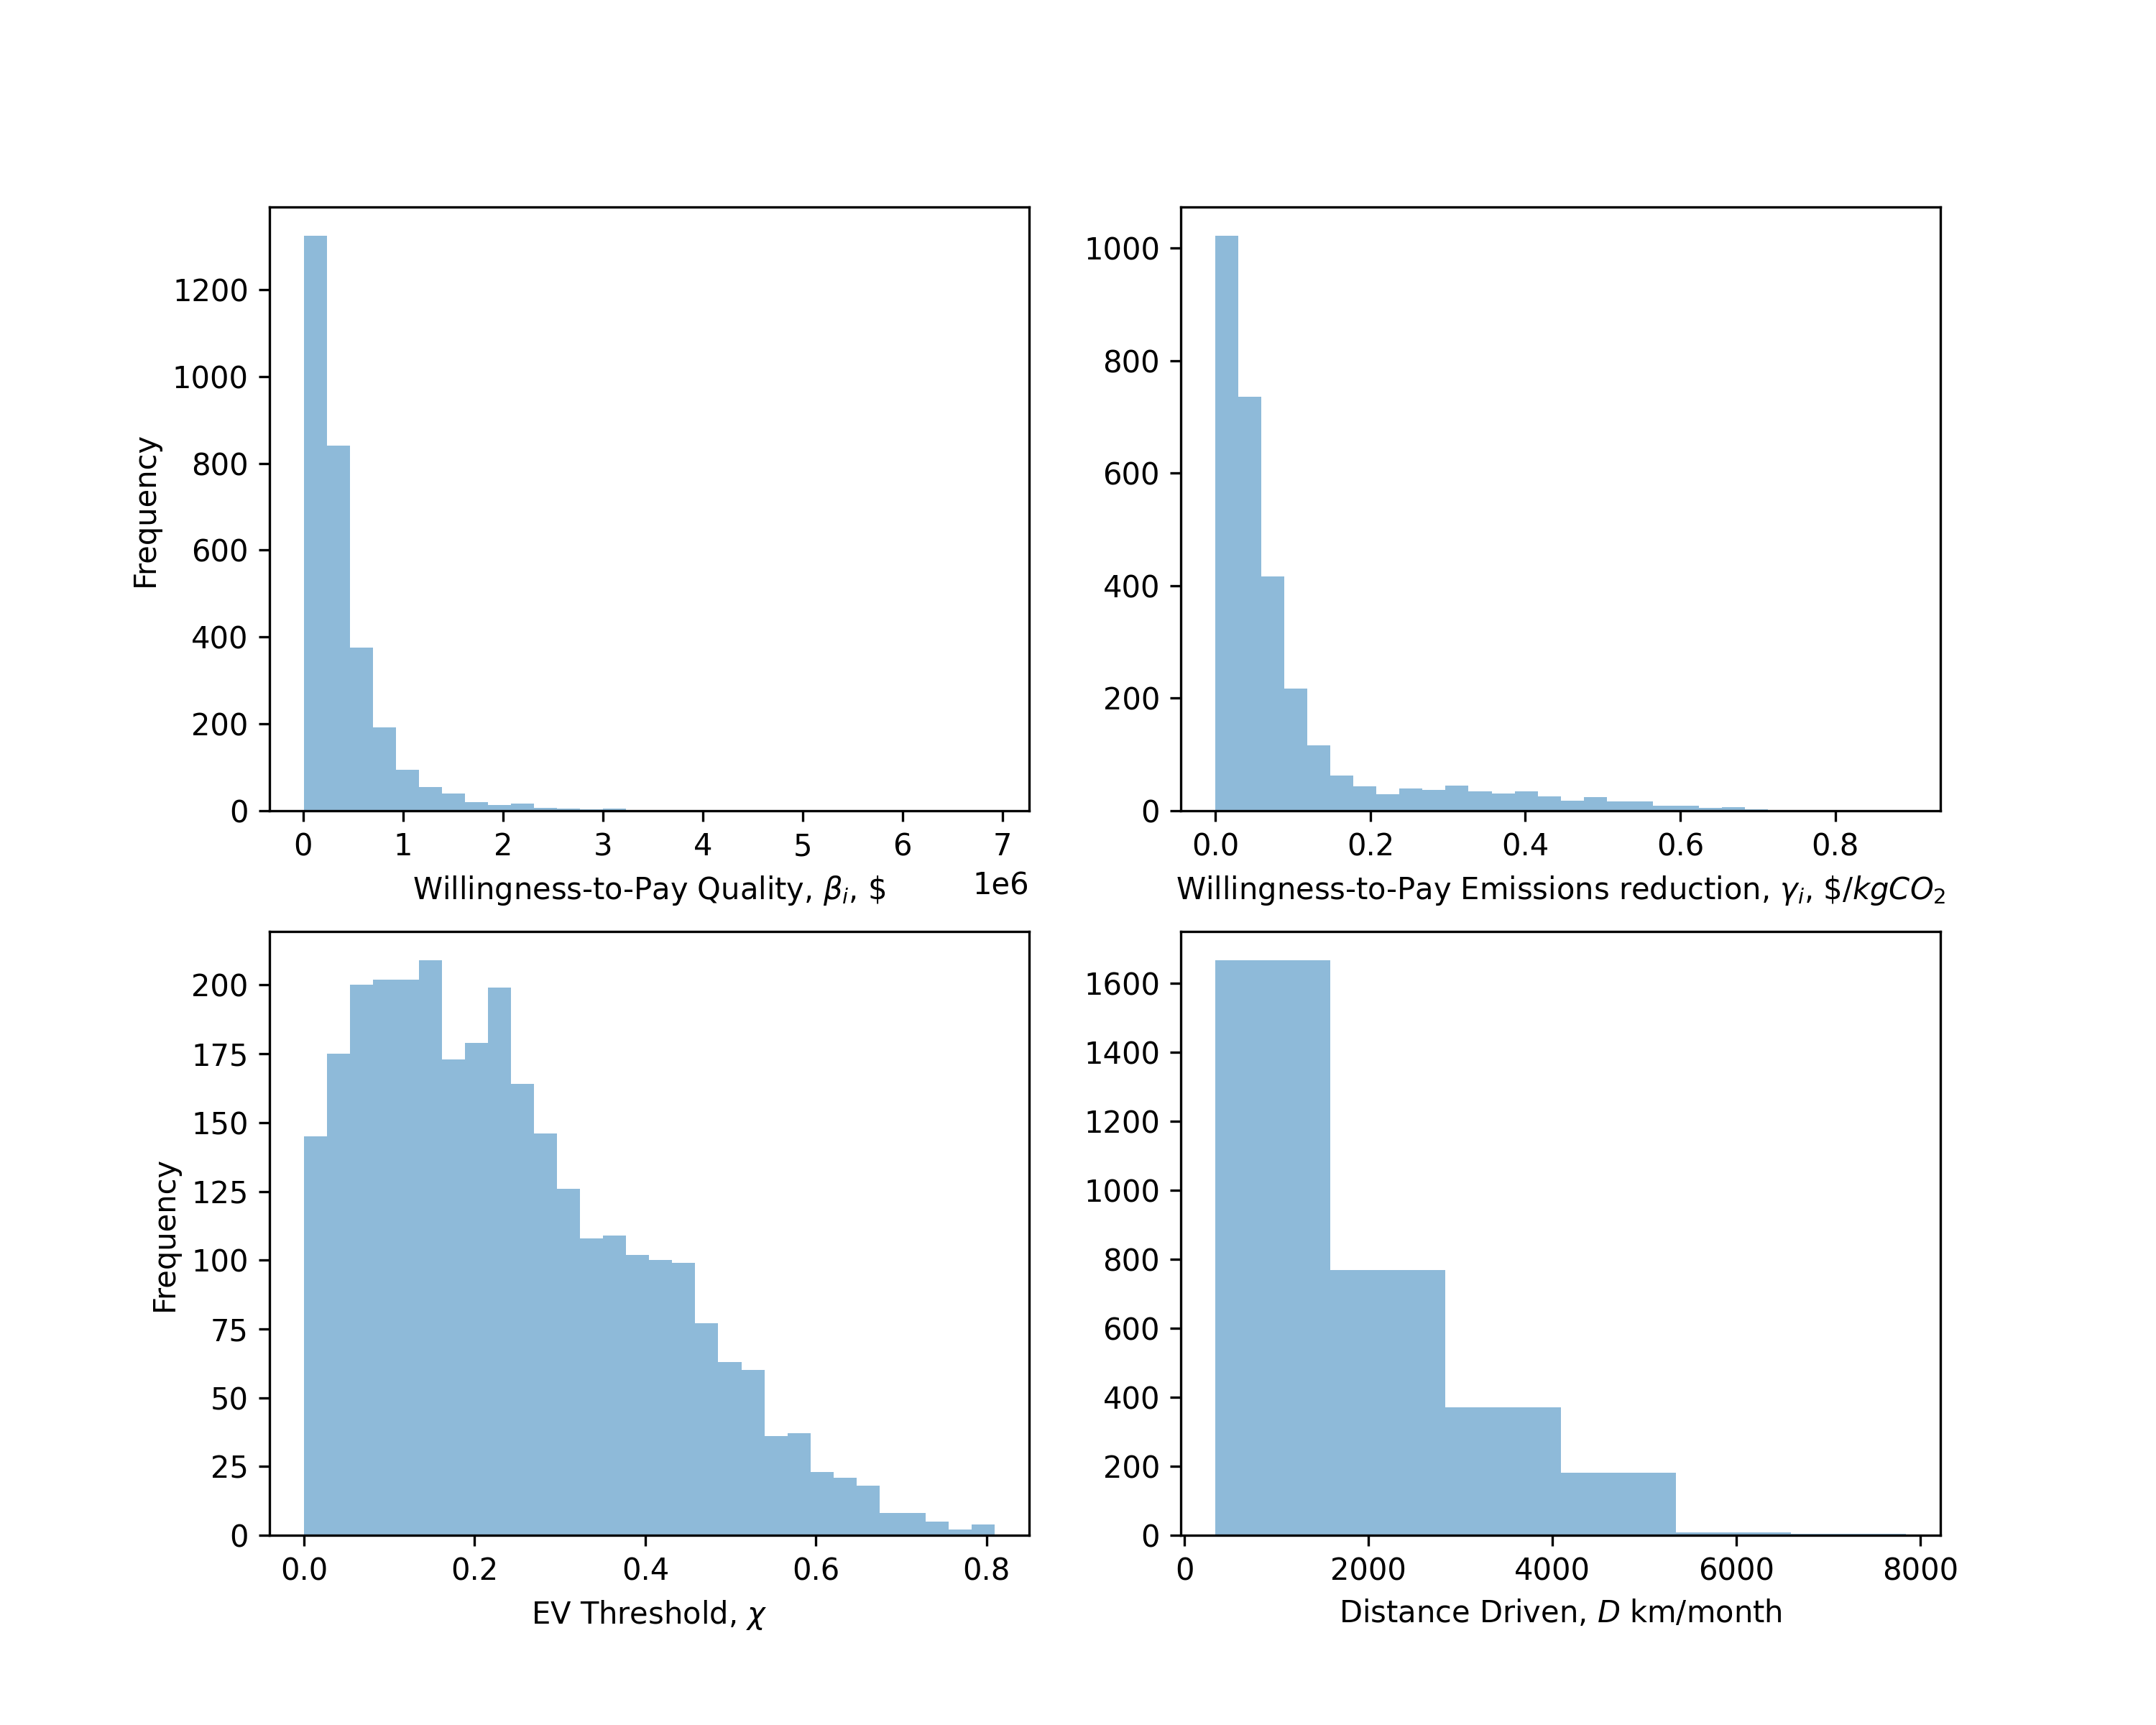
\includegraphics[width=0.9\linewidth]{Figure_6.png}
		\caption{Histogram of willingness to pay for quality (top left), willingness to pay for emissions reduction (top right), EV imitation threshold (bottom left), distance driven (bottom right).}
		\label{fig:preferences}
	\end{figure}

    \begin{figure}[H]
		\centering
		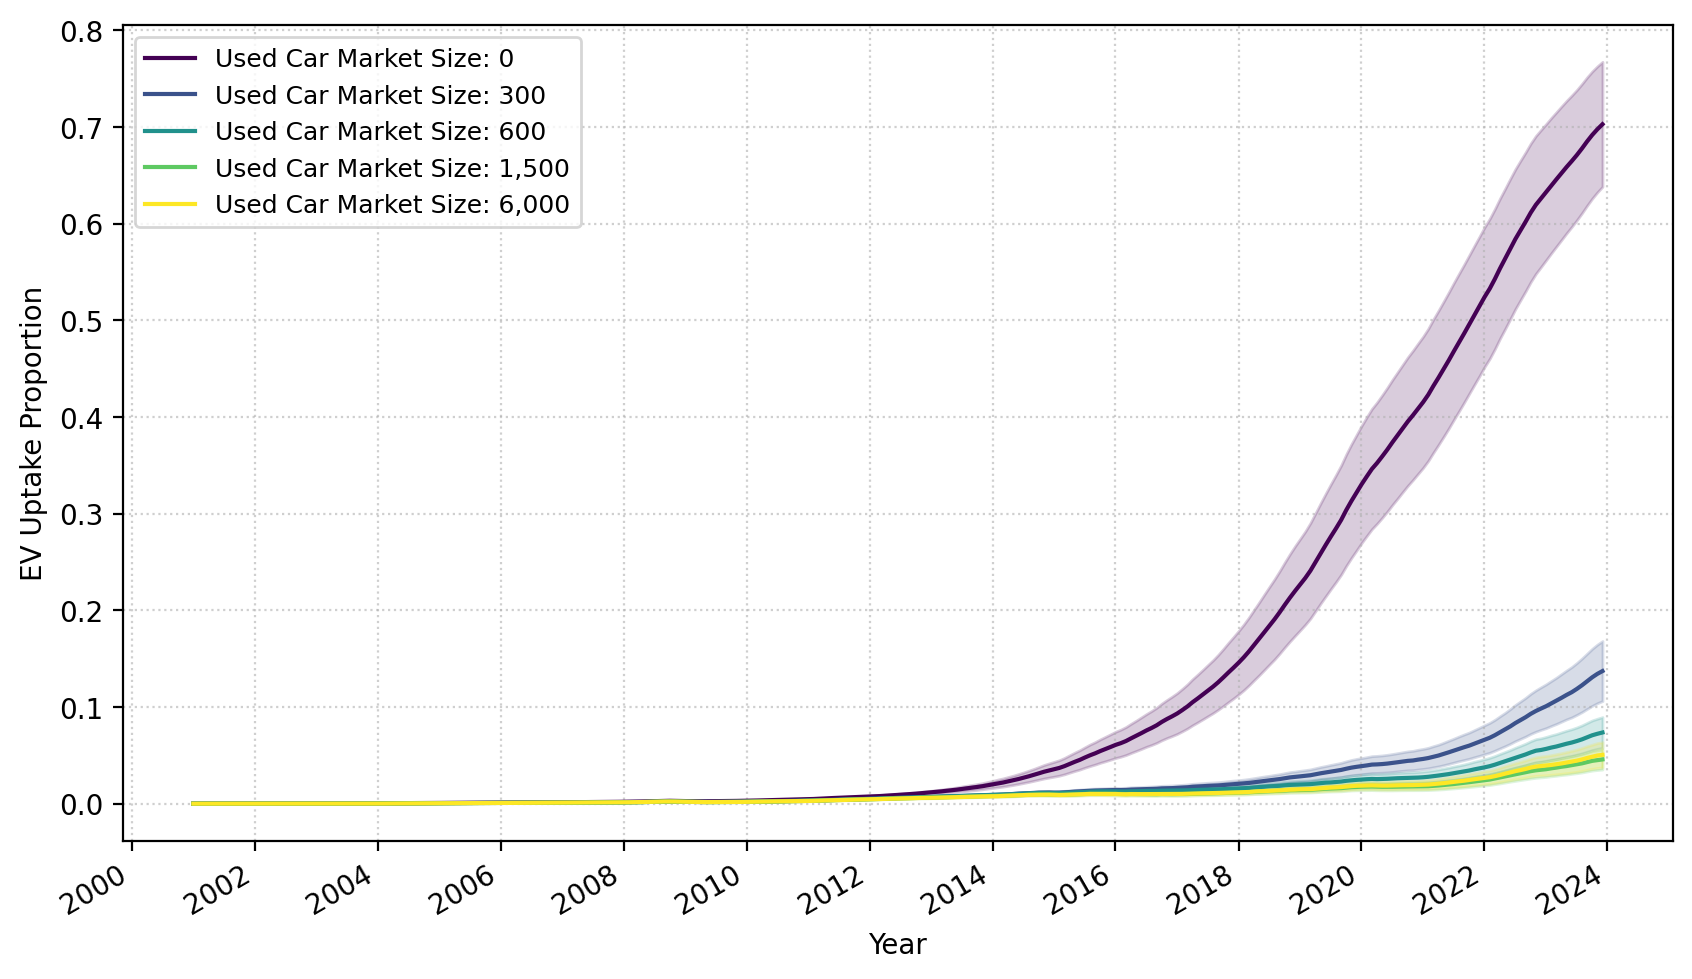
\includegraphics[width=0.9\linewidth]{Figure_7.png}
		\caption{Trend of EV uptake with varying used car market capacity with respect to population size of 3000.}
		\label{fig:used_car}
	\end{figure}
    
\end{document}